\documentclass[a4paper, oneside, 11pt]{book}
\usepackage[utf8x]{inputenc}
\usepackage[T1]{fontenc}
\usepackage{booktabs}
\usepackage{float}
\usepackage{hyperref}
\usepackage[font=small,format=hang,parskip=5pt]{caption}
\usepackage[sumlimits,]{amsmath}
\usepackage{array}
\usepackage{etex}
\usepackage{tikz, pgfplots}
\usetikzlibrary{arrows}
\tikzset {domaine/.style 2 args={domain=#1:#2} }
\usepackage{fancyhdr}
\usepackage{parskip}
\usepackage{calrsfs}
\usepackage[toc,page]{appendix}
\usepackage{titlesec}
\usepackage{algorithm,algorithmic, setspace}
\renewcommand{\algorithmicrequire}{\textbf{Input:}}
\usepackage{enumitem}
\usepackage{calc}  
\setlist[description]{leftmargin=3em,labelindent=2em}
\usepackage{acronym}
%\setlength{\parindent}{1em}
%\setlength{\parskip}{0.75em}
\setlength{\jot}{9pt}

\newcolumntype{C}{>{$}c<{$}} % math-mode version of "l" column type
\newcolumntype{L}{>{$}l<{$}} % math-mode version of "l" column type
\newcolumntype{R}{>{$}r<{$}} % math-mode version of "l" column type
\newcommand{\HRule}{\rule{\linewidth}{0.5mm}}
\definecolor{ttttff}{rgb}{0.2,0.2,1}
\definecolor{qqzzqq}{rgb}{0,0.6,0}
\definecolor{qqqqff}{rgb}{0,0,1}

\begin{document}

\frontmatter % Use roman page numbering style (i, ii, iii, iv...) for the pre-content pages
\pagestyle{plain} % Default to the plain heading style until the thesis style is called for the body content
%----------------------------------------------------------------------------------------
%    THESIS INFORMATION
%----------------------------------------------------------------------------------------




%----------------------------------------------------------------------------------------
%	TITLE PAGE
%----------------------------------------------------------------------------------------

\begin{titlepage}
\begin{center}

\vspace*{.06\textheight}
{\scshape\LARGE \href{http://www.ulb.ac.be}{Université Libre de Bruxelles}\par}\vspace{1.5cm} % University name
\textsc{\Large Master Thesis}\\[0.5cm] % Thesis type

\HRule \\[0.4cm] % Horizontal line
{\huge \bfseries  Two approaches to reduce the rank reversal occurrences in the  \textsc{promethee ii} method \par}\vspace{0.4cm} % Thesis title
\HRule \\[1.5cm] % Horizontal line
 
\begin{minipage}[t]{0.4\textwidth}
\begin{flushleft} \large
\emph{Author:}\\
{Gilles \textsc{Dejaegere}} % Author name - remove the \href bracket to remove the link
\end{flushleft}
\end{minipage}
\begin{minipage}[t]{0.4\textwidth}
\begin{flushright} \large
\emph{Supervisor:} \\
{Yves \textsc{De Smet}} % Supervisor name - remove the \href bracket to remove the link  
\end{flushright}
\end{minipage}\\[3cm]
 
\vfill

\large \textit{Mémoire présenté en vue de l’obtention du diplôme\\ 
    d'Ingénieur Civil Informaticien à finalité spécialisée \\
    \href{http://www.ulb.ac.be/facs/polytech}{Ecole Polytechnique de Bruxelles}}\\[0.3cm] % University requirement text
 
\vfill

{\large year 2016-2017}\\[4cm] % Date
%\includegraphics{Logo} % University/department logo - uncomment to place it

\end{center}
\end{titlepage}


\chapter*{\centering Acknowledgements}

I would first of all like to express my gratitude to my supervisor, Professor Yves De Smet, whose availability and advice throughout the year has been an extremely valuable help for the accomplishment of this work as well as for my personal development. 

\vskip 1cm
I would also like to thank all the members of the SMG unit for their helpfull feedback and their constructive comments.

\vskip 1cm
I address my warm thanks to my familly, particularily my father, for his multiple rereading, and my mother, which is probabily having a hard time supporting me but espacilly my brothers.


\vskip 1cm
Finally, I would like to extend my gratitude to all people who, closely or remotely, have been involved in this work, in this year, or even in my studies.

\chapter*{\centering Abstract}
\addcontentsline{toc}{chapter}{Abstract}


Some practical decision problems are complex and need to be formalised to be efficiently managed.
The decision aid discipline consists in modeling these problems.
More specifically, multi-criteria decision aid methods model them using different conflicting criteria.

Different multi-criteria decision aid methods exist but the study performed in this master thesis focus on the \textsc{promethee} methods.

Like other multi-criteria decision aid methods, \textsc{promethee ii} suffers from the rank reversal phenomenon.
This phenomenon consists in the relative ordering between two alternatives being dependant on some other alternatives of the problem.
The possibility of suffering from rank reversals can be undesirable due to manipulation threats.
Therefore, two modifications of the \textsc{promethee ii} method aimed at avoiding this phenomon have been studied.

The first modification analysed, \textsc{robust promethee}, is based on the repetition of \textsc{promethee ii} on a large number of samplings of the alternatives.
The results of this analysis show that it seems to reduce the number of rank reversals, but its efficiency in this regard strongly depends on the decision problem and on the size of the subsets on which \textsc{promethee ii} is applied.
This method introduces two new parameters: the number of iterations and the size of the samplings.
Some bounds on the minimal value of these parameters have been found.
Finally, it has been shown that some irrational results could occur (such as the non respect of the dominance relation), but with a very low probability.

A second method, \textsc{referenced promethee} has also been analysed.
It is based on the comparison using \textsc{promethee ii} of each alternative with a set of predefined reference profiles.
Since each alternative is compared with the same fixed set, this method does not suffer from the rank reversal phenomenon.
Nevertheless, it comes with the additional cost of having to find a set of fixed references.
It has been seen in this work that the rankings obtained are highly dependent on this set of reference profiles.

\newpage 
Several properties of these sets have been found. First, it is shown that a small number of references is sufficient to discriminate large set of alternatives.
Then, it is shown that it is generally even possible to replicate the rankings produced by \textsc{promethee ii} with \textsc{referenced promethee} using only this small quantity of reference profiles.
Finally, two approaches for defining these sets of reference profiles are detailed and analysed. The efficiency of each of them however strongly depends on the decision problem and it is therefore not guaranteed that they will yield set of reference profiles which lead to a satisfactory ranking.


\textit{keywords : multi-criteria decision aid, \textsc{promethee}, rank reversals, \textsc{robust promethee}, \textsc{referenced promethee}, reference profiles.}



\chapter*{\centering Résumé}
%\addcontentsline{toc}{chapter}{Resumé}

Certains problèmes d'aide à la décision sont trop complexes et doivent être formalisés pour pouvoir être appréhendés efficacement.
La discipline de l'aide à la décision consiste à modéliser ces problèmes. \\
Plus précisément, les méthodes d'aide à la décision multicritères consistent à modéliser ces problèmes en utilisant plusieurs critères de natures souvent conflictuelles.

Différentes méthodes d'aide à la décision multi-critères existent, cependant seules les méthodes \textsc{promethee} seront abordées dans ce travail.
L'une des méthodes de la famille \textsc{promethee} est \textsc{promethee ii} qui a pour but d'ordonner l'ensemble fini des solutions du problème (ces solutions sont aussi appelées des alternatives).

Comme d'autres méthodes d'aide à la décision multi-critère, \textsc{promethee ii} souffre de ce qui est appelé l'inversion de rang.
Ce phénomène consiste en ce que l'ordre relatif entre deux alternatives dépende d'autres alternatives du problème.
La possibilité pour une méthode de subir ces inversions de rang peut être indésirable. En effet, cela signifierait que celle-ci soit susceptible de subir des manipulations de rang via l'ajout ou la modification artificielle de données.
C'est pourquoi, deux méthodes dérivées de \textsc{promethee ii}, ayant pour but de réduire ces inversions de rang, sont analysées dans ce travail.

La première modification analysée, \textsc{robust promethee}, est basée sur la répétition de \textsc{promethee ii} sur une grande quantité de d'échantillons de solutions.
Les résultats de cette analyse montrent que celle-ci semble réduire le nombre de d'inversions de rangs.
Cependant, son efficacité à réduire cette quantité est fortement dépendante du problème de décision et de la taille des sous-ensembles sur lesquels \textsc{promethee ii} est appliquée.\\
Cette méthode introduit deux nouveaux paramètres: le nombre d'itérations et la taille des échantillons.
Certaines bornes sur la valeur minimale de ces paramètres ont été définies.
Enfin, il a été démontré que des résultats irrationnels peuvent être produits, mais avec une très faible probabilité.

\newpage 
Une deuxième méthode, \textsc{referenced promethee}, a ensuite été analysée.
Celle-ci est basée sur la comparaison avec \textsc{promethee ii} de chaque alternative avec un ensemble fixe de profils de référence.
Étant donné que chaque alternative est comparée au même ensemble fixe de profils, cette méthode ne souffre pas du phénomène d'inversion de rang.
Cependant, un coût additionnel consistant en la nécessité de devoir établir cet ensemble fixe de références est introduit.
Il a été observé dans ce travail que le choix de cet ensemble a un impact considérable sur le rangement final obtenu.

Plusieurs propriétés de ces ensembles de profils de référence ont été trouvées. Tout d'abord, il a été constaté qu'un large ensemble d'alternatives pouvait être départagé en utilisant un petit nombre de profils de référence.
Ensuite, il a été remarqué qu'il est en général possible de reproduire exactement le classement obtenu par \textsc{promethee ii} avec \textsc{referenced promethee} en utilisant cette petite quantité de profils de références.

Enfin, deux approches pour définir ces ensembles de profils de références sont détaillées et analysées. L'efficacité de chacune de ces deux approches dépend cependant du problème de décision, et aucune des deux ne garantit de fournir des profils de référence satisfaisants.


\textit{mots-clés: aide à la décision multicritères, \textsc{promethee}, inversion de rang, \textsc{robust promethee}, \textsc{referenced promethee}}


\tableofcontents
\chapter*{List of symbols}
\addcontentsline{toc}{chapter}{List of symbols}
%\markboth{ACRONYMS}{ACRONYMS}

This page contains a list of some symbols used in throughout this work.

{ \bf \textsc{promethee}:}
\begin{description}[leftmargin=!,labelwidth=\widthof{\bfseries $P_c()$}]
    \item[$A$] set of alternatives of the decision problem
    \item[$n$] quantity of alternatives considered
    \item[$a_i$] $i$th alternative
    \item[$k$] quantity of criteria on which the alternatives are evaluated
    \item[$f_c()$] evaluation function of the $c$th criterion
    \item[$w_c$] weight of the $c$th criterion
    \item[$\mathcal{P}$] set of the preference functions
    \item[$P_c()$] preference function of the $c$th criterion
    \item[$q, p$] indifference and strict preference thresholds of the preference functions
\end{description}

\vskip 0.4cm
{ \bf \textsc{robust promethee}:}
\begin{description}[leftmargin=!,labelwidth=\widthof{\bfseries $P_c()$}]
    \item[$R$] quantity of repetitions of \textsc{promethee ii} on the samplings
    \item[$m$] size of the samplings
\end{description}

\vskip 0.4cm
{ \bf \textsc{referenced promethee}:}
\begin{description}[leftmargin=!,labelwidth=\widthof{\bfseries $P_c()$}]
    \item[$\mathcal{R}$] set of reference profiles (also called set of references)
    \item[$p$] size of the set of reference profiles
    \item[$r$] one of the reference profiles
\end{description}


\vskip 0.4cm
{ \bf Other:}
\begin{description}[leftmargin=!,labelwidth=\widthof{\bfseries $P_c()$}]
    \item[$\tau_k$] Kendall rank correlation coefficient
\end{description}


\pagestyle{fancy}
\fancyhf{}
\lhead{\leftmark}
\rhead{ \thepage}
\renewcommand{\chaptermark}[1]{\markboth{#1}{}}

\mainmatter
\chapter{Introduction to Multi-Criteria Decision Aid}
\label{chap:mcda}

\section{Introduction to Decision aid} \label{sec:intro}

Every day, any human being has to face numerous choices (or decision problems).
Most of them are rational and therefore try to make the choices leading to the most favorable consequences.
All these decision problems appear in specific contexts that will be called the \textit{decision problem reality} or more simply, the problem reality. The contexts of decision problems can have very different natures \cite{Bertrand2002}\cite{roy1book85}: economical, political, industrial, military or even familial or personal.

The decision is not always taken by a unique person.
It can as well be taken by larger entities. These can be well defined, such as a board of directors, a council of ministers, a jury, or even a family or can be more vaguely defined such as professional pressure groups, employees of a company or the public opinion \cite{roy1book85}.

In any cases, the entity, composed by one or more people, in charge of the final decision will be called the \textit{decision maker}.

Most of the decision problems that we encounter in our daily lives are straightforward or of relatively small importance (what should we eat tonight? what movie should I watch?). They can generally be solved naturally and in a \textit{qualitative} way \cite{Bertrand2002}.
As the problem is simple and the consequences of a non optimal decision are not dramatic, it is sufficient for the decision maker to use its own experience and its assessments of the problem reality in order to choose a solution that seems optimal to him.
These kind of decision problems take most of the time place in a personal or familial context.

Some problems, on the other hand, require a more in depth reflection (should this old nuclear power plant be closed? should I invest my savings in this particular company?). \\
The decision problem reality in economical or industrial contexts have become too complex to be apprehensible in a purely qualitative manner \cite{Bertrand2002}.
Furthermore, the  choice of a good or even of the best solution for these problems can be crucial since the consequences of a bad decision can be disastrous.
In such cases, the decision maker could want to use a \textit{quantitative} approach, building a model \cite{Bertrand2002} \cite{DeSmet2013}.
In this approach, a mathematical model needs to be built. This model, which is an abstraction of the reality, will be used as support for the investigation and the communication between the different actors of the problem \cite{DeSmet2013} \cite{roy1book85}. To build this mathematical model, the consequences of each possible decision must be foreseen and quantified.

The discipline dealing with the analysis of the decision realities and the elaboration of the decision models is called operational research.
As done in \cite{Bertrand2002}, the expression \textit{decision aid} will be used as its signification is closer to the problem described.

It should also be noted that in decision aid, the quantitative and the qualitative approaches are not mutually exclusive.
The decision problem reality being generally too complex and chaotic to be entirely modelable, the quantitative approach must be combined with the qualitative one. The quantitative approach will be used to give some insight into the problem to the decision maker, which will always use his own qualitative perception  to use these insights.

In the rest of the chapter, the traditional mono-criterion approach will first be detailed. Some of it's drawbacks will then be highlighted, motivating the introduction of the multi-criteria approach that will then be detailed.

%\subsection{Steps of the decision process}
%
%The decision process can be summarized in the three following steps \cite{Bertrand2002}:
%
%\subsubsection{1. Identification of the possible decisions}
%When faced to a decision problem, the first step to do is build the space $A$ of possible decisions. From now on, the possible decisions will be called alternatives.
%
%The alternatives of a decision problem can be:
%\begin{description}
%    \item[finite and enumerable: ] the decision maker must hire one person from a set of $n$ applicants,
%    \item[finite but not enumerable:] the decision maker is facing a \textit{Travelling Salesman Problem}. As the number of possible path increases exponentially, the number of alternatives easily becomes far too great be enumerated,
%    \item[infinite:] the decision maker must choose the amount of money invested in a project.
%\end{description}
%
%\subsubsection{Preference modelling}
%All alternatives have of course not the same consequences and

\section{Mono-criterion approach}
\subsection{Formalisation and properties of mono-criterion \\ problems}

A mono-criterion decision problem can be formulated in the following way \cite{Bertrand2002}:
\begin{equation}
    Opt \{ f(a_i) \mid a_i \in A\}
    \label{eq:monocriterion_decision_problem}
\end{equation}

% The different elements of this formalisation will be detailed trough this section.
These classical models where the only one used until the end of the sixties \cite{ROY1990324}. They cover numerous families of problems and are formalised according to the three following properties. 

\subsubsection {1. $A$ forms a well-defined set of possible alternatives \cite{ROY1990324}} \label{sec:set_of_alternatives}

The set $A$ of alternatives (also called actions) forms a well-defined set. These are all the possible choices of the decision maker. This set of alternatives can be finite and enumerable, finite but not enumerable or infinite. Here under are examples of decision problem with these kinds of alternative sets:
\begin{itemize}
    \item \textbf{finite and enumerable:} the decision maker must hire one person from a set of $n$ applicants,
\item \textbf{finite but not enumerable:} the decision maker is facing a \textit{Travelling Salesman Problem}. As the number of possible path increases exponentially, the number of alternatives often becomes far too large to be enumerated,
    \item \textbf{infinite:} the decision maker must choose the amount of money invested in a project.
\end{itemize}

If the alternatives are not enumerable, the set must be defined by stating the properties (such as linear constraints) which characterise its elements \cite{Vin92}.

The set $A$ is also characterized by the following two properties \cite{Vin92}: \\
\begin{itemize}
    \item $A$ can be either \textit{stable}, if the set does not change during the decision procedure, or \textit{evolutive}, if, on the other hand, it can change. \\
There can be different reasons leading to some changes of the alternatives considered such as for example an evolving decision reality or the elimination during the intermediate steps of the procedure of alternatives that are considered not to be relevant anymore.
Consider the already mentioned example of a decision maker which has to hire one candidate from a set of applicants. It is very plausible that this set could vary during the decision process as some candidates could have found a better job elsewhere.

    \item $A$ can be either \textit{globalised}, if the decision problem consists in the selection of one unique alternative (we say that the alternatives are mutually exclusive), or \textit{fragmented} if it consists in the selection of a subset of one or more alternatives.\\
Consider for instance the problem of having to choose two locations from a set of $n$ possible locations where new warehouses would be built. This problem can be seen as fragmented if the alternatives consist in the set of $n$ locations and that two of them must be chosen, but it can also be seen as a globalised problem if the alternatives consist in the $\frac{n(n-1)}{2}$ possible couples of location and that only one must be chosen.
\end{itemize}
\subsubsection{2. The real-valued function $f(.)$ correctly reflects the preferences of the decision maker \cite{ROY1990324}}

The preferences of the decision maker are considered to be correctly represented by the unique criterion $f(.)$. This criterion must therefore synthesise on its own all the objectives of the decision maker and the consequences of each of the alternatives \cite{ROY1990324} \cite{Bertrand2002}.

Of course, this assumption can not always entirely be respected in real life decision problems. For example, a function $f(.)$ representing the profit made with the commercialisation of a product can often only be built by using estimations of the number of products that would be sold.
In such cases $f(.)$ could be subject to some subjectivity.
This specific kind of subjectivity should be avoided as much as possible as it introduces some imprecisions. The reality should be represented as accurately possible by the evaluation function $f(.)$. 
Some other kind of subjectivity, which is essential and should therefore not be avoided, will be introduced in the section concerning the multi-criteria approach.

The problem could consist in minimising this criterion (e.g. $f(.)$ represents a cost) or to maximise the criterion (e.g. $f(.)$ represents a profit). Without loss of generality, for the rest of this section we will consider that $f(.)$ is a criterion to maximise.

\begin{equation}
    Max \{ f(a_i) \mid a_i \in A \}
    \label{eq:monocriterion_maximise}
\end{equation}

\subsubsection{ 3. The decision problem forms a well-formulated mathematical problem \cite{ROY1990324}}

If a mono-criterion decision problem is modeled as \eqref{eq:monocriterion_maximise} with $A$ being a finite set, then there exists at least one solution such that:

\begin{equation}
    f(a_i^*) \ge f(a_j), \forall a_j \in A
    \label{eq:monocriterion_optimal_solution}
\end{equation}

Such solutions are said to be optimal for the decision problem. These are entirely determined by the modelling of the problem. The process of finding such an optimal solution is a classical optimisation problem, leading to the discovery of some ``hidden truth'' \cite{ROY1990324}\cite{Vin92}. Indeed, if the decision maker approves the model, he should adopt one of the proposed optimal solutions.

\subsubsection{4. Additional properties of the mono-criterion problem}
With a mono-criterion problem, more can be done than finding an optimal solution. Indeed, $f(.)$ implies a natural dominance relation ($P$,$I$) on every pair of elements of $A$ \cite{Bertrand2002}:

\begin{equation}
    \forall a_i, a_j \in A: \left\{
        \begin{array}[]{l c c c c}
            f(a_i) & > & f(a_j) &\Leftrightarrow & a_iPa_j \\
            f(a_i) & = & f(a_j) &\Leftrightarrow & a_iIa_j \\
            f(a_i) & < & f(a_j) &\Leftrightarrow & a_jPa_i \\
        \end{array}
        \right .
    \label{eq:dominance_relation_monocriterion}
\end{equation}
where $P$ and $I$ respectively stand for preference and indifference.

The preference structure of this relation forms a \textit{complete preorder} \cite{Vin92}. All the alternatives can be ranked from the best one to the worst one (complete) with eventual ties between two alternatives (preorder).

By nature, the following properties of $P$ and $I$ should also be noted \cite{Vin92}:
\begin{equation}
    \forall a_i,a_j \in A \left \{
        \begin{split}
            a_iPa_j \Rightarrow a_j \neg P a_i &: \text{ P is asymmetric} \\
            a_iIa_i &: \text{ I is reflexive} \\
            a_iIa_j \Rightarrow a_j I a_i &: \text{ I is symmetric} \\
        \end{split}
        \right .
    \label{eq:properties_P_I}
\end{equation}

\subsection{Drawback of the mono-criterion approach} \label{sec:drawback_monocriteria}
Two main drawbacks of the mono-criterion approach are underlined in \cite{Bertrand2002}.
The first one is that, if the decision maker wants to take a decision according to several points of view (e.g. cost, sustainability, equity, \dots), a single criterion can generally not synthesise the decision problem reality.
This is illustrated with the following example taken from \cite{roy1book85}.\\
Suppose you are working in a rubber manufacturing firm and that you need to design a new rubber to respond to the needs of a customer.
Your task will be to choose, between the different possible compositions of the rubber, one that best fulfills the specified requirements.
Depending on these possible requirements you will probably have to choose a composition with a high breaking strength, a limited thermal conductivity, a certain elasticity, and that all these characteristics are valid for a range of temperature as large as possible. The client will probably also require that these properties do not deteriorate too quickly with time. He could also require that the rubber does not react with a specific paint with which it will be painted. Finally, you will also have to find a composition that minimises the cost of production.\\
It can be concluded from this example that it is not always realistic to hope to find a unique criterion synthesising correctly all the aspects of the decision problem reality.

The second drawback of the mono-criterion approach is that the classic notion of a criterion is only used in order to compare if the evaluation of an alternative $a_i$ is greater, smaller, or equal to the evaluation of an alternative $a_j$. This information could be misleading.\\
If we consider again the problem of choosing a composition for the new rubber but this time only focusing on the expected lifetime criterion. A composition which is expected to maintain his required properties for 45 years will be preferred over a composition maintaining its properties for 40 years in the same way that it would be preferred over a third composition maintaining its properties for 5 years.\\
This often does not represent the reality accurately. Suppose that the rubber is aimed to be used to manufacture parts of a car.
Both 40 year and 45 year would therefore be considered as perfectly fine expected lifetimes and the difference between those two compositions would generally be considered as neglectable.
The two compositions would then be equally preferred.
On the other hand, an expected lifetime of 5 years is insufficient.
In the classical mono-criterion approach, however, the rubber compositions whose expected lifetime is 45 years will be preferred over the one of 40 years exactly in the same that it will be preferred over the one whose expected lifetime is 5 years. This is misleading.

For these reasons, the mono-criterion approach is not always adapted and some decision problems require a multi-criteria one. As it can easily be guessed, this second approach tackles the drawbacks mentioned above by introducing several evaluation criteria. This approach will be detailed in the next section.

\section{Multi-Criteria Approach} \label{sec:Multi-criterion_approach}

A multi-criteria decision problem can be modeled in the following way \cite{Bertrand2002}:
\begin{equation}
    Opt \  \{f_1(a_i), f_2(a_i), \cdots , f_c(a_i), \cdots , f_k(a_i) | a_i \in A\}
    \label{eq:multicriteria_pb_model}
\end{equation}
With $A$, the set of alternatives, and $f_c(.), c=1,\cdots ,k$, a set of $k$ evaluation criteria which are applications of $A$ on the set of real numbers. \\

The definition of the set of alternatives does not change from the mono-criterion case (section \ref{sec:set_of_alternatives}).\\
The set of alternatives can be defined by an enumeration of each of the alternatives if these are enumerables. If the set is too large, it must be defined by the properties characterizing its alternatives.
The set of alternatives can be stable or evolutive and globalized or fragmented.

In the rest of this work, all multi-criteria decision aid methods that will be considered must be applied on a finite set of alternatives with a finite family of criteria. Without loss of generality, we will therefore only consider decision problems consisting in a set $A$ of $n$ alternatives evaluated on $k$ criteria that must be maximised.
\begin{equation}
    \max \  \{f_1(a_i), f_2(a_i), \cdots , f_c(a_i), \cdots , f_k(a_i) | a_i \in A\}
    \label{eq:multicriteria_pb_model_maximisation}
\end{equation}

\subsection{Mathematically ill-defined problem}

In opposition to the mono-criterion decision problem, the concept of optimal solution does not make sense anymore in a multi-criterion context.
Indeed, due to the usually conflicting nature of the different criteria considered in a decision problem reality, it is generally not possible to find an alternative $a_i$ such that:

\begin{equation}
    f_c(a_i) \ge f_c(a_j), \forall a_j \in A, \forall c = 1, \dots,k
    \label{eq:no_optimal_sol_mutlicriterion}
\end{equation}

The problem in this case does not consist anymore in the discovering of some hidden truth. It will consist in finding one or more alternatives that consist in a good compromise on all the criteria.
The quality of a compromise is of course strongly dependent on the decision maker's perception of the problem reality. Some subjectivity must therefore explicitly be introduced. This subjectivity can be associated with the qualitative approach presented in section \ref{sec:intro}.

It has already been seen in the mono-criterion approach that some subjectivity could be involuntarily introduced when building the evaluation function $f(.)$.
This kind of subjectivity however should still be avoided in the multi-criteria approach.

\subsection{Types of multi-criteria decision problems} \label{sec:type_of_pb}
As shown by B. Roy, there exist different types of decisions problems \cite{Bertrand2002}. Here under are three examples of common types:
\begin{itemize}
    \item \textit{ Choice Problems}: these consist in choosing one or several alternatives from $A$ which could be considered as the best alternatives. One example of a choice problem could be the already mentioned problem of choosing the two most adapted locations to build new warehouses.
    \item \textit{ Ranking Problems}: these consist in the partially ordering all the alternatives from the worst to the best one. One example of an ordering problem could be the following one: $n$ nuclear power station must be closed. However, it is not possible to close all these stations simultaneously. In which order should they be closed to minimise the risk and the cost.
    \item \textit{ Sorting Problems}: these consist in sorting (or partially sorting) all the alternatives in different categories. One example of sorting problem is given hereafter.
Consider $n$ patients that are sent to a liver specialist to assess whether or not these patients need a liver transplant. The specialist could have to classify these patients in three categories, the ones who do not need a transplant, the one who need a transplant, and the ones who need a transplant with urge.
\end{itemize}

More examples of decision problem types with some applications of these problems can be found in \cite{DeSmet2013}.

\subsection{Dominance relation} \label{sec:multi_criteria_dominance_rel}

The natural dominance relation defined in a mono-criterion context (equation \ref{eq:dominance_relation_monocriterion}) is generalized to a multi-criterion context as follow \cite{Bertrand2002}:

\begin{equation}
  \label{eqn:IP}
  \forall a_i, a_j \in A: \left\{
    \renewcommand{\arraystretch}{1.75}
    \begin{array}{l l}
      a_iPa_j  & \Leftrightarrow \quad \left\{
          \begin{array}{l l}
              f_c(a_i)\ge f_c(a_j) \quad \forall c=1\dots k \\
              \exists h: f_h(a_i) > f_h(a_j) \\
          \end{array} \right . \\
      a_iIa_j & \Leftrightarrow \quad f_c(a_i) = f_c(a_j) \quad \forall c=1 \dots k \\
      a_iRa_j & \Leftrightarrow \quad \left\{
          \begin{array}{l l}
              \exists h: f_h(a_i) > f_h(a_j) \\
              \exists h': f_{h'}(a_i)< f_{h'}(a_j) \\
          \end{array} \right . \\
    \end{array} \right .
\end{equation}
where $P$ and $I$ still stand for preference and indifference and $R$ stands for incomparability.
The preference structure of this relation is a \textit{partial preorder} structure \cite{Vin92} as only some subsets of alternatives can be ranked from ``best'' to ``worst'' with eventual ties.

As the preference and indifference relation require unanimity on all the criteria, and the incomparability relation only needs two conflicting criteria, one can easily convince himself that the dominance relation is generally very poor, and that most pairs of alternatives will be incomparable.\\
The main objective of the multi-criteria decision aid methods will be to enrich this dominance relation by reducing the number of incomparable pairs of alternatives. The final ordering of the alternatives is, as it will be seen here under, not only dependent on the decision maker, but also on the decision method used to enrich the dominance relation.

\subsection{Types of multi-criteria decision aid methods}

Multi-criteria decision aid methods can be divided in three families of methods \cite{Bertrand2002}:
\begin{enumerate}
    \item Aggregating methods (Multi-attribute utility theory)
    \item Outranking methods
    \item Interactive methods
\end{enumerate}

\subsubsection{Aggregation methods (Multi-attribute utility theory)}
Aggregating methods consist in the substitution of a multi-criterion decision problem into a mono-criterion one.
This is done by synthesising all of the $k$ criteria of the multi-criteria problem, into a unique utility function $U(a_i)$:
\begin{equation}
    U(a_i) = U[f_1(a_i), \dots, f_k(a_i)]
    \label{eq:utility_fct}
\end{equation}

The problem is therefore summarised to:
\begin{equation}
    Max \{U(a_i) \mid a_i \in A \}
    \label{eq:maut_model}
\end{equation}

A usual way to select an utility function is to build it as a sum of all the criteria evaluations \cite{Vin92}:

\begin{equation}
    U(a_i) = \sum\limits^k_{c=1} U_c(f_c(a_i))
    \label{eq:maut_additive_utility_function}
\end{equation}

This kind of utility function will constitute the additive model. 
The role of the different $U_c(.)$ functions must be at least to normalise all the criteria to get rid of all scaling effects introduced by the measuring scale in which the criteria are expressed.
This is not the only role of these functions. They could for example also be used to manage criteria evaluations that should neither be maximised nor minimised but which should be as close as possible to a desired value. $U_c(.)$ could then be maximal when $f_c(a_i)$ is equal to that desired value.

Another formulation can also be used to compute the utility function of the alternatives:
% In a second time, some weight factors $w_c$ can also be introduced to express the relative importance of each criterion according to the decision maker:


\begin{equation}
    U(a_i) = \sum\limits^k_{c=1} w_c \cdot U_c(f_c(a_i))
    \label{eq:maut_additive_utility_function_weighted}
\end{equation}
Here, some weight factors $w_c$ are introduced to express the relative importance of each criterion according to the decision maker.
In equation \ref{eq:maut_additive_utility_function}, the effect of these coefficients were obtained by selecting an adequate $U_c(.)$ function but the two are kept distinct in equation \ref{eq:maut_additive_utility_function_weighted} to emphasise their respective meaning.

It is quite obvious that the preference structure of such a problem will be the same as in a mono-criterion context. The dominance relation will therefore form a complete preorder.

This seems at first sight to solve all the problem introduced by the different criteria. Unfortunately, these methods have some drawbacks. First of all, in such additive models, a very bad evaluation on one criterion can be completely compensated by better performances on the other criteria.

Let's consider once again, the example of having to choose a rubber composition. Let's suppose we are evaluating the two only possible alternatives, $\mathcal{R}_1$ and $\mathcal{R}_2$, according to four following criteria: \textit{breaking strength, price, thermal conductivity and expected lifetime}. \\
To get rid of any scaling effect, the $U_c(.)$ functions will assign to each criterion a score between $0$ and $100$ according to the preferences of the decision maker.

Suppose, once again, that the rubber is aimed at manufacturing car parts and that one of the two alternatives ($\mathcal{R}_1$) has an expected lifetime of 5 years. The decision maker will therefore give its ``expected lifetime'' evaluation a value of 0.

The evaluation table of the two alternatives could be similar to the following one:
\begin{table}[h]
\center
\begin{tabular}{ l c c c c c}
    \toprule
     &  &  \multicolumn{4}{c}{$U_c(.)$} \\
     \cmidrule{3-6}
     Alternatives & & Breaking strength & Price & Conductivity & Lifetime  \\
     \cmidrule(rl){1-1}   \cmidrule{3-6}
      $\mathcal{R}_1$  & & 100      & 40    & 90      & 0   \\
      $\mathcal{R}_2$  & &50       & 50    & 50      & 50  \\
    \cmidrule(lr){1-6}
    Weights   & &0.5      & 0.2   & 0.15    & 0.15 \\
    \bottomrule
\end{tabular}
\caption{evaluation table for the rubber composition problem using an MAUT method}
\label{tbl:maut_compensation_bad_criterion}
\end{table}

From this table it can easily be seen that even if the evaluation on the ``expected lifetime'' criterion of the first alternative is the worst possible, the total utility function $U(\mathcal{R}_1)$ will be equal to $0.5\cdot 100+ 0.2 \cdot 40 + 0.15\cdot 90 = 71.5$. This is greater than the utility function $U(\mathcal{R}_2)$ which is equal to $0.5$.

Using this additive model, a good rubber composition, but with an unacceptable expected lifetime, could be preferred over a compromise composition. 
%There is therefore no notion of veto.

Another possible problem of the additive model is that not all preferences of a decision maker can be represented.

Let's for example consider the following example proposed by Vincke \cite{Vin92}:

\begin{table}[h]
\center
\begin{tabular}{@{} L  L L L L L L L L L @{}}
    \toprule
      a_i: & a_1 & a_2 & a_3 & a_4 & a_5 & a_6 & a_7 & a_8 & a_9 \\
    \midrule
     f_1(a_i) &1  &1 &1 &2 &2 &2 &3 &3 & 3\\
     f_2(a_i) &1  &3 &5 &1 &3 &5 &1 &3 &5 \\
    \bottomrule
\end{tabular}
\caption{evaluation for a potential decision maker}
\label{tab:evaluation_example_vinck}
\end{table}

Suppose that the preferences of the decision maker are the following ones:
\begin{equation}
    a_9Pa_6Pa_8Pa_5Pa_3Ia_7Pa_2Ia_4Pa_1
    \label{eq:example_vinck_pref_structure}
\end{equation}

This global preference can not be represented using an additive function. \\
Indeed by the definition of the indifference relation in a mono-criterion context (section \ref{eq:dominance_relation_monocriterion}), and therefore valid for a aggregating method:
\begin{equation}
    \begin{split}
        a_2Ia_4 & \Rightarrow U(a_2) = U(a_4) \\
        & \Rightarrow  \sum\limits^k_{c=1} w_c \cdot U_c(f_c(a_2)) = \sum\limits^k_{c=1} w_c \cdot U_c(f_c(a_4)) \\
        & \Rightarrow w_1 U_1(1) + w_2 U_2(3) = w_1 U_1(2) + w_2  U_2(1) \\
        & \\
        a_3Ia_7 & \Rightarrow U(a_3) = U(a_7) \\
        & \Rightarrow  \sum\limits^k_{c=1} w_c \cdot U_c(f_c(a_3)) = \sum\limits^k_{c=1} w_c \cdot U_c(f_c(a_7)) \\
        & \Rightarrow w_1 U_1(1) + w_2 U_2(5) = w_1 U_1(3) + w_2  U_2(1) \\
    \end{split}
\end{equation}
If we subtract the second equation to the first one, we obtain the following equality:
\begin{equation}
    \begin{split}
    w_1 U_1(3) + w_2 U_2(3) = w_1 U_1(2) + w_2 U_2(5) \\
    \sum\limits^k_{c=1} w_c \cdot U_c(f_c(a_8)) = \sum\limits^k_{c=1} w_c \cdot U_c(f_c(a_6)) \\
    \end{split}
    \label{eq:example_vincke_step2}
\end{equation}
which is in contradiction with $a_6Pa_8$.

Of course, not being able to model all possible preferences of a decision maker is not a problem since all possible preferences are not necessarily rational.
A decision maker could for example prefer an alternative that is strictly worse than another for any concerned criterion.
Useful decision aid methods could not be able to produce such outputs as they are expected to produce rankings which should be considered as rational for the given decision problem modelisation.\\
%Useful decision aid method could not be able to produce such outputs as they are expected to produce rational rankings. \\
However, this is not the case in this example where it is not possible to reproduce the preferences of a decision maker which seem rational and coherent with the problem modelisation.
This is, in fact, not a particularity of aggregating methods. There are often preferences which are not compatible with how the multi-criteria decision aid method models the problem reality.

There exist other models than the additive model, but, as already stated, the additive model is the most commonly used in practice \cite{Vin92}.

The result of the application of a multiple attribute theory method leads to a complete preorder of all the alternatives. This preorder generally contains far more information than the natural dominance relation defined on the initial multi-criteria problem.
This abundant quantity of information is due to the theory's strong assumptions (e.g. existence of a function $U$, additivity) and to the vast amount of information asked to the decision maker (e.g. preference intensities, \dots) \cite{Vin92}.

Building a complete preorder may seems too radical as the data available with the problem is not always sufficient to compare all alternatives.
Furthermore, keeping some alternatives incomparable can give some insights to the decision maker about the conflicting nature of the criteria in a specific multi-criteria problem.

To deal with this problem, B. Roy introduced the concept of \textit{outranking relations} and \textit{outranking methods}. These concepts will be detailed here under.



\subsubsection{Outranking methods}

Outranking relations are relations aimed at enriching the dominance relation which is considered too poor, but in a realistic way.
This is, not as much as with an utility function which is considered too rich to be reliable \cite{Bertrand2002}.

B. Roy defines the outranking relation as \cite{roy1book85}:

\begin{quote}
\textit{    
``a binary relation $S$ defined in $A$ such that $aSb$ if, given what is known about the decision-maker's preferences and given the quality of the valuations of the actions and the nature of the problem, there are enough arguments to decide that $a$ is at least as good as $b$, while there is no essential reason to refute that statement.''}
\end{quote}

The outranking relations have a different mathematical formalization in each outranking method.
For instance, Roy's definition given here above describes a binary relation, meaning that the alternative $a_i$ either outranks another alternative $a_j$ either does not outranks this alternative, but an outranking relation could also be valued and give an indication of how $a_i$ outranks $a_j$. 

These relations must not be complete (as already suggested) and must neither be transitive. 

The \textsc{promethee} methods are outranking methods using an valued relation and will be explained in details in the following chapter.

Here under is a brief description of the \textsc{electre i} method.

\subsubsection{\textsc{electre i} } \label{sec:electre}


\textsc{electre} is a family of multi-criteria decision aid methods whose name stand for ``ELimination Et Choix Traduisant la REalité'' (elimination and choice expressing reality).

%The \textsc{electre i} multi-criteria decision aid method must be applied on a finite set $A$ of alternatives, with a finite set of $k$ evaluations functions (that will as usual suppose to be functions that must be maximised).

\textsc{electre i} is a multi-criteria decision aid method of the \textsc{electre} family. It is based on the construction of an binary outranking relation $a_iSa_j$, meaning that $a_i$ is at least as good as $a_j$. This relation is built according to two indices \cite{Roy1968}: the \textit{concordance} index and the \textit{discordance} index.
These indices are computed as follows.

Given two alternatives $a_i$ and $a_j$, the set of criteria $C(a_i,a_j)$ is the subset of all the criteria composed of the criteria $c$ where the evaluation of $a_i$ is better or equal than the evaluation of $a_j$.

If we suppose once again that the multi-criteria decision problem is composed of $k$ criteria to maximise, we can define $C(a_i,a_j)$ as:
\begin{equation}
    C(a_i,a_j) = \{c=1\dots k \mid f_c(a_i) \ge f_c(a_j)\}
    \label{eq:electre_concordance_set}
\end{equation}

This set of criteria includes all the criteria in concordance with $a_iSa_j$ \cite{Roy1968}. The other criteria, that are not included in $C(a_i,a_j)$, form another subset $D(a_i,a_j)$. This subset includes all the criteria that are in discordance with $a_iSa_j$.

To be able to use these two sets consistently, some relative importance factor must be assigned to each criterion in order to be able to measure the importance of the two sets. \\
With these factors $w_c$, we can compute a concordance index $c(a_i,a_j)$ \cite{Roy1968}:
\begin{equation}
    c(a_i,a_j) = \frac{1}{W}\sum\limits_{\substack{c \in \\ C(a_i,a_j)}} w_c \quad \text{ with } W=\sum\limits_{c=1}^k w_c
    \label{eq:electre_concordance_index}
\end{equation}

There are different ways of computing the discordance index $d(a_i,a_j)$, such as the one described in \cite{Roy1968}:
\begin{equation}
    d(a_i,a_j) = \left \{
        \renewcommand{\arraystretch}{1.75}
        \begin{array}{ l l l }
            0 & \text{if } D(a_i,a_j) = \emptyset  \\
            \dfrac{1}{d}  \max\limits_{\substack{c \in \\ D(a_i,a_j)}}[f_c(a_j)-f_c(a_i)] & \text{if } D(a_i,a_j) \neq \emptyset  \\
        \end{array}
        \right . \\
    \label{eq:electre_discordance_index}
\end{equation}
with
\begin{equation}
    d = \max\limits_{c, i, j} \mid f_c(a_i) - f_c(a_j) \mid
    \label{eq:electre_max_ecart}
\end{equation}
being the maximal difference of two alternatives on any criterion.

The concordance index and the discordance index both have values in the range $[0,1]$. The concordance index $c(a_i,a_j)$ increases as the number of criteria for which $a_i$ is preferred or indifferent over $a_j$ increases. It represents the relative importance of the coalition of criteria for which $a_i$ is preferred. \\
The discordance index increases as the maximal gap between an evaluation of $a_j$ and an evaluation of $a_i$ (where $a_j$ is preferred) increases. This index can be seen as the veto power to reject that $a_i$ outranks $a_j$.


Using these two indices, the outranking relation $S$ will be built as follow:

\begin{equation}
    \forall a_i, a_j \in A, a_iSa_j \Leftrightarrow \left \{
        \begin{array}[]{l}
            c(a_i,a_j) \ge p \\
            d(a_i,a_j) \le q \\
        \end{array}
        \right .
    \label{eq:electre_dominance_relation}
\end{equation}

with $p$ and $q$ being the concordance and discordance thresholds defined by the decision maker.

Once the outranking relation is built, it must still be exploited. We can represent the problem as a graph having as vertices the alternatives of the problem. The graph will have a directed edge from the vertice $a_i$ to the vertice $a_j$ if and only if $a_iSa_j$. We will therefore denote it as the outranking graph of the decision problem.

The \textsc{electre i} method was designed for the multi-criteria choice problems (see section \ref{sec:type_of_pb}).
It is aimed at finding a subset $N$ of alternatives such that no alternative in $N$ is outranked by any other alternative in $N$ and all alternatives in $A\setminus N$ are outranked by at least one alternative of $N$.

\begin{equation}
    \left \{
        \begin{array}[]{l}
            \forall a_j \in A \setminus N, \ \exists a_i \in N: a_iSa_j \\
            \forall a_i, a_j \in N: a_i \neg S a_j \\
        \end{array}
        \right .
    \label{eq:electre_graph_kernel}
\end{equation}
The problem of finding a subset $N$ of alternatives fulfilling these conditions is the problem of finding a kernel of the outranking graph.


\section{Conclusion}

As it has been seen, some decision problem can be more efficiently handled using a multi-criteria approach. There exist different type of multi-criteria decision aid methods, each having their advantages and their drawbacks.
% The next chapter will introduce the \textsc{promethee} methods and the \textsc{promethee ii} method. The main focus of the rest of this work will be the study of two variations of the \textsc{promethee ii} method.

The next chapter will introduce the \textsc{promethee} family of methods and the main focus of the rest of this work will be the study of two variations of \textsc{promethee ii}.


\chapter{Introduction to the \textsc{promethee} methods}
\label{chapterPromethee}

The \textsc{promethee} (Preference Ranking Organisation METHod for Enrichment Evaluations) methods are outranking methods that have been developed at the \textsc{Universit\'{e} Libre de Bruxelles} and the \textsc{Vrije Universiteit Brussel} since the beginning of the 80'.
Initially proposed by J.P. Brans in 1982,  %maybe make citation
they are used to address multi-criteria problems.

The \textsc{promethee} family is relatively young compared to some other multi-criteria decision aid methods but have experienced a rapid spread as it can be seen from the increasing amount of papers that are written each year about them \cite{Behzadian2010198}.

The \textsc{promethee} methods must be applied on problems with a finite set of alternatives and a finite family of criteria.
The information about each alternative and its evaluations for each criterion can be summarized in a table such as Table \ref{tbl:evaluation_table}.

\begin{table}[h]
\center
\begin{tabular}{ L @{\hskip 1cm}L L L L L}
    \toprule
    a        & f_1(.)               & \dots  & f_c(.)        & \dots  & f_k(.) \\ [7pt]
    \midrule
    a_1      & f_1(a_1)             & \dots  & f_c(a_1)      & \dots  & f_k(a_1)\\
    \vdots   & \vdots               & \ddots & \vdots        & \ddots & \vdots \\
    a_i      & f_1(a_i)         & \dots  & f_c(a_i)  & \dots  & f_k(a_i)  \\
    \vdots   & \vdots               & \ddots & \vdots        & \ddots & \vdots \\
    a_n      & f_1(a_n)             & \dots  & f_c(a_n)      & \dots  & f_k(a_n)\\
    \bottomrule
\end{tabular}
\caption{example of evaluation table}
\label{tbl:evaluation_table}
\end{table}

\newpage

This raw information is generally not directly usable by the decision maker.
 \textsc{promethee} offer some tools to help him in his ordering, choice, sorting problem, etc.

These methods are based on the three followings concepts \cite{Bertrand2002}:
\begin{enumerate}
    \item \textbf{Enrichment of the preference structure } \\
        For each criterion, a preference function is introduced.
        These preference functions are aimed at indicating the degree at which one alternative is prefered over another for that specific criterion.
        This is done by taking into account the deviation's amplitude between the evaluations of the two alternatives regarding the concerned criterion.
        This leads to an enriched intra-criterion preference structure of the alternatives. \\
        This procedure also allows to get rid of all the scaling effects due to the measuring system used to express the different criteria.
    \item \textbf{Enrichment of the dominance relationship} \\
        For each couple of alternatives, a global preference index of the one over the other will be computed using the previously defined preference functions on all the criteria.
        Using these global preference indices, a quantitative outranking score is computed.
    \item \textbf{Decision support} \\
        An outranking relation is used to rank the alternatives according to their outranking scores. This relation is used to provide some insights to the decision maker.
\end{enumerate}

\section{Enrichment of the preference structure}
\label{sec:pref_struct}

First of all, let us introduce the notation $d_c(a_i,a_j)$ that will represent the difference between $f_c(a_i)$ and $f_c(a_j)$:
\begin{equation}
    d_c(a_i,a_j) = f_c(a_i) - f_c(a_j)
    \label{eq:dc}
\end{equation}

As pointed out by \cite{brans1994promcalc}, the natural dominance relation defined in section \ref{sec:multi_criteria_dominance_rel} is often very poor.
An alternative $a_i$ is dominating another alternative $a_j$ only if there is unanimity on all the criteria. This means that the evaluation for every criterion of the alternative $a_i$ must be at least as good as the evaluations on the corresponding criterion of $a_j$. This is generally not the case due to the conflicting nature of the criteria (for instance, a smartphone with a better battery will generally be heavier than one with a poor battery). \\
Furthermore only the signs of the differences between the evaluations are taken into account and not their amplitudes.
A difference of amplitude $d_c$ of $1\%$ between $f_c(a_i)$ and $f_c(a_j)$ should generally (but not always) not have the same impact as a difference of $200\%$ (see the rubber composition choosing problem on page \pageref{sec:drawback_monocriteria}).
% As pointed out by \cite{brans1994promcalc}, the natural dominance relation defined in section \ref{sec:multi_criteria_dominance_rel} has the following shortcomings:

% \begin{enumerate}
%     \item \textbf{the relation can be misleading:} \\
%         Only the sign of the difference between the evaluations is taken into account and not the amplitudes of these differences.
%         A difference of amplitude $d_c$ of $1\%$ between $f_c(a_i)$ and $f_c(a_j)$ should generally not have the same impact as a difference of $200\%$ (see the rubber composition choosing problem example on page \pageref{sec:drawback_monocriteria}).
%     \item \textbf{the relation is poor:} \\
%         An alternative $a_i$ is dominating another alternative $a_j$ only if there is unanimity on all the criteria. This means that the evaluation for every criterion of the alternative $a_i$ must be at least as good as the evaluations of the corresponding criterion of $a_j$. This is generally not the case due to the conflicting nature of the criteria (for instance, a smartphone with a better battery will generally be heavier than one with a poor battery).
% \end{enumerate}

To cope with this disadvantage, the preference structure will be enriched with the new notion of \textit{preference functions}. These preference functions $P_c(a_i,a_j)$ will give the preference degree of alternative $a_i$ over $a_j$ on the criterion $c$ in function of the difference $d_c$ between $f_c(a_i)$ and $f_c(a_j)$:

\begin{equation}
    P_c(a_i,a_j)  = P_c[d_c(a_i,a_j)]
    \label{eq:generalised_criterion}
\end{equation}

The preference degree will be between $0$ and $1$ and will be valued as follow \cite{Bertrand2002}:


\begin{equation}
    \left\{
    \renewcommand{\arraystretch}{1.75}
    \begin{array}{l c c c c c c}
        P_c(a_i, a_j) = 0       & if & d_c(a_i,a_j) & \le & 0 & \text{(no preference)} \\
        P_c(a_i, a_j) \approx 0 & if & d_c(a_i,a_j) & >   & 0 & \text{(weak preference)} \\
        P_c(a_i, a_j) \approx 1 & if & d_c(a_i,a_j) & > > & 0 & \text{(strong preference)} \\
        P_c(a_i, a_j) = 1       & if & d_c(a_i,a_j) & >>> & 0 & \text{(strict preference)} \\
    \end{array} \right .
    \label{eq:preference_function_values}
\end{equation}

To be compatible with the meaning of preference, the preference functions must be nondecreasing and must be equal to $0$ for any negative difference of evaluation ($d_c(a_i,a_j) \le 0$).

The decision of a preference function satisfying these conditions is let to the decision maker. However, a set of $6$ different types are proposed in \cite{Bertrand2002} which should satisfy the majority of them:

\subsubsection{Type 1: the usual criterion}
\begin{figure}[H]
\begin{minipage}{.5\textwidth}
    \begin{center}
    \begin{tikzpicture}
    \draw[->] (-1.5,0) -- (3,0);
    \draw (3,0) node[below=0.1cm] {$d_c$};
    \draw [->] (0,0) -- (0,3);
    \draw (0,3) node[left=0.1cm] {$P_c$};
    \draw (0,0) node[below=0.1cm] {$0$};
    \draw[dashed] (-1.5,2) -- (3,2);
    \draw[domain=-1.5:0.025,smooth,variable=\x,blue,line width=0.5mm] plot ({\x}, {0});
    \draw[domain=0:2.025,smooth,variable=\y,blue,line width=0.5mm] plot ({0}, {\y});
    \draw (0,2) node[above left=0.01cm] {$1$};
    \draw[domain=0:3,smooth,variable=\x,blue,line width=0.5mm] plot ({\x}, {2});
    \end{tikzpicture}
    \end{center}
\end{minipage}%
\begin{minipage}{.5\textwidth}
    \begin{equation}
        P_c = \left\{
            \begin{array}{l c c}
                0 & \text{if} & d_{c} \le 0 \\
                1 & \text{if} & 0 < d_c \\
            \end{array}
            \right .
        \label{eq:type1_criterion}
    \end{equation}
\end{minipage}
\caption{Preference function of the usual criterion}
\end{figure}

This criterion does not imply any extension of the classical notion of preferences. As soon as the evaluation between the two alternatives is not identical, there will be a strict preference for the alternative having the highest evaluation.
This criterion is therefore not enriching the preference structure but allows the decision maker to use the criteria in their usual sense, without having to define any parameter. 
This preference function is also useful when using the amplitude between two evaluations does not make sense. 

\subsubsection{Type 2: the quasi-criterion}
\begin{figure}[H]
\begin{minipage}{.5\textwidth}
    \begin{center}
    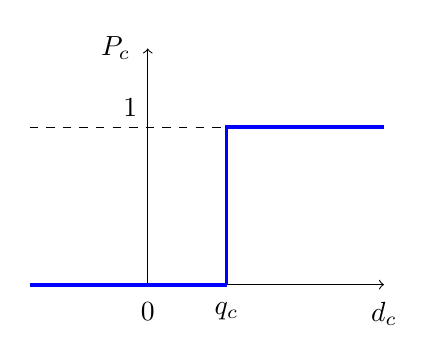
\begin{tikzpicture}
    \draw[->] (-1.5,0) -- (3,0);
    \draw (3,0) node[below=0.1cm] {$d_c$};
    \draw [->] (0,0) -- (0,3);
    \draw (0,3) node[left=0.1cm] {$P_c$};
    \draw (0,0) node[below=0.1cm] {$0$};
    \draw[dashed] (-1.5,2) -- (3,2);
    \draw[domain=-1.5:1,smooth,variable=\x,blue,line width=0.5mm] plot ({\x}, {0});
    \draw (1,0) node[below=0.1cm] {$q_c$};
    \draw[domain=0:2.025,smooth,variable=\y,blue,line width=0.5mm] plot ({1}, {\y});
    \draw (0,2) node[above left=0.01cm] {$1$};
    \draw[domain=1:3,smooth,variable=\x,blue,line width=0.5mm] plot ({\x}, {2});
    \end{tikzpicture}
    \end{center}
\end{minipage}%
\begin{minipage}{.5\textwidth}
    \begin{equation}
        P_c = \left\{
            \begin{array}{l c c}
                0 & \text{if} & d_{c} \le q_c \\
                1 & \text{if} & q_c < d_c \\
            \end{array}
            \right .
            \label{eq:type2_criterion}
    \end{equation}
\end{minipage}
\caption{Preference function for the quasi-criterion}
\end{figure}
This criterion adds an indifference threshold $q_c$. This means that as long as $d_c$ does not exceeds that threshold the difference will be neglected and the two evaluations will be equally prefered.

\subsubsection{Type 3: the criterion with linear preference}
\begin{figure}[H]
\begin{minipage}{.5\textwidth}
    \begin{center}
    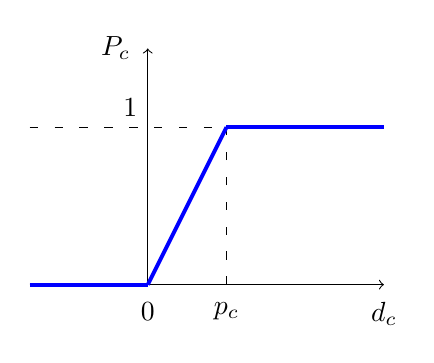
\begin{tikzpicture}
    % axes
    \draw[->] (-1.5,0) -- (3,0);
    \draw (3,0) node[below=0.1cm] {$d_c$};
    \draw [->] (0,0) -- (0,3);
    \draw (0,3) node[left=0.1cm] {$P_c$};
    \draw (0,0) node[below=0.1cm] {$0$};
    % dotted line for 1
    \draw[loosely dashed] (-1.5,2) -- (3,2);
    \draw (0,2) node[above left=0.01cm] {$1$};
    % negatif domain
    \draw[domain=-1.5:0,smooth,variable=\x,blue,line width=0.5mm] plot ({\x}, {0});
    % domain of growth
    \draw (1,0) node[below=0.1cm] {$p_c$};
    \draw[loosely dashed] (1,0) -- (1,2);
    \draw[domain=0:1,smooth,variable=\x,blue,line width=0.5mm] plot ({\x}, {2*(\x)});
    % strict préférence domain
    \draw[domain=1:3,smooth,variable=\x,blue,line width=0.5mm] plot ({\x}, {2});
    \end{tikzpicture}
    \end{center}
\end{minipage}%
\begin{minipage}{.5\textwidth}
    \begin{equation}
        P_c = \left\{
            \begin{array}{l c c}
                0               & \text{if}  & d_{c} \le 0 \\
                \frac{d_c}{p_c} & \text{if}  & 0 < d_c  < p_c \\
                1               & \text{if}  & d_{c} \ge p_c \\
            \end{array}
            \right .
            \label{eq:type3_criterion}
    \end{equation}
\end{minipage}
\caption{Preference function for criterion with linear preferences}
\end{figure}
The preference function for a criterion with linear preferences increases continuously with the difference of the evaluations between $0$ and some threshold $p_c$. If the difference is higher than this threshold, then the alternative with the highest evaluation is strictly prefered over the other.

This preference function is the first one that allows the decision maker to express valued preferences. If the difference of the evaluation lies between $0$ and $p_c$ the preference degree will be between $[0,1]$.

\subsubsection{Type 4: the level-criterion}
\begin{figure}[H]
\begin{minipage}{.5\textwidth}
    \begin{center}
    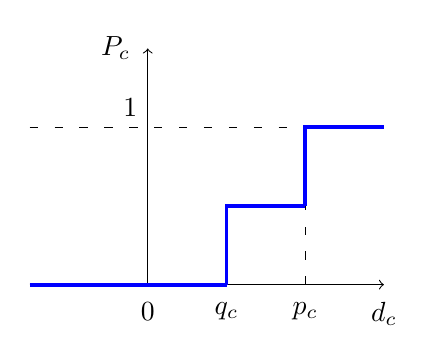
\begin{tikzpicture}
    % axes
    \draw[->] (-1.5,0) -- (3,0);
    \draw (3,0) node[below=0.1cm] {$d_c$};
    \draw [->] (0,0) -- (0,3);
    \draw (0,3) node[left=0.1cm] {$P_c$};
    \draw (0,0) node[below=0.1cm] {$0$};
    % dotted line for 1
    \draw[loosely dashed] (-1.5,2) -- (3,2);
    \draw (0,2) node[above left=0.01cm] {$1$};
    % negatif domain
    \draw[domain=-1.5:1,smooth,variable=\x,blue,line width=0.5mm] plot ({\x}, {0});
    % domain of growth
    \draw (2,0) node[below=0.1cm] {$p_c$};
    \draw[loosely dashed] (2,0) -- (2,2);
    \draw[domain=1:2,smooth,variable=\x,blue,line width=0.5mm] plot ({\x}, {1});
    \draw (1,0) node[below=0.1cm] {$q_c$};
    \draw[domain=0:1.025,smooth,variable=\y,blue,line width=0.5mm] plot ({1}, {\y});
    \draw[domain=1:2.025,smooth,variable=\y,blue,line width=0.5mm] plot ({2}, {\y});
    % strict preferenc domain
    \draw[domain=2:3,smooth,variable=\x,blue,line width=0.5mm] plot ({\x}, {2});
    \end{tikzpicture}
    \end{center}
\end{minipage}%
\begin{minipage}{.5\textwidth}
    \begin{equation}
        P_c = \left\{
            \begin{array}{l c c}
                0 & \text{if}  & d_{c} \le 0 \\
                \frac{1}{2} & \text{if}  & q_c < d_c   \le p_c \\
                1 & \text{if}  &  p_c < d_{c} \\
            \end{array}
            \right .
            \label{eq:type4_criterion}
    \end{equation}
\end{minipage}
\caption{Preference function for level-criterion}
\end{figure}

This criterion uses two parameters, the indifference threshold $q_c$ and the preference threshold $p_c$. If the difference of evaluations lies between these two thresholds, then the preference functions is equal to $0.5$.
This kind of function can be useful for criterions whose evaluations have discrete values (for example a criterion whose values can be ``green'', ``red'', ``blue'').
If the criterion's evaluations can take more than three values, an intuitive generalisation of this preference function with more than three levels can be used.

\subsubsection{Type 5: the criterion with linear preferences and indifference zone} \label{ss:pref_type_5}
\begin{figure}[H]
\begin{minipage}{.4\textwidth}
    \begin{center}
    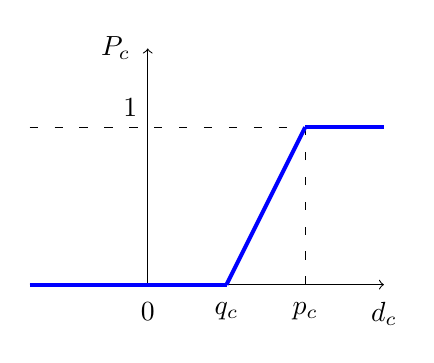
\begin{tikzpicture}
    % axes
    \draw[->] (-1.5,0) -- (3,0);
    \draw (3,0) node[below=0.1cm] {$d_c$};
    \draw [->] (0,0) -- (0,3);
    \draw (0,3) node[left=0.1cm] {$P_c$};
    \draw (0,0) node[below=0.1cm] {$0$};
    % doted line for 1
    \draw[loosely dashed] (-1.5,2) -- (3,2);
    \draw (0,2) node[above left=0.01cm] {$1$};
    % negatif domain
    \draw[domain=-1.5:1,smooth,variable=\x,blue,line width=0.5mm] plot ({\x}, {0});
    % domain of growth
    \draw (2,0) node[below=0.1cm] {$p_c$};
    \draw (1,0) node[below=0.1cm] {$q_c$};
    \draw[loosely dashed] (2,0) -- (2,2);
    \draw[domain=0:1,smooth,variable=\x,blue,line width=0.5mm] plot ({\x+1}, {2*(\x)});
    % strict preferenc domain
    \draw[domain=2:3,smooth,variable=\x,blue,line width=0.5mm] plot ({\x}, {2});
    \end{tikzpicture}
    \end{center}
\end{minipage}%
\begin{minipage}{.6\textwidth}
    \begin{equation}
        P_c = \left\{
            \begin{array}{l l c}
                0                       & \text{if}  & d_{c} \le q_c \\
                \frac{d_c-q_c}{p_c-q_c} & \text{if}  & q_c < d_c  \le p_c \\
                1                       & \text{if}  & p_c < d_c \\
            \end{array}
            \right .
            \label{eq:type5_criterion}
    \end{equation}
\end{minipage}
\caption{ Preference function for the criterion with linear and indifference zone}
\end{figure}

This preference function is a more general version of the Type 3 preference function. Here a parameter $q_c$ can be used to define an indifference threshold.

\subsubsection{Type 6: the gaussian criterion}
\begin{figure}[H]
\begin{minipage}{.4\textwidth}
    \begin{center}
    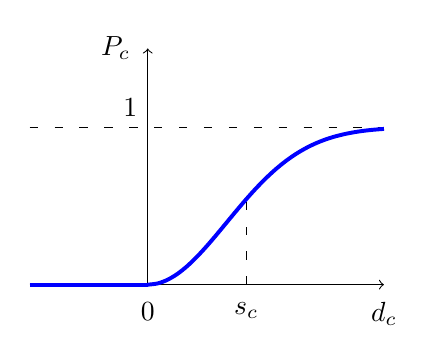
\begin{tikzpicture}
    % axes
    \draw[->] (-1.5,0) -- (3,0);
    \draw (3,0) node[below=0.1cm] {$d_c$};
    \draw [->] (0,0) -- (0,3);
    \draw (0,3) node[left=0.1cm] {$P_c$};
    \draw (0,0) node[below=0.1cm] {$0$};
    % doted line for 1
    \draw[loosely dashed] (-1.5,2) -- (3,2);
    \draw (0,2) node[above left=0.01cm] {$1$};
    % negatif domain
    \draw[domain=-1.5:0,smooth,variable=\x,blue,line width=0.5mm] plot ({\x}, {0});
    % domain of growth
    \draw (1.25,0) node[below=0.1cm] {$s_c$};
    \draw[loosely dashed] (1.25,0) -- (1.25,1.25);
    \draw[domain=0:3,smooth,variable=\x,blue,line width=0.5mm] plot ({\x}, {2-2*exp(-\x*\x/(2)});
    % strict preferenc domain
    %\draw[domain=2:3,smooth,variable=\x,blue,line width=0.5mm] plot ({\x}, {2});
    \end{tikzpicture}
    \end{center}
\end{minipage}%
\begin{minipage}{.6\textwidth}
    \begin{equation}
        P_c = \left\{
            \begin{array}{l l c}
                0                            & \text{if}  & d_{c} \le 0 \\
                1-e^{-d_c^2/2s_c^2} & \text{if}  & 0 < d_c  \\
            \end{array}
            \right .
            \label{eq:type6_criterion}
    \end{equation}
\end{minipage}
\caption{ Preference function for the gaussian criterion}
\end{figure}

This preference function leads to a preference increasing continuously with $d_c$. No threshold parameter is needed for this function but instead, the parameter $s_c$ must be fixed. This parameter indicates the difference $d_c$ needed to have a mean preference (0.39) of the criterion with the highest evaluation over the other.
The advantage of this preference function is that it will never reach 1. There is therefore no threshold of strict preference.


It is important to note that at most two parameters ($q_c$, $p_c$ or $s_c$) must be defined by the decision maker. As each of these parameters have a meaning in the real world, their assignation by the decision maker should not be an insurmountable task \cite{Brans2016}. \\
The choice of these parameters and of the preference functions consists in all the information \textit{within a criterion} \cite{Brans2016} that must be given by the decision maker.
This choice should be done with care as these parameters can have a crucial impact on the final ranking.
For example, choosing indifference thresholds too high for a specific criterion will have as consequence that this criterion will not have much impact as two alternatives will generally be equally preferred regarding to this criterion.
On the other hand, choosing a preference threshold too low will impoverish the preference structure, as alternatives will generally be strictly preferred the ones over the others, and the situation will be similar as when the preference was computed only by taking into account the sign of $d_c$.

\section{Enrichment of the dominance relationship} \label{sec:enrichment_dominance_relation}
\subsection { Global preference index} \label{subsec:global_pref_index}

After having computed the preference degrees for a given pair of alternatives for each criterion, a set of weights $w_c$ must still be defined in order to be able to compute the global preference index $\pi(a_i,a_j)$ of the alternative $a_i$ over the alternative $a_j$.
These weights $w_c$ represent the relative importance of a criterion $c$ compared to the others. The global preference index is given by:

\begin{equation}
    \pi(a_i,a_j) = \sum\limits^k_{c=1} P_c(a_i,a_j)\cdot w_c
    \label{eq:global_preference_index}
\end{equation}

The choice of the different $w_c$ consists in the information \textit{between criteria} \cite{Brans2016} that must be given by the decision maker.
Similarly as for the parameters giving information within a criterion, the choice of the $w_c$ is of the highest importance. For example, a criterion with a weight equal to zero would simply have no influence on the global preference index.

These weights factors must be positive as criteria would have a negative influence otherwise:

\begin{equation}
    w_c \ge 0 \qquad \forall c
    \label{eqn:wc_positif}
\end{equation}

As these parameters only consists of multiplicative constants, there is no inconvenient to choose them normalised:

\begin{equation}
    \sum\limits^k_{c=1} w_c = 1
    \label{eq:normalised_wc}
\end{equation}

Some relations can be deduced from the equations \eqref{eq:generalised_criterion} and \eqref{eq:global_preference_index}:

\begin{equation}
    \pi(a_i,a_i)=0
    \label{eq:pi_self}
\end{equation}
which states that an alternative is not preferred over itself, and
\begin{equation}
    0 \le \pi(a_i, a_j) \le 1
    \label{eq:pi_bounds}
\end{equation}
which holds since the weights are normalised and the $P_c$ are lower or equal to 1.
Furthermore, if $\pi(a_i, a_j)$ is strictly positive, then $\pi(a_j, a_i)$ will be equal to $0$, leading to:
\begin{equation}
    \pi(a_i, a_j) + \pi(a_j, a_i) \le 1
\end{equation}

It should also be clear that \cite{Brans2016}:
\begin{equation}
    \left \{
        \begin{array}[]{l c r}
            \pi(a_i,a_j) \approx 0 & \Leftrightarrow & \text{weak preference of $a_i$ over $a_j$} \\
            \pi(a_i,a_j) \approx 1 & \Leftrightarrow & \text{strong preference of $a_i$ over $a_j$}
        \end{array}
        \right .
    \label{eq:pi_0_1}
\end{equation}

All the pairwise preference indices $\pi(a_i, a_j)$ can be seen as forming an $n \times n$ preference matrix $\Pi$.

\subsection{Outranking flow} \label{sec:outranking_flow}

As just seen here above, $\pi(a_i,a_j)$ gives an indication of how $a_i$ is dominating $a_j$ on all the criterions.
This information is only related to a pair of alternatives and does not give a sufficient indication of the dominance of $a_i$ in the set $A$.

Such as for the \textsc{electre i} method (section \ref{sec:electre}), an outranking graph can be built. However, it will not be a binary outranking graph with arcs going from outranking alternatives to outranked alternatives anymore.
The graph will be a complete digraph on $n$ vertices representing the $n$ possible alternatives. The valued arc going from an alternative $a_i$ to an alternative $a_j$ will be valued $\pi(a_i,a_j)$ \cite{BransVincke85}.
This graph is therefore not a graph directly leading to an ordering, but will, for each pair of alternatives $a_i$ and $a_j$, give a quantified information of how much $a_i$ outranks $a_j$ and vice-versa.

This graph can be used to compute an \textit{outgoing outranking flow} and an \textit{incoming outranking flow} for each alternative \cite{Bertrand2002}. \\
The outgoing flow is given by:
\begin{equation}
    \phi^+(a_i) = \frac{1}{n-1}\sum\limits^n_{j=1} \pi(a_i,a_j)
    \label{eq:outgoing_flow}
\end{equation}
This flow indicates how much alternative $a_i$ is dominating or outranking on average the remaining $n-1$ alternatives. The higher this flow, the more $a_i$ should be preferred by the decision maker.

Similarly, the incoming flow is defined by \cite{Bertrand2002}:
\begin{equation}
    \phi^{-}(a_i) = \frac{1}{n-1}\sum\limits^n_{j=1} \pi(a_j,a_i)
    \label{eq:incoming_flow}
\end{equation}
This flow indicates how much alternative $a_i$ is outranked on average by the $n-1$ other alternatives. The lower this flow, the more alternative $a_i$ should be preferred.

One can see in the expressions of the outranking flows that the summations of the preference index are divided by $n-1$. This is done to ensure that the outranking flows will be lower or equal to $1$ (the summations consist of sums on $n$ terms lower than $1$ from which at least one is null by \eqref{eq:pi_self}).

The netflow score can be obtained by subtracting the incoming flow from the outgoing flow:

\begin{equation}
    \phi(a_i) = \phi^+(a_i) - \phi^-(a_i)
    \label{eq:netflow}
\end{equation}

\section{Decision aid}
\subsection{\textsc{Promethee i}}
To help the decision maker in his task, the \textsc{promethee} methods will rank the alternatives according to their outranking flows.

The two complete preorders ($P^+$,$I^+$) and ($P^-$,$I^-$) obtained with the outranking flows are defined as follow \cite{Bertrand2002}:

\begin{equation}
    \forall a_i, a_j \in A \left \{
        \begin{array}[]{l c c}
            a_iP^+a_j & \Leftrightarrow & \phi^+(a_i) > \phi^+(a_j) \\
            a_iI^+a_j & \Leftrightarrow & \phi^+(a_i) = \phi^+(a_j)
        \end{array}
        \right .
    \label{eq:P1_positif_ranking}
\end{equation}
\begin{equation}
    \forall a_i, a_j \in A \left \{
        \begin{array}[]{l c c}
            a_iP^-a_j & \Leftrightarrow & \phi^-(a_i) < \phi^-(a_j) \\
            a_iI^-a_j & \Leftrightarrow & \phi^-(a_i) = \phi^-(a_j)
        \end{array}
        \right .
    \label{eq:P1_negatif_ranking}
\end{equation}

The \textsc{promethee i} ranking is made by taking the intersection of these two preorders. An alternative $a_i$ is preferred over another alternative $a_j$ according to \mbox{\textsc{promethee i}} if both its outgoing flow and its incoming flow are better (respectively greater and smaller) than the ones of $a_j$. If both the flows are equal for the two alternatives, then the alternatives will be indifferent, and if none of these two cases hold, then the alternatives will be said to be incomparable \cite{Bertrand2002}:


\begin{equation}
  \forall a_i, a_j \in A: \left\{
    \renewcommand{\arraystretch}{1.75}
    \begin{array}{l l}
      a_iPa_j  & \Leftrightarrow \ \ \left\{
          \begin{array}{l }
              a_iP^+a_j \text{ and } a_iP^-a_j \\
              a_iP^+a_j \text{ and } a_iI^-a_j \\
              a_iI^+a_j \text{ and } a_iP^-a_j \\
          \end{array} \right . \\
      a_iIa_j & \Leftrightarrow \qquad a_iI^+a_j \text{ and } a_iI^-a_j \\
      a_iRa_j & \Leftrightarrow \qquad \text{else} \\
    \end{array} \right . \\
    \label{eq:PI_ranking}
\end{equation}



\subsection{\textsc{Promethee ii}} \label{sec:decision_aid_pii}

It can happen that the decision maker wishes to obtain a complete ordering of the alternatives (without any incomparabilities). This can be done using \textsc{promethee ii}. This method builds a ranking based on the net flow score of each alternatives:

\begin{equation}
    \forall a_i,a_j \in A \left \{
        \begin{array}[]{l}
            a_iPa_j \Leftrightarrow \phi(a_i) > \phi(a_j) \\
            a_iIa_j \Leftrightarrow \phi(a_i) = \phi(a_j) \\
        \end{array}
        \right .
    \label{eq:PII_ranking}
\end{equation}

As it can be seen, using \textsc{promethee ii}, two alternatives can be either prefered the one over the other ($P$) either indifferent ($I$). Two alternatives can therefore not be incomparable, leading to a complete preorder of the alternatives.

Furthermore, it should be pointed out that the outgoing, incoming or net flows are not just some artificial and arbitrary constructions made to aggregate the pairwise preferences.
In fact, it can be shown that the net flow score is the centered score that minimizes the sum of the square deviations for the pairwise preferences of the alternatives \cite{mareschal2008rank}.

In other words, if $Q$ is the sum of the square deviations between a centered score $s$ and the pairwise preferences, with $s_i$ being the score of the alternative $a_i$:

\begin{equation}
    Q = \sum\limits_{i=1}^n\sum\limits_{j=1}^n\big[(s_i-s_j) - (\pi(a_i, a_j) - \pi(a_j,a_i))\big]^2
    \label{eqn:square_deviations_sum}
\end{equation}

then $Q$ will be minimal when the score $s_i$ of alternatives are proportionals to their net flows:

\begin{equation}
    s_i = \frac{1}{n}\sum\limits_{j=1}^n (\pi(a_i,a_j)-\pi(a_j,a_i)) = \frac{n-1}{n} \phi(a_i)
    \label{eqn:score_prop_netflow}
\end{equation}

\subsection{Conclusion}

There exist other variations of \textsc{promethee} than the \textsc{promethee i} and \textsc{promethee ii} methods but these will not be detailed here and the interested reader can refer to \cite{Brans2016} for additional information.

There also exists an additional tool, named \textsc{gaia} (Geometrical Analysis for Interactive Assistance), which is, as its name suggests, a tool aimed at performing an interactive visualisation of the data.
Once again, this method will not be detailed here and the interested reader can refer to \cite{Brans2016} or \cite{Bertrand2002} for additional information.

Finally, it should also be noted that part the success of \textsc{promethee} is due to the existence of userfriendly software (such as \textit{D-Sight}) that helps the decision maker in the visualisation of the alternatives and the influence of the different parameters of the method \cite{DeSmet2013}.

A criticism that is often addressed to the \textsc{promethee} methods is that it is subject to the \textit{rank reversal} phenomenon. An introduction to this phenomenon will be presented in the next chapter. Then, two variations of \textsc{promethee ii} which are aimed at reducing these rank reversals will be studied.


\chapter{Rank Reversal}
\label{chap:rank_reversal}

The so called rank reversal phenomenon in a multi-criteria decision aid context is a phenomenon initially highlighted by Belton and Gear in 1983 \cite{belton1983short}\cite{wang2009rank}.

There is not one unique definition of the rank reversal phenomenon but there rather exist several, which however generally share the same idea: ``the relative ordering between two alternatives depends on the presence of one or several other alternatives''. \\
Some of the definitions that can be found in the literature are that the relative position of two alternatives can be influenced by the presence of \cite{Brans2016}:
\begin{itemize}
    \item a non discriminating criterion
    \item a copy of an alternative
    \item a dominated alternative
    \item any other alternative
\end{itemize}

In the rest of this work, unless stated otherwise, we will say that there is a ``rank reversal occurrence'' when the relative ordering between two alternatives is affected by the presence or absence of any third alternative.

This phenomenon can lead to some undesirable consequences. One of these obvious undesirable consequence is highlighted in the following example. \\
Suppose that a municipal administration of a city considers that it is necessary to build a new sports stadium. This could be due to the fact that the existing one is becoming too old or because its capacity is no longer sufficient to host enough supporters.
The municipal administration would therefore organise a competition where architects and entrepreneurs would propose their projects.
The administration could decide to rank all these projects using a multi-criteria decision aid method according to criteria such as the estimated price of the project, the estimated duration of the works, the capacity of the stadium, the capacity of its parking, etc.
The project arriving in first position of the ranking would be selected and built.\\
In such a situation, the possibility of a rank reversal between the first two alternatives would have important consequences as it would influence which stadium would be built, and which group of people would have the right to build it.
There does not seem to be any rational reason why the order of the two first projects should be influenced by the presence of other projects and therefore these kind of rank reversals should be avoided.

In similar situations, it could also be argumented that the multi-criteria decision aid methods which suffers from rank reversal occurrences are vulnerable to ranking manipulations by artificially adding (or removing) some alternatives.

W. De Keyser and P. Peeters \cite{de1996note} were the first to point out that the \textsc{promethee} methods suffer from rank reversal occurrences.

Before going into the specific details of the rank reversal phenomenon in \textsc{promethee}, some characteristics of more general methods based on pairwise comparisons will be given.

\section{Transitivity of preferences and pairwise \\ comparisons}
Some important facts have been highlighted by Mareschal et al. \cite{mareschal2008rank} concerning methods based on the pairwise comparisons of the alternatives.

These facts will be resumed in the rest of this section. First, the notion of \textit{consistent ranking methods based on pairwise comparison} will be defined.
Then, few words will be said about the transitivity of the preferences and finally, it will be shown that consistent ranking methods based on pairwise comparisons with nontransitive preferences matrices suffer from the rank reversal phenomenon \cite{mareschal2008rank}.


\subsection{Ranking methods based on pairwise comparisons}
\label{sec:RBPC}
Let us again consider a multi-criteria decision problem consisting in the ranking of the alternatives from a finite set $A$ of $n$ alternatives which must maximise $k$ evaluation functions.\\
\newpage
If the multi-criteria decision aid method is based on:
\begin{enumerate}
    \item the computation of an $n \times n$ pairwise preferences matrix \textit{Pref} whose elements \textit{pref}$_{ij}$ are global preference indices of the alternative $a_i$ over $a_j$
    \item the exploitation of this matrix to obtain a complete preorder
\end{enumerate}
then it is said to be a \textit{ranking method based on pairwise comparisons} (RBPC) \cite{mareschal2008rank}.

The \textsc{promethee} methods are examples of such methods where the $n \times n$ preferences matrix $\Pi$ consist in the $n \times n$ evaluations of $\pi(a_i, a_j)$ for all $a_i, a_j$ in $A$.

Furthermore, a ranking method based on pairwise comparisons is said to be \textit{consistent} if the ordering obtained with its application on a set of two alternatives is consistent with the $2 \times 2$ preferences matrix.\\
This means that if a consistent ranking method based on pairwise comparisons is applied on a set of two alternatives $a_i$ and $a_j$, with $a_i$ pairwise preferred over $a_j$ (\textit{pref}$_{ij} > $\textit{pref}$_{ji}$) then $a_i$ should be ranked before $a_j$ \cite{mareschal2008rank}.
This property seems rather intuitive and necessary for any ranking method based on pairwise comparisons.

By remembering how the outranking flow is computed in \textsc{promethee} (section \ref{sec:outranking_flow}), one can easily see that it will be consistent with any $2\times 2$ preferences matrix $\Pi$. 
This means that \textsc{promethee} is a consistent ranking method based on pairwise comparisons.
It should however be noted that the ranking obtained with a larger set of alternatives will not necessarily respect all the pairwise preferences anymore. 

As already announced, such methods with nontransitive preferences matrix are susceptible to suffer from the rank reversal phenomenon.
One could therefore wonder why these preferences matrix could be nontransitive.
Some insights into the transitive nature of the preferences will therefore be given in the next section.
% \subsection{Rank reversal in consistent RBPC with intransitive preferences matrix}
% If a multi-criteria method is based on pairwise comparisons, is consistent and is applied on a preferences matrix that is not transitive, then the rank reversals are unavoidable
% One could object that the preferences matrix should be transitive.
%

\subsection{Transitivity of the preferences}
In a mono-criterion context, with a criterion $f(.)$ which must be maximized, the preference relation $P$ of the natural dominance relation is trivially transitive:
\begin{equation}
    \forall a_i, a_j, a_k \in A: \left \{
        \begin{array}{l}
            a_iPa_j \Rightarrow f(a_i) > f(a_j) \\
            a_jPa_k \Rightarrow f(a_j) > f(a_k)
        \end{array} \right .
        \Rightarrow f(a_i) > f(a_k) \Rightarrow a_iPa_k
    \label{eqn:transitivity_preference_monocriterion}
\end{equation}

In a similar way, one could see that the indifference relation is also transitive.

A slightly more elaborated dominance relation can be defined by introducing an indifference threshold $q$:

\begin{equation}
    \forall a_i, a_j \in A: \left\{
        \begin{array}[]{l c c c c}
            f(a_i)  >  f(a_j) + q           &\Leftrightarrow & a_iPa_j \\
            \mid f(a_i) - f(a_j) \mid  \leq  q  &\Leftrightarrow & a_iIa_j \\
            f(a_i)  <  f(a_j)  -q             &\Leftrightarrow & a_jPa_i \\
        \end{array}
        \right .
    \label{eq:dominance_relation_monocriterion_ind_threshold}
\end{equation}

This dominance relation defines a \textit{semiorder} \cite{Vin92}. The preference relation $P$ is still transitive but the indifference $I$ relation is not transitive anymore.
\begin{equation}
    \begin{split}
    \forall a_i, a_j, a_k \in A: \left \{
        \begin{array}{l}
            a_iPa_j \Rightarrow f(a_i) > f(a_j)+q \\
            a_jPa_k \Rightarrow f(a_j) > f(a_k)+q
        \end{array} \right . \\
        \Rightarrow f(a_i) > f(a_k)+q \Rightarrow a_iPa_k
    \end{split}
    \label{eqn:transitivity_preference_monocriterion_indiff_threshold}
\end{equation}
The semiorder dominance structure has been introduced by Luce in \cite{Luce1956} as a way to represent the human preference model (preference and indifference) without relying on the assumption that the indifference relation is transitive.
This hypothesis is justified between others by the fact that a human being cannot discriminate between two evaluations if these are to close one to another. \\
Luce gives the example of 401 numbered cups of coffee where each cup of coffee $i$ would contain $\big( 1+ \frac{i}{100} \big) x$ grams of sugar, with $i=1\dots401$ and $x$ being the weight in grams of a cube of sugar.
When asking to someone to taste any cups $i$ and $i+1$, he will obviously not taste any difference.
On the other hand, when asking to someone to taste the first and the last cup, it is highly probable that he will taste a difference \cite{Luce1956}.

Tversky goes a step further and shows that when considering a multi-criteria context, even the preference relation should not be considered as being necessarily transitive \cite{tversky1969}.
Tversky motivate his statement with the following example.

Consider a decision maker $D$ which must hire one of three possible candidates. The candidates are evaluated according to two criteria: \textit{intelligence} and \textit{experience}. The evaluations of the different candidates can be seen in Table \ref{tbl:tversky_non_transitive_preferences}.


\begin{table}[h]
\center
\begin{tabular}{ l c c c }
    \toprule
     Candidates & & Intelligence   & Experience  \\
     \cmidrule(rl){1-1}   \cmidrule{3-4}
      $x$  & & $2\varepsilon$       & $6\varepsilon$              \\
      $y$  & & $3\varepsilon$       & $4\varepsilon$            \\
      $z$  & & $4\varepsilon$       & $2\varepsilon$            \\
    \bottomrule
\end{tabular}
\caption{Evaluation table of Tversky's example \cite{tversky1969}}
\label{tbl:tversky_non_transitive_preferences}
\end{table}

The evaluations represent some dimensionless scores according to the corresponding criteria with $\varepsilon$ being a constant.

Suppose $D$ values the intelligence more than the experience.
He could therefore adopt the following strategy: 
\begin{itemize}
    \item If a candidate $c_i$ is considered by the decision maker $D$ as more intelligent than a candidate $c_j$, then candidate $c_i$ will be preferred over $c_j$.
    \item If two candidates $c_i$ and $c_j$ are both considered by $D$ as being equally intelligent, then the one with the most experience will be preferred.
\end{itemize}

Now suppose also that $D$ does not find that a difference of score smaller or equal to $\varepsilon$ for the intelligence criterion is enough to be significative (this can be due to the fact that the tests are not precise enough, or simply because $D$ does not care about too small differences).
The ranking of the candidates, based on the intelligence criterion only, will therefore lead to a semiorder structure (as the ones introduced by Luce).\\

This has for consequence that the candidate $y$ is considered by $D$ as being equally intelligent to both the two other candidates, but candidates $x$ and $z$ are not considered as equally intelligent ($z$ being considered more intelligent than $x$).
Since $y$ is considered as equally intelligent as $x$ and $z$, the preference between these pairs will depend on the experience of the candidates.

By defining ($I_{int}, P_{int}$) and ($I_{exp}, P_{exp}$) the indifference and preference relations respectively on the intelligence and experience criterion only, the following preference relations are obtained:
\begin{equation}
    \begin{split}
     \left \{
        \begin{array}{l l}
            yI_{int}z \ \land \ yP_{exp}z \ & \Rightarrow yPz \\
            yI_{int}x \ \land \ xP_{exp}y \ & \Rightarrow xPy \\
            zP_{int}x                 & \Rightarrow zPx
        \end{array} \right . \\
    \end{split}
    \label{eqn:candidates_nontransitive_dominance_rel}
\end{equation}

These considerations will lead to the preferences matrix represented in Figure \ref{fig:untransitive_matrix}.

\begin{figure}[h]
\begin{minipage}{.5\textwidth}
    \begin{equation*}
        P   = \bordermatrix{~ & x    & y    & z   \cr
                            x & 0    & 1    & 0   \cr
                            y & 0    & 0    & 1   \cr
                            z & 1    & 0    & 0   \cr}
        \label{eq:transitive_pref_example}
    \end{equation*}
\end{minipage}
\begin{minipage}{.5\textwidth}
    \begin{center}
     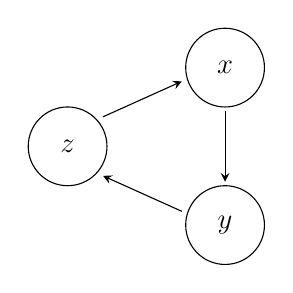
\begin{tikzpicture}[scale=0.5, transform shape]
        % before suppression of alternative
        \draw (4,-2) circle (1) ;
        \draw (4,-2) node{\huge{$y$}};
        \draw (4,2) circle (1) ;
        \draw (4,2) node{\huge{$x$}};
        \draw (0,0) circle (1) ;
        \draw (0,0) node{\huge{$z$}};
        \draw [>=stealth,->] (0.90,0.75) -- (2.90,1.65);
        \draw [>=stealth,->] (2.90,-1.65)-- (0.90,-0.75) ;
        \draw [>=stealth,->] (4,0.9)    -- (4,-0.9) ;
        %\draw [>=stealth,->] (1,2.25) -- (3,3.75);
        % after deletion of a2
        \end{tikzpicture}
   \end{center}
\end{minipage}%
\caption{Example of non transitive preferences matrix and its graphical representation} \label{fig:untransitive_matrix}
\end{figure}

Unlike with the pairwise preferences matrices $\Pi$ of the \textsc{promethee} methods whose elements are valued between $0$ and $1$ and represent the strength with which an element is pairwise preferred over another, this matrix is binary and indicates if an alternative is preferred over another, without giving any indication about the strength of the preference.

It can be seen from this example, that the pairwise preferences of a decision maker which seems to use only reasonable assumptions can be nontransitive.

It will now be shown that any ranking method based on pairwise comparisons which is consistent and uses a nontransitive preferences matrix must suffer from the rank reversal phenomenon.

\subsection{Rank reversal occurrences in consistent RBPC with nontransitive preferences}

To demonstrate that rank reversal occurrences are unavoidable in such conditions, we will consider the problem of having to rank the three candidates presented in the previous section. \\
The considered ranking method will therefore have to aggregate the nontransitive preferences in one global ranking, as shown in Figure \ref{fig:aggregating_nontrans}.
\vskip 0.15cm

\begin{figure}[h]
    \centering
    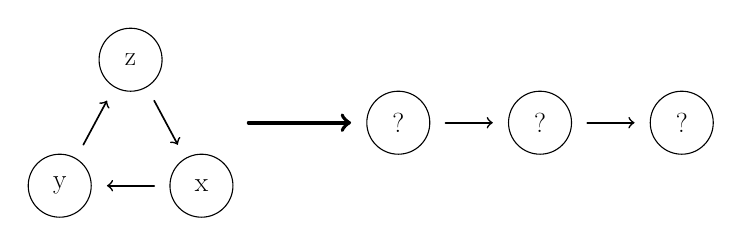
\begin{tikzpicture}[scale=0.4, transform shape, line cap=round,x=1.0cm,y=1.0cm]
        %\clip(-7.7,-4.66543927909192) rectangle (6.858736141587812,4.56639472090804);
        \draw(-1.75,-2.) circle (1.cm) ;  %x
        \draw(-6.25,-2.) circle (1.cm);   %y
        \draw(-4.,2.) circle (1.cm);    %z
        \draw [->,line width=0.6pt] (-5.5,-0.70) -- (-4.75,0.7);     % ab
        \draw [->,line width=0.6pt] (-3.25,0.7) -- (-2.50,-0.700);        % bc
        \draw [->,line width=0.6pt] (-3.25, -2) -- (-4.75, -2);
        \draw(9.,0) circle (1.cm)   ;
        \draw(4.5,0.) circle (1.cm) ;
        \draw(13.5,0.) circle (1.cm);
        \draw [->,line width=0.6pt] (10.5,-0.) -- (12,0.); %23
        \draw [->,line width=0.6pt] (6.,0) -- (7.5,0.);         %12
        \draw [->,line width=1.4pt] (-0.25,0.) -- (3.,0.);
        \draw (9.,0) node {\Huge ?};  %2
        \draw (4.5,0) node {\Huge ?};    %1
        \draw (13.5,0.) node {\Huge ?}; %3
        \draw (-6.25,-2.) node[] {\Huge y};
        \draw (-4.,2.) node[] {\Huge z};
        \draw (-1.75,-2.) node[] {\Huge x};
    \end{tikzpicture}
    \caption{Aggregating non transitive preferences in a ranking} \label{fig:aggregating_nontrans}
\end{figure}

Since the method is considered to be consistent by hypothesis, if one alternative is removed, the ranking obtained by applying the method on the remaining alternatives must respect the pairwise preferences of these alternatives (since the method is applied on only two alternatives).
These conditions are shown in the Figure \ref{fig:consistent_rankings}.

\vskip 0.15cm
\begin{figure}[h]
    \begin{minipage}{0.3\textwidth}
        \centering
        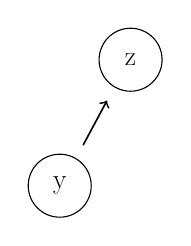
\begin{tikzpicture}[scale=0.4, transform shape, line cap=round,x=1.0cm,y=1.0cm]
            \draw(-6.25,-2.) circle (1.cm);   %a
            \draw(-4.,2.) circle (1.cm);    %b
            \draw [->,line width=0.6pt] (-5.5,-0.70) -- (-4.75,0.7);     % ab
            \draw (-6.25,-2.) node[] {\Huge y};
            \draw (-4.,2.) node[] {\Huge z};
        \end{tikzpicture}
    \end{minipage}
    \begin{minipage}{0.3\textwidth}
        \centering
            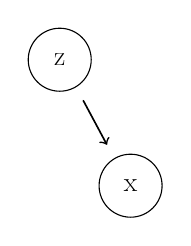
\begin{tikzpicture}[scale=0.4, transform shape, line cap=round,x=1.0cm,y=1.0cm]
            %\clip(-7.7,-4.66543927909192) rectangle (6.858736141587812,4.56639472090804);
            \draw(-1.75,-2.) circle (1.cm);  %c
            \draw(-4.,2.) circle (1.cm);    %b
            \draw [->,line width=0.6pt] (-3.25,0.7) -- (-2.50,-0.700);        % bc
            \draw (-4.,2.) node[] {\Huge z};
            \draw (-1.75,-2.) node[] {\Huge x};
            \end{tikzpicture}
    \end{minipage}
    \begin{minipage}{0.3\textwidth}
        \centering
            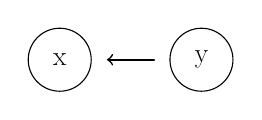
\begin{tikzpicture}[scale=0.4, transform shape, line cap=round,x=1.0cm,y=1.0cm]
            %\clip(-7.7,-4.66543927909192) rectangle (6.858736141587812,4.56639472090804);
            \draw(-1.75,-2.) circle (1.cm);  %c
            \draw(-6.25,-2.) circle (1.cm);   %a
            \draw [->,line width=0.6pt] (-3.25, -2) -- (-4.75, -2);
            \draw (-6.25,-2.) node[] {\Huge x};
            \draw (-1.75,-2.) node[] {\Huge y};
            \end{tikzpicture}
    \end{minipage}
    \caption{Consistent rankings when only two candidates are considered} \label{fig:consistent_rankings}
\end{figure}

It should be quite obvious that it is not possible to find any complete ranking that satisfies these three conditions.
Therefore, whatever the ranking is, it will lead to some rank reversal occurrence when one of the alternatives is removed.\\
The reasoning here above has been done for three alternatives but it remains valid for any set of alternatives where the pairwise preferences between these alternatives form a cycle (such as in figure \ref{fig:untransitive_matrix}).
We can therefore conclude that the rankings obtained with \textsc{promethee} on a set of alternatives, from which a subset have nontransitive pairwise preferences, will inevitably suffer from rank reversal occurrences.

However, this is not the only characterization that can be done concerning the possibility of occurrence of rank reversals in the \textsc{promethee} methods.
The next section will address the possibility of rank reversal occurrences between alternatives dominating each other and the impact of the differences of net flows of two alternatives on their possibility to reverse their ranks. % between alternatives whose net flows are ``distant enough''.


\section{Some results about the rank reversal \\ phenomenon in the \textsc{promethee} methods}

\subsection{Respect of the natural dominance relation} \label{sec:pii_respect_dominance}

An alternative which is at least as good as another alternative on all the criteria and strictly better on at least one criteria is said to dominate this other alternative (see section \ref{sec:multi_criteria_dominance_rel}).
There is obviously no reason why an alternative which is dominated by another should be ranked before this other which would be a violation of the natural dominance relation.
It is therefore reasonable to hope that any ranking method will respect it.\\
This also means that there should not be any strict rank reversal between dominated and dominant alternatives (the dominated alternatives could however become indifferent to the dominant ones under some particular circumstances).

It will be shown here under that the \textsc{promethee} methods respect the dominance relation \cite{DecisionEng} and do not suffer from these kind of rank reversals.

% Assume a finite set $A$ of $n$ alternatives that must maximise a set of $k$ evaluations functions ($f_c(.)$). 
It will be shown that if alternative $a_i$ is dominating alternative $a_j$, then its netflow can not be lower that the one of $a_j$:

\begin{equation}
    \begin{split}
     \left \{
        \begin{array}{l l}
            \forall c=1,\dots, k \ :\qquad & f_c(a_i) \ge f_c(a_j) \\
            \exists h \in \{1,\dots,k\}: \qquad & f_c(a_i) > f_c(a_j)
        \end{array} \right .
        \Rightarrow \phi(a_i) \ge \phi(a_j)
    \end{split}
    \label{eqn:ai_dominates_aj}
\end{equation}

Since $a_i$ is dominating $a_j$, and the preference functions $P_c$ are nondecreasing, we can see that $\pi(a_i,b) \ge \pi(a_j,b)$ for any $b$ in $A$:
\begin{align}
    \begin{split}
        \pi(a_i, b) = \sum\limits^k_{c=1} w_c \cdot P_c(a_i,b)
                    \ge \sum\limits^k_{c=1} w_c \cdot P_c(a_j,b)
                    = \pi(a_j, b)
    \end{split}
    \label{eqn:pi_aib_ge_pi_ajb}
\end{align}

A similar reasoning can be applied to see that $\pi(b,a_i) \le \pi(b, a_j)$.

Therefore we can conclude that:
\begin{align}
    \begin{split}
    \phi(a_i) & = \phi^+(a_i) - \phi^-(a_i) \\
              & = \frac{1}{n-1}\sum\limits_{b\in A} \pi(a_i,b) - \frac{1}{n-1}\sum\limits_{b\in A} \pi(b, a_i)\\
              & \ge \frac{1}{n-1}\sum\limits_{b\in A} \pi(a_j,b) - \frac{1}{n-1}\sum\limits_{b\in A} \pi(b, a_j) \\
              & \ge \phi(a_j)
    \end{split}
    \label{eqn:dominance_demo_phi_ai}
\end{align}

Showing that the dominance relation is respected.

\subsection{Rank reversal and net flow differences}

Having alternatives dominating each other is not the only situation under which rank reversal cannot occur in the \textsc{promethee} methods.
Indeed, rank reversal can occur only between alternatives whose net flows difference is lower than a given limit.

Here under, an initial bound on the net flow difference between two alternatives will be shown under which rank reversal cannot occur when one alternative is removed in \textsc{promethee ii} \cite{DecisionEng}.

% Suppose a set of alternatives $A$ from which an alternative $x$ is removed. The resulting set will be noted $A^{\prime}$. The net flow of an alternative $a_i$ in the new set is given by:
Suppose that alternative $x$ is removed from the set of alternatives $A$. The resulting set will be noted $A^{\prime}$. The net flow of an alternative $a_i$ in the new set is given by:
\begin{align}
    \begin{split}
        \phi^{\prime}(a_i) & =
            \frac{1}{n-2}\sum\limits_{b\in A^{\prime}} (\pi(a_i,b) - \pi(b, a_i)) \\
            & = \frac{1}{n-2}\sum\limits_{b\in A} (\pi(a_i,b) - \pi(b, a_i)) - \frac{1}{n-2}(\pi(a_i,x) - \pi(x,a_i))\\
            &= \frac{n-1}{n-2}\phi(a_i) - \frac{1}{n-2}(\pi(a_i,x) - \pi(x,a_i))\\
    \end{split}
    \label{eqn:phi_a_prime_using_phi_a}
\end{align}

Using the same reasoning for an alternative $a_j$, we can express the net flow difference between the two alternatives in the set $A^{\prime}$ according to their net flow difference in $A$:
\begin{align}
    \begin{split}
        \phi^{\prime}(a_i) - \phi^{\prime}(a_j)
             = & \frac{n-1}{n-2}(\phi(a_i) - \phi(a_j)) \\
                & - \frac{1}{n-2}(\pi(a_i,x) - \pi(x,a_i) - \pi(a_j,x) + \pi(x, a_j))\\
    \end{split}
    \label{eqn_phi_diff_prime_using_phi_diff}
\end{align}

If we suppose that $a_i$ was initially ranked before $a_j$ ($\phi(a_i) - \phi(a_j)> 0$), there will be no rank reversal ($\phi^{\prime}(a_i) - \phi^{\prime}(a_j)> 0$) only if:
\begin{align}
        (n-1)(\phi(a_i) - \phi(a_j) > (\pi(a_i,x) - \pi(x,a_i) - \pi(a_j,x) + \pi(x, a_j))
    \label{eqn:no_rr_phi_condition_using_x}
\end{align}

By remembering that $\pi(a_{\alpha}, a_{\beta})$ can only take values between zero and one (see equation \ref{eq:pi_bounds} in section \ref{subsec:global_pref_index}) we can conclude that there cannot be any rank reversal between $a_i$ and $a_j$ when an alternative is removed if their net flow difference is greater than:
\begin{align}
    \begin{split}
        (n-1)(\phi(a_i) - \phi(a_j) & > (1 - 0 - 0 + 1) \\
        \phi(a_i) - \phi(a_j) & > \frac{2}{n-1}
    \end{split}
    \label{eqn:no_rr_condition}
\end{align}

This bound, which is only valid when one alternative is removed, can however be generalized to the cases where $N$ alternatives are removed:
\begin{align}
    \phi(a_i) - \phi(a_j) > \frac{2N}{n-1}
    \label{eqn:no_rr_generalization}
\end{align}

However, this first bound is quite weak and not really often applicable.
A reinforcement of this bound has been given in \cite{Verly2013} where it is shown that the removal of one alternative cannot cause any rank reversal between alternatives which's net flow difference is greater than:
\begin{align}
    \phi(a_i) - \phi(a_j) > \frac{2}{n-1}\cdot W_{ij}
    \label{eqn:rr_bound_verly}
\end{align}

where:
\begin{align}
    W_{ij} = \sum\limits_{c=1, f_c(a_i) \ge f_c(a_j)}^k w_c
    \label{eqn:Wij}
\end{align}
represents the total weight of the coalition of criteria where $a_i$ is as least as good as $a_j$ \cite{Verly2013}.

\section{Comments about the rank reversal phenomenon and conclusion}

As it has been seen, the rank reversal problem is far from being a trivial one.
There seems to be situations where the rank reversal phenomenon could be seen as reasonable (with nontransitive preferences) but there are also cases where it should be avoided (such as in the example of the sport stadium). 

It should also be noted that this phenomenon is not restricted to the area of multi-criteria decision aid.
Indeed, it had already been highlighted earlier in social choice theory, and more particularly in Kenneth Arrow's famous impossibility theorem \cite{arrow1950difficulty} and its condition of \textit{Independence of irrelevant alternatives}.

The problematic of rank reversal in the multi-criteria decision aid domain has already been addressed and is still addressed by numerous authors (some of them have already been mentioned in this chapter) and it is important to point out that the issue of the legitimacy of this phenomenon has not been settled yet.

% The rest of this work is not aimed at answering to the question of the legitimacy of this phenomenon.
The rest of this work is not aimed at answering this question. 
It rather starts from the ascertainment that rank reversals occurs in the \textsc{promethee} methods, and proposes an investigation of two approaches aimed at reducing or suppressing them.

The first approach is called \textsc{robust promethee} and will be described in the next chapter.
It is based on the repetition of \textsc{promethee ii} a great number of times on small subsets of alternatives chosen at random. 

The second approach is called \textsc{referenced promethee}. It is based on the application, for each of the considered alternatives, of \textsc{promethee ii} on a set constituted of this alternative and of predefined reference profiles. This method, by construction, does not suffer from rank reversals.

These two methods unfortunately do not provide solutions without any cost. The distinctive features of these methods, as well as the additional information needed from the decision maker for each of them will be detailed in their corresponding chapters.





\chapter{The \textsc{robust promethee} method} \label{sec:Robust_Promethee}
\label{chap:robst}

\begin{sloppypar}
\textsc{robust promethee} is a multi-criteria decision aid method based on \mbox{\textsc{promethee ii}}.
%Such as \textsc{promethee ii}, it must be applied on a finite set $A$ of $n$ alternatives, with a finite family of $k$ evaluation functions $f_c(.)$ and produces a complete ranking.
It has originally been proposed by De Smet in \cite{RobPII}.
\end{sloppypar}


% \begin{sloppypar}
As indicated by its name, it is aimed to be more robust than \mbox{\textsc{promethee ii}} (with respect to rank reversal occurrences). 
Such as for the notion of rank reversals, the notion of robustness is not univocally defined (see \cite{Roy2010629}, \cite{Hites2006322} and \cite{barrico2006robustness}).
In this work, the following definition of a robust solution will be used:
% \end{sloppypar}
\begin{quote}
    \textit{
    ``a robust solution shall behave well in (slightly) different conditions, meaning that it is as much as possible immune to small changes in the conditions it was designed for.''} \cite{barrico2006robustness}
\end{quote}

More specifically, it is hoped that \textsc{robust promethee} will produce rankings more robust with respect to the sets of alternatives on which it is applied.
This means that if the set of alternatives is slightly changed (in particular if one alternative is added or removed), then the ranking should remain globally the same (excepted for the added alternative).
If this method is effectively robust in this regard, then it should less suffer from the rank reversal phenomenon. 
This last assertion will be studied in this chapter.

The idea used to make \textsc{robust promethee} robust consists in repeating \textsc{promethee ii}, a certain amount of times, on different samplings of the alternatives. 
These samplings (or subsets) consist of a fixed quantity of alternatives taken uniformly at random from $A$ (without replacements). The final ranking will then be built using all the sub-rankings obtained with the different samplings. 

\newpage 

\textsc{robust promethee} is a method based on pairwise comparisons (see section \ref{sec:RBPC}).
The rankings obtained during the iterations are used to compute a pairwise probability matrix $P$ which has the role of the $n \times n$ matrix of pairwise preferences:
% purpose would be similar to the purpose of the pairwise preferences matrix $\Pi$ of the classic \textsc{promethee} methods:
\begin{itemize}
    \item The elements $p_{ij}$ are computed as the probability that the alternative $a_i$ would be ranked before the alternative $a_j$ in one of the random subsets.
    \item Once the iterations are completed, the alternatives would be ranked according to their net flow scores computed on the pairwise probability matrix.
\end{itemize}

These elements $p_{ij}$ are therefore indicators that are used to asses the probability that alternative $a_i$ should be ranked before $a_j$ by the decision maker, independently of the subsets used.
Therefore, just as the net flow score computed on the $\Pi$ matrix, is the centered score that minimizes the sum of the square deviations for the pairwise preferences of the alternatives (see section \ref{sec:decision_aid_pii}), \textsc{robust promethee}'s net flow score will be a score that minimizes the sum of the square deviations for the pairwise probabilities of being ranked before the other alternatives.

This chapter is organized as follow.
First, a more detailed description of the algorithm of this method will be given, then, the first empirical results will be presented, and finally, some of its mathematical properties will be studied.

\section{The \textsc{robust promethee} algorithm}

\textsc{robust promethee} is based on the repetition of \textsc{promethee ii} on different samplings of the alternatives.
% In the rest of this work we will consider, as usual, a set $A$ of $n$ alternatives which must maximise $k$ evaluation functions $f_c(.)$.
We will denote with $R$ this quantity of repetitions and $m$ the size of the samplings (or subsets).
The value of $m$ is supposed to be constant. 

Mathematically speaking, the method can easily be defined with the help of the two following families of functions:

\begin{equation}
  \label{eqn:ar}
  \begin{split}
      A_{mr}(a_{i}) = \left\{
    \begin{array}{l l}
        1 & \ \text{if $a_{i}$ is in the $m$ selected alternatives at iteration $r$}\\
        0 & \ \text{else}\\
    \end{array} \right .
    \end{split}
\end{equation}
\begin{equation}
  \label{eqn:beats_r}
  Beats_{r}( a_{i}, a_{j}) = \left\{
    \begin{array}{l l}
      1 &           \ \text{if $a_{i}$ is ranked before $a_{j}$ at the iteration $r$}\\
      \frac{1}{2} & \ \text{if $a_{i}$ and $a_{j}$ have the same ranking}\\
      0 &           \ \text{else}\\
    \end{array} \right .
\end{equation}

The first ones, $A_{mr}(a_{i})$, simply serve as indicators of whether a given alternative is selected at the $r$th iteration of the procedure. \\
The other ones, $Beats_r(a_{i}, a_{j})$, indicate if a specific alternative is ranked before another specific alternative.
In other words, these functions indicate whether the alternative $a_i$ has beaten alternative $a_{j}$.
If one of these two alternatives was not selected at the $r$th iteration, then the function will be equal to zero.

With the help of these two family of functions, the elements of the probability matrix can be assessed as follows:

\begin{equation}
    \label{eqn:pij}
    p_{ij} = \frac{\sum\limits_{r=1}^R Beats_r(i,j)}{\sum\limits_{r=1}^R A_{mr}(i)\cdot A_{mr}(j)}
\end{equation}

Finally, the net flow is computed on the preference matrix. This net flow will be denoted further as robust flow ($\phi_{rob}$) to prevent any ambiguities.

\begin{equation}
    \phi_{rob}(a_i) = \frac{1}{n-1}\sum\limits^n_{j=1} (p_{ij} - p_{ji})
    \label{eqn:rob_phi}
\end{equation}

However, this method could in practice be implemented in a computationally more efficient manner. A proposition of a more efficient algorithm can be found in appendix \ref{app:rob_promethee_algorithm}.

In the following section, the first empirical results will be analysed.

\section{First empirical results} \label{sec:Robust_Promethee_empirical_results}

Some first results of \textsc{robust promethee} have been given in \cite{RobPII} where it has been applied on a simplified version of the \textsc{hdi} dataset \cite{HDI}.
This simplified version of the dataset consists in a subset of the twenty best ranked countries which are evaluated using only two criteria.

These first results, obtained with $R$ equal to $10.000$ and $m$ equal to $5$, were quite encouraging and lead to two observations:
\begin{itemize}
    \item the ranking obtained with \textsc{robust promethee} is quite close with the one obtained with \textsc{promethee ii} (Kendall rank correlation coefficient between the two rankings is equal to $0.968$).
    \item the use of \textsc{robust promethee}  did not lead to any rank reversal (instead of twenty when using the classical \textsc{promethee ii} method).
\end{itemize}

To compute the number of rank reversal occurrences caused by a method, the following procedure is applied.
First, an initial ranking $\mathcal{R}$ is built using the set $A$ of $n$ alternatives.
%First, the studied method is applied on the initial set $A$ of $n$ alternatives and an initial ranking $\mathcal{R}$ is built.
Then, one alternative $a_x$ is removed from this set (and from the initial ranking) and a new ranking $\mathcal{R}^\prime$ is computed.
The minimal number of pairwise inversions that are needed to obtain the original ranking $(\mathcal{R} -{a_x})$ from the new one $(\mathcal{R}^\prime)$ is the number of rank reversal caused by the removal of $a_x$.
This operation is repeated for each $a_x$ in $A$. \\
The total number of rank reversals obtained with the method is equal to the sum of the rank reversals obtained for all the iterations of this procedure.

In the rest of this section, some further empirical investigation of the \textsc{robust promethee} method will be carried out on the already mentioned \textsc{hdi} data set, as well as on subsets of the \textsc{shanghai} ranking \cite{SHA} and of the \textsc{epi} data set \cite{EPI}.

Some technical details such, as the values of parameters of the \textsc{promethee ii} method $(w_c, f_c(.), p, q)$, will not be detailed in this work but can be found on the \textit{GitHub} repository hosting the code of all the tests performed during this master thesis\cite{Gilles2017}.
However, it should be clear that rankings obtained with \textsc{robust promethee} will only be compared to rankings obtained with \textsc{promethee ii} using the same sets of parameters.
For reasons of ease, all tests are performed with preference functions of type 3 (see section \ref{sec:pref_struct}).

\subsection{Empirical results with the \textsc{hdi} data set}

The numbers of rank reversals caused by the \textsc{robust promethee} method on the \textsc{hdi} data set for different values of $R$ and $m$ are represented in Table \ref{tbl:robust_PII_HDI}.
\begin{table}[h]
    \centering
    \begin{tabular}{C @{\hskip 1cm}C C C C C C C C C C}
        \toprule
    R \backslash m & 3  &   5   &  6    &   7   &  8   &  10   &  15 \\ [7pt]
        \midrule
          500    & 2.2  &  3.85 & 0.3  & 1.55  & 13.9   &  28.9   &  13\\
          1 000  & 0.55 &  0.8  & 0.05 & 0.15  & 11.95  &  24.15  &  10.9\\        
          5 000  & 0    &  0.05 & 0    & 0     & 4.95   &  18.35  &  10.9\\        
          10 000 & 0    &  0    & 0    & 0     & 3.55   &  18     &  8.1 \\        
        \bottomrule
    \end{tabular}
    \captionsetup{width=10cm}
    \caption{Quantity of rank reversals with a subset of 20 alternatives from the \textsc{hdi} data set (average of 20 repetitions).}
    \label{tbl:robust_PII_HDI}
\end{table}

As it has already been stated, the method does not yield any rank reversal for appropriate values of $R$ and $m$. This is a significant improvement since \textsc{promethee ii} yields 20 rank reversals when applied with this data set.
However this number of rank reversals is highly dependent of $R$ and $m$.

First, it can be seen that, up to a certain point, the number of rank reversals decreases as the value of $R$ increases.
This is not surprising and can be intuitively understood.
When performing $R$ iterations, it is as if an sample of size $R$ of all the possible subsets of alternatives $A_m$ was evaluated.
The smaller the sample size is, the higher the variances of it's properties are, and the less the elements $p_{ij}$ of our pairwise probability matrix are significant and stable.
Therefore, the value of $R$ should be chosen large enough.

The effects of the parameter $m$, on the other hand, are not so trivial.
It can be seen that while $R$ is relatively small, the value of $m$ should not be taken neither too small, neither too large, its optimal value being $6$ for this data set.
On the other hand, if $R$ is large enough, the values of $m$ smaller or equal to $7$ all lead to a ranking with no rank reversal occurrence.

\subsection{Empirical results with the \textsc{shanghai} data set}

The numbers of rank reversals caused by \textsc{robust promethee} on a random subset of $20$ alternatives from the \textsc{shanghai} data set for different values of $R$ and $m$ are represented in table \ref{tbl:robust_PII_SHA}.
This set of alternatives consists in six criteria to maximise.

\begin{table}[h]
    \centering
\begin{tabular}{C @{\hskip 1cm}C C C C C C C C C C}
    \toprule
R \backslash m& 4    &   6   &  8    &   9   &  12   &  15   &  18 \\ [7pt]
    \midrule
    1 000    & 53.70 & 21.95 & 14.40 & 12.25 & 14.25 & 14.70 & 12.30 \\
    5 000    & 46.70 & 18.50 & 11.45 & 10.75 & 12.3 & 14.45 & 12.0 \\
    10 000   & 41.20 & 19.05 & 11.40 & 10.25 & 12.15 & 14.15 & 12.0 \\
    20 000   & 40.25 & 19.00 & 11.50 & 10.30 & 12.10 & 14.25 & 12.0 \\        
    \bottomrule
\end{tabular}
\caption{Quantity of rank reversals with a subset of 20 alternatives from the \textsc{shanghai} data set (average of 20 repetitions).}
\label{tbl:robust_PII_SHA}
\end{table}

With this set of alternatives, it is not possible anymore to completely avoid rank reversals. 

\textsc{promethee ii} leads to $14$ rank reversals. The effectiveness in reducing this rank reversal quantity of \textsc{robust promethee} thus highly depends on the value of $m$ used and is limited. 
It can also be seen that the quantity of rank reversal is not monotonically decreasing with the increase of R.

The remaining rank reversals obtained using the optimal value of $m$ ($9$) and a great enough value of $R$ (5000) are further analysed in Table \ref{tbl:robust_PII_SHA_rr_analyse}.

\begin{table}[h]
    \centering
    \begin{tabular}{C C @{\hspace{2em}} C C C C}
\toprule
a_i  & a_j  & \multicolumn{1}{p{1cm}}{\centering Mean\\ \textsc{rob}}  & \multicolumn{1}{p{1.5cm}}{\centering Mean\\ \textsc{pii}} &  \Delta \phi    & \Delta \phi_{rob} \\ [5pt]
\midrule
 10  &    7  &  2.10 &  2  &  0.00770  &  0.01627    \\
 18  &   14  &  0.60 &  0  &  0.00962  &  0.05815    \\
 19  &    2  &  3.00 &  3  &  0.00623  &  0.03515    \\
 10  &    9  &  2.00 &  2  &  0.00722  &  0.03765    \\
  9  &    7  &  3.05 &  7  &  0.00048  &  0.02137    \\
\bottomrule
    \end{tabular}
    \captionsetup{width=10cm}
\caption{Analyse of remaining rank reversals on a subset of 20 alternatives from the \textsc{shanghai} data set, m=9, R=5000, 20 repetitions}
    \label{tbl:robust_PII_SHA_rr_analyse}
\end{table}


The two first columns contain the indices of the alternatives whose rank are reversed during the procedure.
The two next ones contain the number of times these rank reversal happened with the \textsc{robust promethee} and \textsc{promethee ii} methods respectively.

It can be seen that one ``new kind'' of rank reversal is introduced with the use of \textsc{robust promethee} as the alternatives $a_{18}$ and $a_{14}$ can have their rank reversed (which is not the case with \textsc{promethee ii}).
However, this kind of rank reversal does not happen often (only slightly more than once every two executions).

The last columns contain the net flow and robust flow differences between the two concerned alternatives.
It can be observed that the flow differences between the alternatives which suffer from rank reversal are relatively small.

\subsection{Empirical results with the \textsc{epi} data set}

The numbers of rank reversals caused by \textsc{robust promethee} on a subset of the $20$ first alternatives from the \textsc{epi} data set for different values of $R$ and $m$ are represented in table \ref{tbl:robust_PII_EPI}.
This data set consists in nine criteria to maximise.

\begin{table}[!h]
    \centering
    \begin{tabular}{C @{\hskip 1cm}C C C C C C C C C C}
        \toprule
    R \backslash m & 3   &   4   &  7    &   9   &  12   &  14   &  16 & 18 \\ [7pt]
        \midrule
            500  & 49.1  & 63.3  & 31.8  & 22.8  & 10.8  &  9    & 8   & 9.0   \\
          1 000  & 37.5  & 49.9  & 27.2  & 19.4  & 10.5  &  8.7  & 7.8 & 9.0     \\
          5 000  & 19.4  & 38.3  & 25.5  & 20.2  & 11.3  &  9    & 8.7 & 9.0     \\
          8 000  & 18.4  & 34.0  & 25.8  & 19.0  & 11.2  &  9    & 7.8 & 9.0     \\
        \bottomrule
    \end{tabular}
    \captionsetup{width=10cm}
\caption{Quantity of rank reversals with a subset of 20 alternatives from the \textsc{epi} data set (average of 10 repetitions).}
    \label{tbl:robust_PII_EPI}
\end{table}

The use of \textsc{promethee ii} on the same set of alternatives leads to $11$ rank reversals.

The observations that can be done from these results are very similar to the ones done with the \textsc{shanghai} data set.
First, the decrease in the quantity of rank reversal is again relatively small.
Second, the effectiveness of \textsc{robust promethee} on this data set strongly depends on the value of $m$.

On the other hand, the best results are obtained with values of $m$ which are high enough, which is quite different of what had been seen with the \textsc{shanghai} data set and is exactly the opposite of what had been seen with the \textsc{hdi} data set.

Here under, the remaining rank reversals obtained using the optimal value of $m$ ($16$) and a great enough value of $R$ ($5000$) have been further analysed:

\begin{table}[h]
    \centering
    \begin{tabular}{C C @{\hspace{2em}} C C C C}
\toprule
a_i  & a_j  & \multicolumn{1}{p{1cm}}{\centering Mean\\ \textsc{rob}}  & \multicolumn{1}{p{1.5cm}}{\centering Mean\\ \textsc{pii}} &  \Delta \phi    & \Delta \phi_{rob} \\ [5pt]
\midrule
 19  &   18  &  2.0  &  2  &  0.00332  &  0.09299    \\
 18  &   15  &  1.0  &  1  &  0.00399  &  0.13705    \\
 10  &    6  &  1.0  &  0  &  0.00493  &  0.09773    \\
 18  &    4  &  1.0  &  1  &  0.00311  &  0.10381    \\
 19  &   15  &  4.1  &  6  &  0.00067  &  0.04406    \\
 15  &   14  &  1.0  &  1  &  0.00422  &  0.09175    \\
\bottomrule
    \end{tabular}
    \captionsetup{width=10cm}
\caption{Analyse of rank reversals on a subset of 20 alternatives from the \textsc{epi} data set, m=16, R=5000, 10 repetitions}
    \label{tbl:robust_PII_EPI_rr_analyse}
\end{table}

Again, the same remarks as with the \textsc{shanghai} data set can be made:
\begin{itemize}
    \item nearly all rank reversals caused by \textsc{robust promethee} are also caused by the \textsc{promethee ii} method, 
    \item rank reversal occurs only between alternatives having close flows.
\end{itemize}

This last observation is important as it leads to the conjecture that \textsc{robust promethee} will perform better (suffer from fewer rank reversal occurrences) when the alternatives of the problem are sufficiently discriminated.

After having empirically studied the results of the application this method on various data sets of different natures, we will now focus on studying it and more precisely, some of its properties related to the randomness of the selection of the subsets.

\section{Mathematical properties of \textsc{robust promethee}}

So far, it has been observed empirically that \textsc{robust promethee} was producing a ranking quite similar to the \textsc{promethee ii} ranking, that it is more efficient when the alternatives are sufficiently discriminated and when the number of iterations is high enough, and that the optimal size of the subsets is not trivial to determine as it vary according to the set of alternatives on which the method is applied.

In the first part of this section, some lower bound on the number of iterations that are needed to obtain a meaningful probability matrix $P$ (and therefore a meaningful ranking) will be given.
Then it will be shown that, due to the random selection of the subsets and to the presence of rank reversal in \textsc{promethee ii}, \textsc{robust promethee} does not always respect the dominance relation.

\subsection{Pairwise comparisons probability -- lower bound on the number of iterations}

As already stated, the \textsc{robust promethee} ranking is obtained by computing the net flow score of each alternative on the probability matrix $P$.
An element of P, $p_{ij}$, is computed using equation \ref{eqn:pij} and should represent the probability that an alternative $a_i$ should be ranked before an alternative $a_j$.

However, in practice, $p_{ij}$ makes sense only if alternative $a_{i}$ and alternative $a_j$ have been compared pairwise at least once during the \textsc{robust promethee} procedure, i.e.\ when:

\begin{equation}
    \sum\limits_{r=1}^R A_{mr}(i)\cdot A_{mr}(j) \ne 0
    \label{eqn:pij_sens_condition}
\end{equation}

Two upper bounds on the probability that there exist at least two alternatives which have not been compared pairwise during the \textsc{robust promethee} method will be given here under.
These upper bounds on the probability will depend only on the number of alternatives of the problem, the size of the subsets, and the number of iterations of the method.
These bounds will allow us to deduce a lower bound on the values of $R$ and $m$ given a desired upper bound probability that two alternatives have not been compared pairwise, and given a set of alternatives (with fixed size $n$).\\

The number of distinct couples that can be made from the $n$ alternatives of the decision problem is given by:
\begin{equation}
    \label{def:couples}
    N:= C_n^2
\end{equation}
and, at each iteration, we compare $m$ random alternatives pairwise which means that:
\begin{equation}
    \label{def:iterationcouples}
    M:= C_m^2
\end{equation}
distinct couples are evaluated.

To find the desired bound on the probability that there exists a couple of alternatives which has not been evaluated, we will use some known results of the \textit{coupon collector's problem} \cite{Mitzenmacher:2005:PCR:1076315}.

The coupon collector's problem can be described as follow:

\begin{quote}
\textit{
At each iteration $i$, $Di$ balls are picked at random from an urn containing $k$ red balls. These balls are painted in white before being put back in the urn. After how many draws will all the balls be painted in white ?\\}
\end{quote}


It is obvious that this problem can be applied to the one of comparing all alternatives pairwise in the \textsc{robust promethee} method. Instead of having to observe $k$ red balls, there are $N$ couples of alternatives that should be compared and instead of observing $D_i$ balls at iteration $i$, $M$ couples are compared.
However, since we are interested in finding an upper bound of the probability, the assumption will be made that the couples are drawn one at the time which will highly simplify the reasoning.
This assumption is sound since when the couples are drawn $M$ at a time, we have the guarantee that these $M$ couples are distinct one from the other which is not the case otherwise. The upper bound on the probability and the lower bound on the values of $R$ and $m$ that will be found will therefore be higher than the real ones.

We will define:
\begin{description}
\item[$D:=$] the number of random couples needed to observe all the couples at least once.
% \item[$d_i$:= ] the number of random couples needed to observe the $i$th couple after having already observed $(i-1)$ couples.
\end{description}

The probability of finding a new couple after that $(i-1)$ couples have already been found is given by:
\begin{equation}
    \label{eqn:pti}
    p_i = \frac{N - (i-1)}{N}
\end{equation}

% Observing that the variable $d_i$ follows a geometric law, and that
% \begin{equation}
%     D=\sum_i d_i
% \end{equation}
% We can find the expectation and variance of $D$:
The expectation and the variance of $D$ are given by the following relations (see appendix \ref{app:coupon_collector}):
\begin{equation}
    E[D] = N\cdot H_N    \qquad Var[D] \le \frac{\pi ^2N^2}{6}
    \label{eqn:var_exp_D}
\end{equation}
with $H_N$ being the $N$th harmonic number

\subsubsection{Chebyshev Inequality}
Knowing the variance and the expectation of the random variable $D$, a probabilistic bound can be found using Chebyshev's inequality:
\begin{equation}
    \label{eqn:chebshev}
    P[\lvert D - N\cdot H_N\lvert \ge c \frac{\pi N }{\sqrt{6}}] \le \frac{1}{c^2}
\end{equation}

By setting $p = \frac{1}{c^2}$ the desired upper bound probability:
\begin{equation}
    \label{eqn:prob_cheb_with_abs}
    P[\lvert D -N \cdot H_N\lvert \ge \frac{\pi N}{\sqrt{6p}}] \le p
\end{equation}
Since we are only interested to find a bound on the probability that all the couples have not yet been evaluated, the absolute value in the previous equation will be simplified as follow:
\begin{equation}
    \label{eqn:prob_cheb}
    P[D \ge N \cdot H_N +\frac{\pi N}{\sqrt{6p}}] \le p
\end{equation}
Once again, this simplification has for consequence that the bound that will be found on the number of iterations and the size of the subsets is higher than the real one.

Since this bound should be valid after that $R\cdot M$ random couples have been evaluated, we find the following restriction:
\begin{equation}
    \label{prob_bound}
    \begin{split}
    R\cdot M  & \ge N\cdot H_N + \frac{\pi N}{\sqrt{6p}}  \\
        & \Rightarrow \quad P[D \ge R\cdot M] \le p
    \end{split}
\end{equation}

Finally, by replacing $M$ and $N$ by their definitions (\ref{def:couples} and \ref{def:iterationcouples}) we find the desired bound:
\begin{equation}
    \begin{split}
     R\frac{m^2 -m }{2} & \ge \frac{n^2-n}{2}\cdot H_\frac{n^2-n}{2}  + \frac{\pi \frac{n^2-n}{2}}{\sqrt{6p}} \\
     R(m^2 -m) & \ge (n^2-n) H_\frac{n^2-n}{2} + \frac{\pi (n^2-n)}{\sqrt{6p}}
    \end{split}
    \label{eqn:mr_values_cheb_bound}
\end{equation}

\subsubsection{Union bound argument}
Another bound can easily be found simply by making the union bound of the probabilities that one couple has not be evaluated after the evaluation of $c$ random couples.
The probability $P(i,c)$ of not having found a specific couple (called here the $i$th couple) after $c$ random couples have been drawn is lower than:
\begin{equation}
    \begin{split}
    P(i,c) & = (1-\frac{1}{N})^c \\
    & \le e^{\frac{-c}{N}}
    \end{split}
    \label{eqn:bound_p_for_i}
\end{equation}

By making the union of the probabilities for the $N$ couples:
\begin{equation}
    P[D > c] \le N\cdot e^{-\frac{c}{N}}
\end{equation}

This inequality can be justified by the fact that $P[D > c]$ can be seen as the probability that at least one couple has not yet been evaluated after the evaluation of $c$ couples, and by remembering
Boole's inequality: %\cite{SENETA199224}:

\begin{equation}
    P \left( \mathop{\bigcup}_i B_i \right) \le \sum _i P(B_i)
    \label{eqn:Boole_ineq}
\end{equation}
with the $B_i$ forming a set of events.

Setting $p=N\cdot e^{-\frac{c}{N}}$ the desired upper bound probability, the above bound becomes:
\begin{equation}
    P[D \ge N\cdot \ln (\frac{N}{p})] \le p
\end{equation}

Such as for the bound found using Chebyshev's inequality, this bound should be valid after that $R\cdot M$ random couples have been evaluated:
\begin{equation}
    \begin{split}
        R\cdot M & \ge N \cdot \ln (\frac{N}{p}) \\    
        & \Rightarrow \quad P[D \ge R\cdot M] \le p
    \end{split}
    \label{eqn:mr_values_unionprob}
\end{equation}

This restriction can easily be translated in terms of parameters of the \textsc{robust promethee} method ($R$, $m$ and $n$):
\begin{equation}
    R\cdot (m^2-m) \ge (n^2-n) \ln (\frac{n^2-n}{2p})
    \label{}
\end{equation}

More details about the two reasonings here above can be found in \cite{Mitzenmacher:2005:PCR:1076315}.

\subsubsection{Comparison of the bounds}

Since the harmonic number has a logarithmic asymptotic behaviour (but is greater than a logarithm) we can deduce that the bound found using the union bound argument will be tighter than the one found using Chebyshev's inequality.
This statement is confirmed by the Figure \ref{fig:bounds_on_Rm} illustrating the bound on $R$ and $m$ in function of the number of alternatives.

\begin{figure}[!t]
    \centering
    \newlength\figureheight
    \newlength\figurewidth
    \setlength\figureheight{6cm}
    \setlength\figurewidth{6cm}
    % This file was created by matlab2tikz.
%
%The latest updates can be retrieved from
%  http://www.mathworks.com/matlabcentral/fileexchange/22022-matlab2tikz-matlab2tikz
%where you can also make suggestions and rate matlab2tikz.
%
\begin{tikzpicture}

\begin{axis}[%
width=0.976\figurewidth,
height=\figureheight,
at={(0\figurewidth,0\figureheight)},
scale only axis,
unbounded coords=jump,
xmin=0,
xmax=35,
xlabel style={font=\color{white!15!black}},
xlabel={Number of alternatives (n)},
ymin=0,
ymax=25000,
ylabel style={font=\color{white!15!black}},
ylabel={R(m²-m)},
axis background/.style={fill=white},
title style={font=\bfseries, align=center},
title={Lower bound of the Robust Promethee variables\\[1ex]with p=0.01},
xmajorgrids,
ymajorgrids,
legend style={legend cell align=left, align=left, draw=white!15!black}
]
\addplot [color=red]
  table[row sep=crcr]{%
0	0\\
1	0\\
2	27.6509966032373\\
3	87.9529898097119\\
4	183.305979619424\\
5	315.089331111738\\
6	484.311818845429\\
7	691.775994268018\\
8	938.149483072761\\
9	1224.00413988576\\
10	1549.8401775453\\
11	1916.10215648992\\
12	2323.19014433359\\
13	2771.4678190237\\
14	3261.26854061302\\
15	3792.90001921513\\
16	4366.64798135329\\
17	4982.77910233012\\
18	5641.54338838129\\
19	6343.17613821827\\
20	7087.8995775081\\
21	7875.92423519082\\
22	8707.45011329402\\
23	9582.66768959483\\
24	10501.7587835311\\
25	11464.8973091509\\
26	12472.2499339324\\
27	13523.9766585368\\
28	14620.2313296609\\
29	15761.1620959022\\
30	16946.9118147781\\
31	18177.6184176372\\
32	19453.4152380778\\
33	20774.4313085827\\
34	22140.7916293437\\
35	23552.6174126463\\
};
\addlegendentry{Chebyshev}

\addplot [color=blue]
  table[row sep=crcr]{%
0	nan\\
1	nan\\
2	9.21034037197618\\
3	34.2226948479372\\
4	76.7631558625937\\
5	138.155105579643\\
6	219.396611612709\\
7	321.287090195884\\
8	444.492982985145\\
9	589.585616959982\\
10	757.064940818257\\
11	947.375370834262\\
12	1160.91689049792\\
13	1398.05312597772\\
14	1659.1174040359\\
15	1944.41741259058\\
16	2254.23886290483\\
17	2588.84841950897\\
18	2948.49608085844\\
19	3333.41713993184\\
20	3743.83381809646\\
21	4179.95664101634\\
22	4641.98560818757\\
23	5130.1111954061\\
24	5644.51522054129\\
25	6185.37159638658\\
26	6752.84698940659\\
27	7347.10139943668\\
28	7968.28867249541\\
29	8616.55695661894\\
30	9292.04910885679\\
31	9994.90306016517\\
32	10725.2521438113\\
33	11483.2253919972\\
34	12268.9478046751\\
35	13082.5405939251\\
};
\addlegendentry{Union Bound}

\end{axis}
\end{tikzpicture}%
    \caption{lower bound for R and m}
    \label{fig:bounds_on_Rm}
\end{figure}

It can be seen that for sets of 20 alternatives, $R(m^2-m)$ should be higher than about 3750.
This does not correspond to the values that have been found during the empirical investigation of the previous section where the optimal values of $R$ had to be more or less equal to $5000$ (which would lead $R(m^2-m)$ to be equal to $1e5$ when $m$ is equal to $5$).

This should not be surprising as the bound that have been found only guarantees that the probability that at least one couple of alternatives has not been evaluated during the procedure is under $1\%$, in other words, that the probability that all couples of alternatives have not been compared at least once is under $1\%$.
Of course, each couple of alternatives should be evaluated more than once in order for the matrix $P$ to correctly represent the probabilities of the alternatives to be ranked before others.

The bound found should therefore more be seen as a strict minimum for the methods usability, and certainly not as an optimal value.

\subsection{Non respect of the dominance relation}

As already shown, \textsc{promethee ii} respects the natural dominance relation (see section \ref{sec:pii_respect_dominance}).
Unfortunately, \textsc{robust promethee} on the other hand is not guaranteed to necessarily respect this relation.
The following paragraphs will give an example of an application where an alternative $a_w$, which dominates slightly another alternative $a_{w^{\prime}}$, will be ranked after this other alternative.

The evaluations of the alternatives considered for the example are given in Table \ref{tbl:monotonicity_counter_ex_ini}.


\begin{table}[h]
    \centering
    \begin{tabular}{@{\hskip 1cm} C @{\hskip 1cm}C C C C C@{\hskip 1cm}}
        \toprule
        a        & f_1(.)               & \dots  & f_c(.)        & \dots  & f_k(.) \\ [7pt]
        \midrule
        a_1      & f_1(a_1)             & \dots  & f_c(a_1)      & \dots  & f_k(a_1)\\
        \vdots   & \vdots               & \ddots & \vdots        & \ddots & \vdots \\
        a_{t_1}  & f_1(a_{t_1})         & \dots  & f_c(a_{t_1})  & \dots  & f_k(a_{t_1})  \\
        a_{t_2}  & f_1(a_{t_2})         & \dots  & f_c(a_{t_2})  & \dots  & f_k(a_{t_2})  \\
        \vdots   & \vdots               & \ddots & \vdots        & \ddots & \vdots \\
        a_{t_x}  & f_1(a_{t_x})         & \dots  & f_c(a_{t_x})  & \dots  & f_k(a_{t_x})  \\
        \vdots   & \vdots               & \ddots & \vdots        & \ddots & \vdots \\
        a_w      & f_1(a_w)             & \dots  & f_c(a_w)      & \dots  & f_k(a_w)  \\
        a_{w^{\prime}}    & f_1(a_w)             & \dots  & <f_c(a_w)      & \dots  & f_k(a_w)  \\
        \vdots   & \vdots               & \ddots & \vdots        & \ddots & \vdots \\
        a_n      & f_1(a_n)             & \dots  & f_c(a_n)      & \dots  & f_k(a_n)\\
        \bottomrule
    \end{tabular}
    \caption{Evaluation table of a set of alternatives not necessarily respecting the dominance relation with the \textsc{robust promethee} method}
    \label{tbl:monotonicity_counter_ex_ini}
\end{table}

This set $A$ of alternatives cannot be any set. It must include the following alternatives:

\begin{description}
    \item[$a_w$, $a_{w^{\prime}}$: ] these two alternatives are our witnesses as the dominated alternative ($a_{w^{\prime}}$) will be ranked before the dominant one ($a_w$). However, to justify the assumptions that will be done in the rest of the reasoning, these two alternatives must be considered to be very similar one to the other (their evaluations are equal on all the criteria excepts $f_c$ where $a_w$ is slightly better).
    \item[$a_t$:] at least two alternatives written as $a_{t_1} \dots a_{t_x}$ must suffer from the rank reversal phenomenon with the alternatives $a_w$ and $a_{w^{\prime}}$ when the \textsc{promethee ii} method is applied on sets of $m$ alternatives chosen from $A$ (containing of course the concerned alternative $a_t$ and $a_w$ or $a_{w^{\prime}}$).
\end{description}

The characterisation of the alternatives $a_t$ has the following consequence. During the application of the \textsc{robust promethee} procedure, at some iterations the alternatives $a_w$ and $a_{w^{\prime}}$ could be ranked before some alternative from $a_t$, and at some other iterations they could be ranked after some alternative from $a_t$.

Now suppose that at each of the $r=1 \dots R$ iterations one of the following cases happen:

\begin{enumerate}
    \item If both $a_w$ and $a_{w^{\prime}}$ are selected in the $m$ random alternatives, then no alternative $a_t$ is selected:
        \begin{equation}
            \big(A_{mr}(a_w) \cdot A_{mr}(a_{w^{\prime}})\big)\cdot \sum_{t=t_1}^{t_x}A_{mr}(a_t) = 0
        \end{equation}

    \item If $a_w$ and one alternative $a_t$ are selected in the $m$ random alternatives, then $a_w$ will be ranked after the alternative from $a_t$ at this iteration.

        \begin{equation}
            A_{mr}(a_w)\cdot A_{mr}(a_t) = 1
                \Rightarrow Beats_r(a_t, a_w) = 1 \qquad \forall t=t_1 \dots t_x
        \end{equation}

        This means that the alternatives $a_t$ will always be ranked before the alternative $a_w$ and that the following elements of the matrix $P$ will have the following values:  

        \begin{equation}
        p_{wt} = 0 \qquad p_{tw} = 1 \qquad  \forall t=t_1 \dots t_x
        \end{equation}

    \item If $a_{w^{\prime}}$ and one alternative $a_t$ are selected in the $m$ random alternatives, then $a_{w^{\prime}}$ will be ranked before the alternative from $a_t$ at this iteration.

        \begin{equation}
            A_{mr}(a_{w^{\prime}})\cdot A_{mr}(a_t) = 1
                \Rightarrow Beats_r(a_{w^{\prime}}, a_t) = 1 \qquad \forall t=t_1 \dots t_x
        \end{equation}

        This means that the alternatives $a_t$ will always be ranked after the alternative $a_{w^{\prime}}$ and that the following elements of the matrix $P$ will have the following values:  
        \begin{equation}
        p_{{w^{\prime}}t} = 1    \qquad  p_{t{w^{\prime}}} = 0   \qquad  \forall t=t_1 \dots t_x
        \end{equation}
\end{enumerate}

It will also be assumed, that since $a_w$ and $a_{w^{\prime}}$ are similar one to the other, they will obtain similar rankings when compared with the other alternatives:

\begin{equation}
        p_{{w^{\prime}}i} \simeq p_{wi} \qquad p_{i{w^{\prime}}} \simeq p_{iw}   \qquad   \forall i \neq w, {w^{\prime}}, t_1 \dots t_x
    \label{eqn:p_wt}
\end{equation}

Finally, it should also be noted that $p_{ww^\prime}$ is not always strictly equal to $1$ but will lie between $[0.5, 1]$ even if $a_{w^\prime}$ is dominated by $a_w$.
This is due to the fact that $Beats_r(a_w, a_{w^\prime})$ can be equal to $0.5$ since two alternatives dominating each other could obtain the same ranking (see equations (\ref{eqn:ai_dominates_aj}) and (\ref{eqn:beats_r})).

When computing the difference between the robust flows of $a_w$ and $a_{w^{\prime}}$ computed on the probability matrix, the following results will be obtained:

\begin{equation}
    \begin{split}
        \phi_{rob}(a_{w^{\prime}}) - \phi_{rob}(a_w) & =
            \frac{1}{n-1} \sum\limits_{i=1}^n \left[ (p_{{w^{\prime}}i} - p_{i{w^{\prime}}}) -(p_{wi} - p_{iw}) \right] \\
        & \simeq \frac{1}{n-1} \sum\limits_{t=t_1}^{t_x} \left[(p_{{w^{\prime}}t} - p_{t{w^{\prime}}})
            - (p_{{w^{\prime}}t} - p_{t{w^{\prime}}}) \right] \\
        & \qquad + \frac{1}{n-1}\big((p_{ww^\prime} - p_{w^\prime w}) -  (p_{w^\prime w} - p_{ww^\prime})\big) \\
        & \ge \frac{1}{n-1}\big[\sum\limits_{t=t_1}^{t_x} 2 - 2\big] \\
        & > 0
    \end{split}
    \label{eqn:non_dominance}
\end{equation}

The last inequality is justified by the hypothesis of this example which stated that the set $a_t = a_{t_{1}} \dots a_{t_{x}}$ was composed of at least two alternatives.

It can therefore be seen from this example that the dominance relation could be violated by the \textsc{robust promethee} method.
This phenomenon is closely related to the presence of rank reversal in \textsc{promethee ii}. 
In fact, it is also related to some form of nontransivity.
The dominated alternative $a_{w^\prime}$ cannot be ranked before the dominant alternative $a_w$ in one of the subsets, but it can be ranked before some alternatives $a_t$. These alternatives $a_t$, on the other hand, can be ranked before $a_w$ in some subsets.

However, even when there exists alternatives $a_t$ which can be ranked before or after some alternatives $a_w$ and $a_{w^\prime}$ depending on the subsets, $a_w$ will always have a probability at least as great of being ranked before $a_t$ than $a_{w^\prime}$.
Therefore, since the \textsc{robust promethee} method must be employed with $R$ relatively high, unbalanced repartition of the samples that could lead to violations of the dominance relation are not likely to happen in practical problems.

\section{Synthesis of the \textsc{robust promethee} method and conclusion}

After having studied \textsc{robust promethee} mathematically and using empirical results, we can conclude that it has some advantages and some drawbacks which both should be mitigated.

First, it can be said that this method seems, up to a certain point, to be succeeding in its purpose of reducing the number of rank reversals.
The improvement is however not always as drastic as first observed with the \textsc{hdi} data set and it is neither guaranteed that the method will be effective on all data sets.

It has also been shown that the dominance relation was not necessarily respected and some counterintuitive rankings could be obtained. Such violations should however have very low probabilities to occur and have not yet been observed.

The most limiting characteristic of \textsc{robust promethee} that has been found is probably that the determination of appropriate parameters is not an easy task and vary from one data set to another.
Furthermore the variations of the best values of the parameter $m$ are not small variations. It has been seen that this optimal value could be equal to about $30\%$ of the size of the alternative set as it could also be equal to $80\%$.
This could be a serious obstacle for solving practical decision aid problems as the parameters that should be used will not be known in advance.

Finally, it should also be pointed out that the fact that some rank reversal are still occurring should not automatically discredit this method.
This chapter has mainly consisted in studying the quantity of rank reversal occurrences but it has also been seen that \textsc{robust promethee} was producing rankings relatively similar as \textsc{promethee ii}.
It should therefore still be studied if the rankings produced are satisfying or not (are they more satisfying than the ones produced by the original \textsc{promethee ii} method ?).

In the following chapter, a new method, \textsc{referenced promethee}, will be studied.
This method handles the rank reversal problem with a different approach.
Instead of building a ranking similar to the one produced by \textsc{promethee ii} and trying to reduce the number of rank reversal, by construction, \textsc{referenced promethee} avoids any rank reversal. 
It will however be studied if it can produce rankings similar to the ones produced by \textsc{promethee ii}.







\chapter{The \textsc{referenced promethee} method}

The second modification of \textsc{promethee ii} that will be studied in this work is called \textsc{referenced promethee} and has initially been proposed by Doan and De Smet in \cite{RefPII}.

The main idea of this method to avoid the rank reversal phenomenon is to use a fixed set of $p$ reference profiles ($\mathcal{R}$).

Iteratively, each of the alternatives $a_i$ from $A$ is added to $\mathcal{R} $\cite{RefPII}:
\begin{equation}
    \mathcal{R}_i = \mathcal{R} \cup a_i
    \label{eqn:reference_set_union_ai}
\end{equation}
Its score is then computed as its net flow score computed on $\mathcal{R}_i$ \cite{RefPII}:
\begin{equation}
    \phi_{ref}(a_i) = \frac{1}{p}\sum_{r \in \mathcal{R}_i} [\pi(a_i,r) - \pi(r, a_i)]
    \label{eqn:ref_flow}
\end{equation}

This net flow will be called the referenced flow.

It is not necessary to apply the full \textsc{promethee ii} method on $\mathcal{R}_i$ since we are not interested in the net flows obtained by the reference profiles, neither by their pairwise preferences $\pi(r, r^{\prime})$. 
Since the number of reference profiles should be relatively small compared to the number of alternatives, the computational complexity of \textsc{referenced promethee} will be smaller than the one of \textsc{promethee ii}.

Finally, the alternatives are ranked according to their referenced flows.
In this way, their scores only depend on a fixed set of reference profiles and therefore the relative ordering between two alternatives can not be influenced by other alternatives. This leads to the impossibility for rank reversals to happen but comes with the additional cost of having to find a fixed and appropriated set of reference profiles.

As it will be seen, the choice of the reference profiles set is of crucial importance.
This chapter mainly consists in the study of the influence of these sets, and methods to find or build satisfactory ones.

The judgment whether a ranking is appropriate or not given the parameters provided by the decision maker goes beyond the scope of this work.
We will therefore focus on finding sets of reference profiles that produce rankings similar to the ones produced by \textsc{promethee ii}, as it can be assumed, due to the wide usage of this method that its rankings are satisfactory enough.
To do so, the quality of a set of reference profiles will be assessed using as indicator Kendall's rank correlation coefficient between the \textsc{promethee ii} rankings and the \textsc{referenced promethee} ones obtained with this set of references.

During the rest of this chapter, as with \textsc{robust promethee}, rankings obtained with \textsc{referenced promethee} will only be compared to rankings obtained with \textsc{promethee ii} which have been obtained with the same sets of shared parameters ($w_c, f_c(.), \dots$).

Before studying how to build or find satisfactory sets of reference profiles, some characterisations of the method and of references sets will be discussed.

\section{Characteristics of sets of reference profiles}

The following properties of reference profiles sets have already been demonstrated in \cite{RefPII}:
\begin{itemize}
    \item Permutations of the evaluations for a given criterion between different reference profiles do not influence the \textsc{referenced promethee} ranking. This means that we can arbitrarily impose that the references in a set must pairwise dominate each other.
    \item \textsc{referenced promethee} respects the natural dominance relation.
\end{itemize}

In this section, two other characteristics of the method will be investigated.
First, the minimal number of references needed to discriminate all the alternatives will be found.
This quantity will then be used to study if it is possible to reproduce the \textsc{promethee ii} rankings with such small amounts of reference profiles.

\subsection{Number of reference profiles needed to discriminate all the alternatives}

A first question that comes to mind when trying to characterize the sets of reference profiles is how many profiles are needed to discriminate all the alternatives of a decision problem.

Indeed, as the next sections focus on trying to find or build references sets, it seems interesting to at least have a rough idea of a lower bound on the quantity of reference profiles that would be needed.

Instinctively, one could suppose that the quantity of references necessary will grow as the size of $A$ grows.
It can be seen from Table \ref{tbl:referenced_PII_draws} that this is not the case.


\begin{table}[h]
    \centering
    \begin{tabular}{c @{\hskip 0.5cm} l l l l}
        \toprule
         & \multicolumn{4}{c}{\bf $n$} \\
         \cmidrule{2-5}
         \bf $p$ & \bf 10  & \bf 20  &  \bf 40    &  \bf  80  \\
        \midrule
         \bf 2  &   13 &  45 & 196 & 840 \\
         \bf 3  &   11 &  47 & 196 & 886 \\
         \bf 5  &   11 &  53 & 173 & 833 \\
         \bf 10 &   16 &  44 & 195 & 829 \\
         \bf 15 &   11 &  34 & 171 & 814 \\
         \bf 25 &   12 &  59 & 165 & 786 \\
        \bottomrule
    \end{tabular}
    %\captionsetup{width=10cm}
    \caption{Quantity of couples of indifferent alternatives (sum of 60 repetitions from the \textsc{epi}, \textsc{shanghai}, \textsc{geq} data sets with random parameters with an indifference threshold of 0.001) for a set of $n$ alternatives evaluated with $p$ reference profiles.}
    \label{tbl:referenced_PII_draws}
\end{table}


% This table has been build by applying the \textsc{referenced promethee} method on 60 random subsets of the \textsc{epi}, \textsc{geq}\footnote{The Gender EQuality data set makes also part of the \textsc{epi} project} and the \textsc{shanghai} data sets (20 subsets from each). The other parameters have be chosen at random for each subset.
% The reference profiles used where also build randomly but with the constraint that their evaluations, for each criteria, must be in the same range as the data set on which the method is applied.

% Each cell of this table contains the cumulated number of draws for each of the 60 application of the \textsc{referenced promethee} method (a draw being a pair of alternatives whose referenced flow are closer than a chosen threshold of $0.001$).

As expected, the number of draws between the alternatives increases with the quantity of alternatives of the decision problem, but it does not (or at least not significantly) decrease with the quantity of reference profiles used.

It can therefore be concluded that few reference profiles are sufficient to discriminate as well as possible all the alternatives of a problem (with an indifference threshold that should however decrease as the number alternatives increases).

It will now be investigated if \textsc{referenced promethee} can reproduce \textsc{promethee ii} rankings and particularly if this can be done with a small quantity of reference profiles.

\subsection{Possibility of replicating the \textsc{promethee ii} rankings}
\label{sec:genetic_alg}

Before trying to find methods that build references sets that reproduce the \textsc{promethee ii} rankings it should be verified whether such references sets exist or not.
To answer this question, a first solution that came to our mind was to use a genetic algorithm \cite{Whitley1994}. 
% More particularly, a genetic algorithm \cite{Whitley1994} will be used.

A genetic algorithm is an iterative algorithm inspired by the process of natural selection that took and is still taking place during the evolution of life.
These algorithms are usually used to find ``good solutions'' for nonlinear or hard optimisation problems where it is not possible to find an optimal solution in a reasonable amount of time.

Genetic algorithms work as follows.
At each iteration a population of individuals, which is usually called a generation, is considered.
Each of them is evaluated using the objective function provided with the problem.
The individuals of the population are then combined to form a new generation.
This step is called the reproduction.
Only those with the best scores are selected for the reproduction and the higher the score they obtain, the more they will reproduce.
After the reproduction, some random mutations can also occur (with low probability) which should help the algorithm not to get stuck in a local optimum.
There can be different termination conditions for this algorithm. The algorithm can stop after a given number of iterations, after a given amount of elapsed time or when one of the individuals reaches a score judged as sufficient by the user.

A genetic algorithm is particularly well suited for the problem of finding a set of references profiles since:
\begin{itemize}
    \item The score that must be optimized (the Kendall rank correlation coefficient) is not linear with regard to the reference profiles used.
    \item Sets of reference profiles are well suited for the reproduction operation. Two new sets can be obtained by shuffling the reference profiles of two existing ones.
\end{itemize}
A sketch of a general genetic algorithm is illustrated in the Algorithm \ref{alg:genetic_alg}.
\begin{algorithm}[h]
\begin{algorithmic}[1]
    \REQUIRE population\_size, mutation\_probability, $\mathcal{F}$, MAXIT, CEIL
    \STATE population = initial\_popultaion(population\_size)
    \STATE scores = evaluate\_population(population, $\mathcal{F}$)
    \STATE iteration = 0
    \WHILE{max(scores) < CEIL \AND iteration < MAXIT}
        \STATE population\_fitness = compute\_fitness(scores, population\_size)
        \STATE parents = chose\_parents(population\_fitness)
        \STATE population = combine(parents)
        \STATE population = mutate(population, mutation\_probability)
        \STATE scores = evaluate\_population(population, $\mathcal{F}$)
        \STATE iteration = iteration + 1
    \ENDWHILE
    \RETURN population
\end{algorithmic}
\caption{generic genetic algorithm}
\label{alg:genetic_alg}
\end{algorithm}

This algorithm make uses of some ``genetic algorithm specific elements'' which had to be defined for our specific research of optimal references sets:
\begin{description}
    \item[population: ] collection of possible sets of reference profiles (each set being considered as an individual).
    \item[objective function $\mathcal{F}$: ] Kendall's correlation tau between the ranking obtained by the concerned individual and the ranking obtained with \textsc{promethee ii}.  
    \item[evaluate\_population(): ] evaluate each individual of the population using the objective function.
    \item[compute\_fitness(): ] compute the number of times each individual will be parent according to its score.
    \item[combine\_parents(): ] randomly form pairs of parents. The reference profiles of a pair of parents are shuffled and separated to form two new sets of reference profiles which will, after mutation, form the individuals of the next generation.

        One example of combination of two parents formed by four references can be seen in the figure here under.
\begin{figure}[h]
    \begin{center}
    %\begin{tikzpicture}[line cap=round,line join=round,>=triangle 45,x=1.0cm,y=1.0cm]
     \begin{tikzpicture}[scale=1, transform shape, x=0.25cm,y=0.25cm]
\fill[fill=black,fill opacity=0.1] (2,16) -- (6,16) -- (6,15) -- (2,15) -- cycle;
\fill[fill=black,fill opacity=0.1] (2,14) -- (6,14) -- (6,13) -- (2,13) -- cycle;
\fill[fill=black,fill opacity=0.1] (2,17) -- (2,18) -- (6,18) -- (6,17) -- cycle;
\fill[fill=black,fill opacity=0.1] (2,20) -- (2,19) -- (6,19) -- (6,20) -- cycle;
\fill[color=qqzzqq,fill=qqzzqq,fill opacity=0.1] (17,13) -- (21,13) -- (21,14) -- (17,14) -- cycle;
\fill[color=qqzzqq,fill=qqzzqq,fill opacity=0.1] (17,15) -- (21,15) -- (21,16) -- (17,16) -- cycle;
\fill[color=qqzzqq,fill=qqzzqq,fill opacity=0.1] (21,17) -- (21,18) -- (17,18) -- (17,17) -- cycle;
\fill[color=qqzzqq,fill=qqzzqq,fill opacity=0.1] (17,20) -- (17,19) -- (21,19) -- (21,20) -- cycle;
\fill[color=qqzzqq,fill=qqzzqq,fill opacity=0.1] (2,6) -- (6,6) -- (6,5) -- (2,5) -- cycle;
\fill[color=qqzzqq,fill=qqzzqq,fill opacity=0.1] (17,8) -- (17,7) -- (21,7) -- (21,8) -- cycle;
\fill[color=qqzzqq,fill=qqzzqq,fill opacity=0.1] (17,4) -- (21,4) -- (21,3) -- (17,3) -- cycle;
\fill[color=qqzzqq,fill=qqzzqq,fill opacity=0.1] (17,2) -- (21,2) -- (21,1) -- (17,1) -- cycle;
\fill[fill=black,fill opacity=0.1] (2,8) -- (2,7) -- (6,7) -- (6,8) -- cycle;
\fill[fill=black,fill opacity=0.1] (2,4) -- (6,4) -- (6,3) -- (2,3) -- cycle;
\fill[fill=black,fill opacity=0.1] (2,2) -- (6,2) -- (6,1) -- (2,1) -- cycle;
\fill[fill=black,fill opacity=0.1] (17,6) -- (21,6) -- (21,5) -- (17,5) -- cycle;
\draw (0,21)-- (7,21)-- (7,12)-- (0,12);
\draw [color=qqzzqq] (15,21)-- (22,21)-- (22,12)-- (15,12);
\draw [color=qqzzqq] (15,21)-- (15,12);
\draw (0,21)-- (0,12);
\draw [color=ttttff] (0,9)-- (7,9);
\draw [color=ttttff] (7,9)-- (7,0);
\draw [color=ttttff] (7,0)-- (0,0);
\draw [color=ttttff] (0,0)-- (0,9);
\draw [color=ttttff] (15,9)-- (22,9);
\draw [color=ttttff] (22,9)-- (22,0);
\draw [color=ttttff] (22,0)-- (15,0);
\draw [color=ttttff] (15,0)-- (15,9);
\draw (2,16)-- (6,16);
\draw (6,16)-- (6,15);
\draw (6,15)-- (2,15);
\draw (2,15)-- (2,16);
\draw (2,14)-- (6,14);
\draw (6,14)-- (6,13);
\draw (6,13)-- (2,13);
\draw (2,13)-- (2,14);
\draw (2,17)-- (2,18);
\draw (2,18)-- (6,18);
\draw (6,18)-- (6,17);
\draw (6,17)-- (2,17);
\draw (2,20)-- (2,19);
\draw (2,19)-- (6,19);
\draw (6,19)-- (6,20);
\draw (6,20)-- (2,20);
\draw (1,20.46) node[anchor=north] {\small ${r_1}$};
\draw (1,18.46) node[anchor=north] {\small ${r_2}$};
\draw (1,16.46) node[anchor=north ] {\small ${r_3}$};
\draw (1,14.46) node[anchor=north ] {\small ${r_4}$};
% in the children
\draw (1,8.46) node[anchor=north] {\small ${r_1}$};
\draw (16,6.46) node[anchor=north] {\small ${r_2}$};
\draw (1,4.46) node[anchor=north ] {\small ${r_3}$};
\draw (1,2.46) node[anchor=north ] {\small ${r_4}$};
\draw [color=qqzzqq] (17,13)-- (21,13);
\draw [color=qqzzqq] (21,13)-- (21,14);
\draw [color=qqzzqq] (21,14)-- (17,14);
\draw [color=qqzzqq] (17,14)-- (17,13);
\draw [color=qqzzqq] (17,15)-- (21,15);
\draw [color=qqzzqq] (21,15)-- (21,16);
\draw [color=qqzzqq] (21,16)-- (17,16);
\draw [color=qqzzqq] (17,16)-- (17,15);
\draw [color=qqzzqq] (21,17)-- (21,18);
\draw [color=qqzzqq] (21,18)-- (17,18);
\draw [color=qqzzqq] (17,18)-- (17,17);
\draw [color=qqzzqq] (17,17)-- (21,17);
\draw [color=qqzzqq] (17,20)-- (17,19);
\draw [color=qqzzqq] (17,19)-- (21,19);
\draw [color=qqzzqq] (21,19)-- (21,20);
\draw [color=qqzzqq] (21,20)-- (17,20);
\draw [color=qqzzqq] (2,6)-- (6,6);
\draw [color=qqzzqq] (6,6)-- (6,5);
\draw [color=qqzzqq] (6,5)-- (2,5);
\draw [color=qqzzqq] (2,5)-- (2,6);
\draw [color=qqzzqq] (17,8)-- (17,7);
\draw [color=qqzzqq] (17,7)-- (21,7);
\draw [color=qqzzqq] (21,7)-- (21,8);
\draw [color=qqzzqq] (21,8)-- (17,8);
\draw [color=qqzzqq] (17,4)-- (21,4);
\draw [color=qqzzqq] (21,4)-- (21,3);
\draw [color=qqzzqq] (21,3)-- (17,3);
\draw [color=qqzzqq] (17,3)-- (17,4);
\draw [color=qqzzqq] (17,2)-- (21,2);
\draw [color=qqzzqq] (21,2)-- (21,1);
\draw [color=qqzzqq] (21,1)-- (17,1);
\draw [color=qqzzqq] (17,1)-- (17,2);
\draw (2,8)-- (2,7);
\draw (2,7)-- (6,7);
\draw (6,7)-- (6,8);
\draw (6,8)-- (2,8);
\draw (2,4)-- (6,4);
\draw (6,4)-- (6,3);
\draw (6,3)-- (2,3);
\draw (2,3)-- (2,4);
\draw (2,2)-- (6,2);
\draw (6,2)-- (6,1);
\draw (6,1)-- (2,1);
\draw (2,1)-- (2,2);
\draw (17,6)-- (21,6);
\draw (21,6)-- (21,5);
\draw (21,5)-- (17,5);
\draw (17,5)-- (17,6);
%central arrow 
\path[draw=black,solid,line width=0.5mm,fill=black,
preaction={-triangle 90,thin,draw,shorten >=-1mm}
] (11,11.5) -- (11,9.5);
% \draw [line width=1pt] (10.5,10)-- (11.1,9.5);
% \draw [line width=1pt] (11,9.5)-- (11.6,10);
% \draw [line width=1pt] (11,9.5)-- (11,11.5);
\draw (0,23.29) node[anchor=north west] {$Parent_1$};
\draw [color=qqzzqq](15,23.29) node[anchor=north west] {$Parent_2$};
\draw [color=ttttff](16,11.29) node[anchor=north west] {$Child_2$};
\draw [color=ttttff](1,11.29) node[anchor=north west] {$Child_1$};
         \end{tikzpicture}
\caption{Representation of the combination of two sets of reference profiles}
   \end{center}
\end{figure}

    \item[mutate(): ] modify each evaluation, of each reference, in each reference set of the new population with a low probability.
        The modification of an evaluation consist in multiplying it by a factor taken uniformly at random between $0.75$ and $1.25$.
\end{description}

This genetic algorithm has been applied on random subsets of alternatives of different sizes.
The proportion of subsets for which a set of reference profiles which reproduces the \textsc{promethee ii} ranking exactly has been found is summarised in Table \ref{tbl:genetic_results}.

\begin{table}[h]
    \centering
    \begin{tabular}{c l l l l l l l l}
        \toprule
        & & \multicolumn{3}{c}{4 references} &\phantom{abc} & \multicolumn{3}{c}{5 references} \\
        \cmidrule{3-5} \cmidrule{7-9}
        \bf \textit{n} & & \textsc{epi} &  \textsc{sha} & \textsc{geq}& &  \textsc{epi} &  \textsc{sha} & \textsc{geq}  \\
        \midrule
         \bf 20  & &  15/15 &  15/15 & 14/15 & &      &       & 0/1 \\
         \bf 25  & &  14/15 &  13/15 & 14/15 & &  0/1 &  2/2  & 0/1 \\
         \bf 30  & &  15/15 &  12/15 & 12/15 & &      &  3/3  & 3/3 \\
         \bf 40  & &  13/15 &   8/15 &  7/15 & &  0/2 &  3/7  & 1/8 \\
         \bf 50  & &  10/15 &   2/15 &  2/15 & &  1/5 &  4/13 & 5/13 \\
        \bottomrule
    \end{tabular}
    %\captionsetup{width=10cm}
    \caption{Proportion of random subsets reproducing the \textsc{promethee ii} ranking found with the genetic algorithm.}
    \label{tbl:genetic_results}
\end{table}

First, the algorithm has been applied on 45 different data set of each size searching for sets of 4 reference profiles. 
Then, the algorithm has been retried for each of the data set for which no perfect set had been found but searching this time for sets of $5$ reference profiles.

For each of the different configurations shown in this table, the worst correlation coefficient found from all of the 15 random subsets (or from the remaining subsets when 5 reference profiles where used) is indicated in the Table \ref{tbl:genetic_tau}.

\begin{table}[h]
    \centering
    \begin{tabular}{c l l l l l l l l}
        \toprule
        & & \multicolumn{3}{c}{4 references} &\phantom{abc} & \multicolumn{3}{c}{5 references} \\
        \cmidrule{3-5} \cmidrule{7-9}
        \bf \textit{n} & & \textsc{epi} &  \textsc{sha} & \textsc{geq}& &  \textsc{epi} &  \textsc{sha} & \textsc{geq}  \\
        \midrule
         \bf 20  & &  1.0   & 1.0    & 0.989 & &        &       & 0.884 \\
         \bf 25  & &  0.993 & 0.94   & 0.98  & &  0.946 &  1.0  & 0.993 \\
         \bf 30  & &  1.0   & 0.912  & 0.96  & &        &  1.0  &  1.0 \\
         \bf 40  & &  0.964 & 0.828  & 0.899 & &  0.941 &  0.948 & 0.884 \\
         \bf 50  & &  0.88  & 0.905  & 0.841 & &  0.947 &  0.929 & 0.875 \\
        \bottomrule
    \end{tabular}
    %\captionsetup{width=10cm}
    \caption{Worst $\tau_K$ between the \textsc{promethee ii} ranking and \textsc{referenced promethee} rankings with the best set of reference profiles found with the genetic algorithm.}
    \label{tbl:genetic_tau}
\end{table}
\newpage 
For most random subsets of size smaller or equal to 30, it has been possible to find sets of reference profiles that reproduce exactly the \textsc{promethee ii} ranking.
For the few subsets where this was not the case, the best sets of references found by the genetic algorithm however produced rankings relatively similar to the one obtained with \textsc{promethee ii} (the worst correlation coefficient being $0.912$).  

For larger subsets of alternatives, there is a strong decrease in the proportion for which a set of reference profiles which perfectly reproduces the \textsc{promethee ii} ranking has been found. However, the sets found by the algorithm again produce quite similar rankings (the worst correlation coefficient being $0.828$).

It should also not be forgotten that this genetic algorithm is a heuristic, aimed at providing good solutions for hard optimisation problems.
The fact that no perfect set of reference profiles was found in some configurations does not imply that these do not exist.

% It can be concluded from these results that small sets of reference profiles that produces rankings similar enough to the \textsc{promethee ii} ranking seems to always exist.
 From these results we can conclude that there seem to always exist small sets of reference profiles producing rankings similar to the \textsc{promethee ii} rankings.
It is therefore justified to try to build methods and procedures which should provide such sets of references.
This will be done in the next section.

\section{Constructive methods to build sets of reference profiles}

%To be able to use the \textsc{referenced promethee} method and to analyse it, we must also be able to find sets of reference profiles 
\textsc{referenced promethee} is based on the comparison of the alternatives with a set of reference profiles.
Without providing some tools to find some sets of reference profiles to be used, the method becomes practically unusable. 
Therefore, two approaches to produce sets of reference profiles will be analysed.

The first approach that will be studied relies on defining a construction strategy that builds sets of reference profiles given the sets of alternatives on which the method is applied.
This approach is relatively simple and does not require much additional information from the decision maker.

The second approach, on the other hand, is an interactive approach based on a questioning procedure.
The aim of this procedure is to restrain the set of all possible references sets to only ones producing rankings consistent with the decision maker's answers (under the hypothesis that he answers coherently).

\subsection{Building sets of reference profiles using strategies}
\label{sec:strategies}

When asked to build a set of reference profiles that would be used to apply \textsc{referenced promethee} on a set of alternatives $A$, some obvious possibilities could come to mind.
For example, a possibility could consist in selecting profiles with evaluations which are equally spread from the worst to the best evaluation of the alternatives for each criterion.
Another possibility could consist in using percentiles of the evaluations of the alternatives.

Such ideas will be the basis for what will be called strategies.
An infinite number of different strategies could be considered but only four will be compared in this work. These are presented here under:

\begin{description}
    \item[Strategy I:] build $p$ alternatives at random.
    \item[Strategy II:] build $p$ alternatives as percentiles of the evaluations of $A$.
    \item[Strategy III:] build $p$ alternatives equally spaced between the evaluations of $A$.
    \item[Strategy IV:] build $p$ alternatives as percentiles between the first and the third quartiles of the evaluations of $A$.
\end{description}

These strategies have been used to build sets of references for different random subsets from the three following data sets: \textsc{epi}, \textsc{shanghai} and \textsc{geq} (\textsc{geq} being a particular subset of the \textsc{hdi} project concerning the gender equality conditions in different countries).

Since it has been seen in the previous section that it was generally possible to reproduce the \textsc{promethee ii} ranking with sets of $4$ reference profiles, the simulations in this section, applied on sets of $20$ alternatives, have also been performed with strategies producing $4$ references.

The correlation tau obtained between the \textsc{promethee ii} ranking and the ones produced by \textsc{referenced promethee} used with the specified strategies are shown in Table \ref{tbl:strategies_taus}.
The tests have been performed for 9 subsets ($S$) of alternatives taken uniformly at random.

\begin{table}[h]
    \centering
    \small
    \begin{tabular}{l @{\hskip 2em} c  c c @{\hskip 2em} c c c @{\hskip 2em} c c c}
        \toprule
        &\multicolumn{3}{c@{\hskip 3em}}{\textsc{epi}} &  \multicolumn{3}{c@{\hskip 2em}}{\textsc{sha}}  & \multicolumn{3}{c}{\textsc{geq}}\\
        \cmidrule(r{2em}){2-4} \cmidrule(r{2em}){5-7} \cmidrule(r{0.5em}){8-10}
        \bf \text{Strategy} & $S_1$ & $S_2$ & $S_3$  & $S_4$ &  $S_5$ & $S_6$  & $S_7$  & $S_8$ & $S_9$ \\
        \midrule
        \bf I               & 0.50 & 0.60  & 0.44    &  0.39 &   0.54 &   0.61 &  0.19 &  0.33 &  0.37    \\
        \bf II              & 0.75 & 0.72  & 0.39    &  0.56 &   0.57 &   0.92 &  0.63 &  0.58 &  0.21    \\
        \bf III             & 0.43 & 0.45  & 0.14    &  0.48 &   0.42 &   0.24 &  0.50 &  0.23 &  0.16    \\
        \bf IV              & 0.80 & 0.46  & 1.0     &  0.45 &   0.79 &    1.0 &  0.59 &  0.57 &  0.64    \\
        \bottomrule
    \end{tabular}
    %\captionsetup{width=10cm}
    \caption{Kendall's correlation coefficients obtained between the \textsc{promethee ii} and \textsc{referenced promethee} rankings for different strategies. ($n=20$)}
    \label{tbl:strategies_taus}
\end{table}

The results seem to show that only strategies II and IV produce rankings more similar to the \textsc{promethee ii} ones than by using sets of random reference profiles (strategy I).
There is, on the other hand, no strategy which performs better than any other on all the random subsets, or even which produces satisfying rankings on all the subsets.

In Table \ref{tbl:tau_estimators}, some statistical estimators of the strategies which have been computed on a larger number of random subsets are shown.

\begin{table}[h]
    \centering
    \begin{tabular}{l l l l l}
        \toprule
        \bf Strategy & & \bf $\tau_{min}$  &  \bf $\mu(\tau)$  &  \bf  $\sigma^2(\tau)$ \\
        \midrule
         \bf I  & &   -0.328 & 0.31 & 0.045  \\
         \bf II & &   -0.222 & 0.49 & 0.051  \\
         \bf III& &   -0.31  & 0.36 & 0.043  \\
         \bf IV & &   -0.029 & 0.69 & 0.038  \\
        \bottomrule
    \end{tabular}
    %\captionsetup{width=10cm}
    \caption{Statistical estimators of Kendall's correlation tau for 3000 randoms subsets of 20 alternatives (from the \textsc{epi}, \textsc{shanghai} and \textsc{geq} data sets)}
    \label{tbl:tau_estimators}
\end{table}

From these new results it can be confirmed that no strategy is guaranteed to produce similar ranking to \textsc{promethee ii} rankings. Each strategy produced at least one ranking with a negative correlation coefficient for one of the subsets.
However, the rankings produced by the fourth strategy have an average coefficient of nearly $0.7$.

As the strategies proposed in this section do not produce satisfying enough results, a more elaborated procedure for building sets of reference profiles will be detailed in the next section.
This new procedure should provide references sets that produce rankings more similar to the \textsc{promethee ii} ones at the cost of needing more informations from the decision maker.

\subsection{Building sets of reference profiles using an adaptative questioning procedure}
\label{sec:questioning_procedure}

% The procedure developed in this section is a simplified adaptive questioning procedure based on the one presented by Eppe and De Smet in \cite{eppe2014adaptive} with the difference that it will be aimed at finding a set of reference profiles $\mathcal{R}$ instead of vector of weights $w$.
The procedure developed in this section is a simplified adaptive questioning procedure based on the one presented by Eppe and De Smet in \cite{eppe2014adaptive} with the difference that it will not be aimed at finding a vector of weights $w$.
This new procedure is instead aimed at, given a decision problem (a set $A$ of $n$ alternatives evaluated on $k$ criteria) and given a decision maker (preference functions and a vector of weights $w$), finding a set $\mathcal{R}$ of $p$ reference profiles which leads to a ``satisfactory'' \textsc{referenced promethee} ranking.
The resulting questioning procedure would then act as black box to provide such sets to the decision maker.
\newpage
Since we are interested in this work in finding references sets which reproduce the rankings obtained with the \textsc{promethee ii} method, we will consider an artificial decision maker which provides answers consistent with these rankings.
% Since we are trying to reproduce with the \textsc{referenced promethee} method the rankings produced with \textsc{promethee ii}, it will be supposed that the decision maker.

% In the rest of this section, the adaptive questioning algorithm used will be presented and compared with the one presented in \cite{eppe2014adaptive}, then some results of the application of the algorithm will be discussed.

In the rest of this section, a simplification of the original adaptive questioning procedure presented in \cite{eppe2014adaptive} will first be described, then the modifications that were needed to apply this method for searching sets of reference profiles will be detailed.
Finally, some results of the application of the new method will be discussed.

\subsubsection{Adaptive questioning procedure defining a vector of weights}

Here under a synthesis of the procedure presented in \cite{eppe2014adaptive} is given.

The procedure consists in the delimitation, in a $k$ dimensional space, of a domain $\Omega$ representing the possible values of the vector of weight $w$. \\
Each point $\alpha$ of this domain thus represents a valid weight vector $w_{\alpha}$ and can be associated to the ranking obtained by applying \textsc{promethee ii} with $w_{\alpha}$.
% Each point $\alpha$ of this domain therefore represent a valid weight factor $w_{\alpha}$.
% Each of these points can be associated to the ranking that is obtained by applying the \textsc{promethee ii} method with the corresponding vector of weights.
Each domaine $\Omega$ is therefore associated with a set consisting of all the admissible rankings (that will be called $\Gamma$).
Even if the number of points in $\Omega$ is infinite, there can only be a discrete number of rankings and $\Gamma$ will therefore be finite and discrete.

The procedure works as follows.
At each iteration $i$, a query is asked to the decision maker.
Three types of queries where initially proposed by Eppe and De Smet but only one type will be considered here (since this is the only type of query used in the procedure aimed at finding sets of reference profiles).

This type of query consists in proposing two alternatives of $A$ to the decision maker and asking him which of the two he prefers.
% It starts by considering the whole $p \times k$ dimensional space $\Omega_0$ representing the evaluations the $p$ references of all the possible references sets.
% At each iteration $i$, a question is asked to the decision maker.
% The questions consists in proposing him two alternatives from the $A$ and asking him which of the two he prefers.
His answer will yield a constraint on the domain $\Omega$ of possible weight factors, reducing its size.
By denoting $\Omega_i$ the domain still admissible at the iteration $i$:

\begin{equation}
    \Omega_{i+1} \supseteq \Omega_i
\end{equation}

Suppose for example that the decision maker answers that he prefer alternative $a_i$ over alternative $a_j$. This means that $\phi(a_i)$ should be greater than $\phi(a_j)$. 
\newpage
With the introduction of the uni-criterion net flow $\phi_c$, $\phi(a_i)$ can be written as:

\begin{equation}
    \begin{split}
    \phi(a_i) & = \frac{1}{n-1}\sum\limits^n_{x=1}\sum\limits^k_{c=1} w_c \cdot \big(P_c(a_i,a_x) - P_c(a_x, a_i)\big) \\
              & = \sum\limits^k_{c=1} w_c \left[\frac{1}{n-1} \sum\limits^n_{x=1} \big(P_c(a_i,a_x) - P_c(a_x, a_i)\big)\right] \\
              & = \sum\limits^k_{c=1} w_c \ \phi_c(a_i) \\
    \end{split}
\end{equation}

Since all the parameters needed to compute the uni-criterion net flows of any alternative are constant, these will also be constant.

The answer of the decision maker will therefore result in the following constraint on $w$ \cite{eppe2014adaptive}:

\begin{equation}
    \begin{split}
        \phi(a_i) > \phi(a_j) \Rightarrow \sum\limits^k_{c=1} w_c \big( \phi_c(a_i) - \phi_c(a_j)\big) > 0
    \end{split}
\end{equation}

These are linear constraints that allows to restrict $\Omega_i$ as shown in Figure \ref{fig:planar_representation_weight_domain} taken from \cite{eppe2014adaptive}.

\begin{figure}[h]
\centering
    \includegraphics[width=0.75\textwidth]{referenced_promethee/src/representation_from_Eppe.png}
    \caption{Planar representation of the weight domain for a 3-criteria problem with 4 constraints. The darkness of each area is an indicator of the quantity of constraints that are violated inside that area. \cite{eppe2014adaptive}.}
    \label{fig:planar_representation_weight_domain}
\end{figure}


The domain of admissible weight factors being reduced at each iteration, the set $\Gamma$ of the rankings produced associated to this domain will generally also be reduced.

After some number $l$ of iterations, the remaining set $\Gamma_l$ will contain only rankings which are similar to the ranking which correctly represents the preferences of the decision maker.

This procedure should of course achieve these results by asking the less possible questions.
Indeed, if the decision maker has to answer too many queries, then the benefits of using a multi-criteria decision aid method vanish as he still has to be able to provide much of the information about his preferences himself.

Therefore, a particular attention is given to the choice of the queries that will be asked.
The query generation scheme used in \cite{eppe2014adaptive} is based on the idea presented by Iyengar et al. in \cite{iyengar2001evaluating}. It consists in asking queries which split the space of admissible weights the most equally possible in two (maximizing the worst case reduction of the domain).
Since the answer of the decision maker can not be anticipated, it is not known which of the two splitted parts of the domain will be eliminated by the new constraint.

The query asked at each iteration $i$ is generated as follows \cite{eppe2014adaptive}:
\begin{enumerate}
    \item The center $w^{\star}$ of the domain of admissible weights factors is computed.
    \item A ranking $R$ is established by applying \textsc{promethee ii} with $w^{\star}$ on $A$.
    \item The alternatives with the best rankings are kept. Each couple of these alternatives will be considered as a query candidate.
    \item The cut of $\Omega_i$ associated with each query candidate is evaluated and the query splitting this domain the most equally is asked to the decision maker.
\end{enumerate}

Some details of this procedure were voluntarily omitted in this synthesis which is aimed at helping to understand the underlying idea of this procedure. The interested reader can refer to \cite{eppe2014adaptive} for more details.

\subsubsection{Adaptive questioning procedure defining sets of reference profiles}

Few differences must be taken into account when trying to find sets of reference profiles instead of vectors of weights.
Indeed, in this case, when the decision maker express his preference of an alternative $a_i$ over an alternative $a_j$, then the referenced flow of $a_i$ will have to be greater than the one of $a_j$, which means that:

\begin{equation}
    \begin{split}
        \frac{1}{p}\sum\limits_{r \in \mathcal{R}}\sum\limits^k_{c=1} & w_c \cdot \left[P_c(a_i,r) - P_c(r, a_i) \right] \\
        & > \frac{1}{p}\sum\limits_{r \in \mathcal{R}}\sum\limits^k_{c=1} w_c \cdot \left[ (P_c(a_j,r) - P_c(r, a_j)\big)\right] \\
    \end{split}
\end{equation}

Due to the nonlinearity of the preference functions $P_c$, it is not possible anymore to find linear constraints on the sets of reference profiles $\mathcal{R}$.
The domain of admissible points is also not guaranteed to be convex nor connected anymore.

Therefore, the initial domain of possible sets of reference profiles will be represented by a sufficiently large set of points $S$. These points are selected uniformly at random in the $p \times k$ dimensional space representing all the possible sets of $p$ reference profiles.

At each iteration $i$, the points which are not consistent with the answer given by the decision maker will be removed from this set.
The remaining set, after  each query, will be called $S_i$.

The query generation scheme has also slightly been modified.
Query candidates have not been selected using the ranking obtained with the center of admissible points.
Indeed, since the constraints are not linear anymore and since the center is not guaranteed to be an admissible point, there does not seem to be any reasons why it should be used.
Instead, since the domain considered at each iteration consists of a finite set of points $S_i$, the ranking $R^{\star}$ which is obtained with the largest number of points will be used to select the query candidates.

%Since the domain of admissible points is not convex nor connected anymore, the center of this domain is not guaranteed to be admissible.

%The center of this set of points is therefore necessarily admissible and could lead to a ranking violating existing constraints.
%Using this center $\mathcal{R}^{\star}$ as set of reference profiles to build a \textsc{referenced promethee} ranking which will be the basis for selecting the alternatives which will form the next query does not make much sense if this ranking is violating the already existing constraints and is not in the domain $\Gamma_i$ of admissible rankings.
%Therefore, instead building a ranking with the center of the domain, the \textsc{referenced promethee} ranking which is produced by the largest number of points in $S_i$ will be selected as basis for the query candidates selection.
All the couples of pairwise successively ranked alternatives are then selected as query candidates.
The query candidate which will lead to the removal of the largest amount of points in $S_{i-1}$ (in the worst case) is proposed to the decision maker.

The procedure is synthesized in Algorithm \ref{alg:RS_questioning_procedure}.

\begin{algorithm}[H]
\setstretch{1.05}
\begin{algorithmic}[1]
    \REQUIRE $A$, $\mathcal{P}$, $w$, $p$, points\_qty, procedure\_iterations
    \STATE PII\_ranking = PrometheeII(A, $\mathcal{P}$, $w$)
    \STATE constraints = $\emptyset$
    \STATE $S_0$ = initial\_points($A$, $p$, points\_qty)
    \FOR{i = 0 \dots procedure\_iterations}
        \STATE $\Gamma_i$, commonest\_ranking = analyse($S_{i}$, PII\_ranking, A, $\mathcal{P}$, $w$)
        \STATE query = evaluate\_candidates($S_i$, commonest\_ranking, A, $\mathcal{P}$, $w$)
        \STATE constraint$_i$ = ask\_DM(query, PII\_ranking)
        \STATE constraints = constraints $\cup$ constraint$_i$
        \STATE $S_{i+1}$ = update\_points($S_i$, constraint$_i$)
        \IF{size($S_{i+1}$) < points\_qty}
            \STATE $S_{i+1}$ = $S_{i+1}$ $ \cup $ add\_points(constraints, $A$, $p$)
        \ENDIF
    \ENDFOR
\end{algorithmic}
\caption{Adaptive questioning procedure for finding a set of reference profiles}
\label{alg:RS_questioning_procedure}
\end{algorithm}

Where the following functions could require some additional information:

\begin{description}
    \item[initial\_points():] build the initial set of points. Each point represents a set of reference profiles composed of $p$ profiles. The evaluations of these initial sets of reference profiles are selected uniformly at random between ``$0.5 \times$the lowest evaluation in $A$'' and ``$1.5 \times$the highest evaluation in $A$''.
    \item[evaluate\_candidates():] computes, for each pair $a_i$ and $a_j$ of successive alternatives in the \textit{commonest\_ranking}, the minimal number of points that would be removed from $S_i$ if they formed the next query.
        This is done by computing for each point whether $a_i$ or $a_j$ would obtain the highest referenced flow.
        The pair of alternatives which maximizes the minimal number of points that could be removed is returned as the next query.
    \item[update\_points():] returns a reduced set of points by removing all points from the given set which do not respect the new constraint.
    \item[analyse(): ] analyses all the rankings produced by the remaining points to provide some information about their convergence. This is needed both to be able to analyse the performances of the procedure and to be able to decide after which iteration it should stop. \\
        In the algorithm presented here above, only the different rankings ($\Gamma_i$), and the commonest ranking  obtained from $S_i$ are computed (for readability purposes). Of course, the other indicators that will be used in the empirical results (such as the correlation coefficients between these rankings and the \textsc{promethee ii} ranking) are also computed with this function.
    \item[add\_points():] Due to performances issues, it is not possible to start with a set $S_0$ which contains enough points. Therefore, if at a given iteration, the quantity of points remaining is too low, then some points are added. The points added must of course respect it already imposed constraints.

        When several of these constraints have already been imposed, it can become difficult to find new points which satisfy all these constraints at random. To overcome this difficulty, two approaches are used simultaneously. At each iteration, the procedure tries to add some random points and the also tries to add points close to the already existing ones (by multiplying their coordinates by some factors selected uniformly at random between 0.9 and 1.1).
\end{description}

The results of the application of this algorithm on some random sets of alternatives are illustrated in the next section.

\subsubsection{Some results of the application of the adaptive questioning \\ procedure}

The questioning procedure has been applied on different data sets with contrasting results.
The study of its application on three sets of alternatives illustrating this contrast will be detailed here under.

These three sets of alternatives are all composed of 20 or 30 alternatives with weight factors and preference functions taken uniformly at random as usual.
The sets of reference profiles considered are always composed of 4 profiles.

The first results are shown in Table \ref{tbl:questioning_procedure_EPI_1} where the procedure was applied on 20 random alternatives taken from the \textsc{epi} data set.

\begin{table}[h]
    \centering
    \begin{tabular}{c c           c             c                    c               c            c          c}
        \toprule
        $i$  & $\mid S_i \mid$ & $\mid \Gamma_i \mid$ & $\tau_{min} $   & $\tau_{max}$ & $\tau_{\mu}$& $\tau_{med}$  & removed  \\
         \midrule
 5 &  3006   &  925  &-0.200 & 1.000 & 0.405 & 0.410 &  1441  \\ 
 9 &  3000   &  333  &-0.189 & 1.000 & 0.537 & 0.610 &  1387  \\ 
11 &  2384   &  130  &-0.126 & 1.000 & 0.646 & 0.715 &  1584  \\ 
13 &  2218   &  32   & 0.178 & 1.000 & 0.757 & 0.715 &  1520  \\ 
14 &  2905   &  22   & 0.421 & 1.000 & 0.916 & 1.000 &   611  \\ 
16 &  3291   &   3   & 0.705 & 1.000 & 0.996 & 1.000 &   124  \\ 
17 &  3167   &   1   & 1.000 & 1.000 & 1.000 & 1.000 &    0   \\ 
        \bottomrule
    \end{tabular}
    %\captionsetup{width=10cm}
    \caption{Adaptive questioning procedure analysis on a subset composed of 20 alternatives taken at random from the \textsc{epi} data set}
    \label{tbl:questioning_procedure_EPI_1}
\end{table}

The two first columns of the table contain the iteration number and the size of the set of admissible points (at the beginning of this iteration).
The next column contains the total number of rankings that are induced by all these points.
Then, the four next columns contain some characteristics of these rankings.
They respectively contain the minimal, the maximal, the average and the median correlation coefficient between the rankings in $\Gamma_i$ and the \textsc{promethee ii} ranking.
The last column contains the number of points that are removed due to the addition of the new constraint.

This data set is the one where the smallest number of iterations was needed in order to obtain a set of points $S$ containing only points reproducing the \textsc{promethee ii} ranking.
Still, 16 questions had to be asked to arrive at this situation.
%Still, 17 questions had to be asked to the decision maker in order to obtain a set of admissible points composed only of points that reproduces the \textsc{promethee ii} ranking.
This quantity could seem to be pretty high since $A$ is composed of only 20 alternatives.



More details about the evolution of the admissible correlation coefficients can be seen in the boxplot representation in Figure \ref{fig:boxplot_epi_seed_1}.
%Here under a boxplot representation of the correlation coefficients obtained by the admissible rankings at each iteration can be seen:

\begin{figure}[!h]
    \centering
    \includegraphics[width=0.9\textwidth]{referenced_promethee/src/boxplot_epi_seed_1.pdf}
    \caption{Kendall's correlation coefficient between the \textsc{promethee ii} ranking and the admissible rankings during an application of the adaptive questioning procedure on a set of 20 alternatives taken at random from the \textsc{epi} data set}
    \label{fig:boxplot_epi_seed_1}
\end{figure}

It can be seen that until the $13$th iteration of the procedure the worst correlation coefficient was still about $0.18$.
Until this iteration, the median, average and minimal correlation coefficient observe a slow but continuous growth. Then, between the 13th and 14th iteration, a sudden growth occurs.
% However, a slow but nearly continuous growth can be observed for the average and median correlation coefficients followed by a sudden growth at after the $11$th query.

\newpage
The second set of alternatives on which the results of the adaptive questioning procedure are illustrated is composed of 20 other alternatives taken again at random from the \textsc{epi} data set.

The results of this application are shown in Table \ref{tbl:questioning_procedure_EPI_0} and in the boxplot  represented in Figure \ref{fig:boxplot_epi_seed_0}.

\begin{table}[!h]
    \centering
    \begin{tabular}{c c           c             c                    c               c            c          c}
        \toprule
        $i$  & $\mid S_i \mid$ & $\mid \Gamma_i \mid$ & $\tau_{min} $   & $\tau_{max}$ & $\tau_{\mu}$& $\tau_{med}$  & points removed  \\
         \midrule

 5 &  3235   &  851  &-0.052 & 1.000 & 0.616 & 0.610 &  1544\\   
 8 &  3000   &  272  & 0.126 & 1.000 & 0.791 & 0.810 &  1363 \\  
12 &  2248   &  112  &-0.031 & 1.000 & 0.878 & 0.989 &   376  \\ 
13 &  3061   &  73   & 0.178 & 1.000 & 0.886 & 1.000 &   483  \\ 
16 &  2438   &  21   & 0.452 & 1.000 & 0.956 & 1.000 &   171  \\ 
20 &  2465   &   1   & 1.000 & 1.000 & 1.000 & 1.000 &     \\ 
        \bottomrule
    \end{tabular}
    %\captionsetup{width=10cm}
    \caption{Adaptive questioning procedure analysis on a subset composed of 20 alternatives taken at random from the \textsc{epi} data set}
    \label{tbl:questioning_procedure_EPI_0}
\end{table}

\begin{figure}[!h]
    \centering
    \includegraphics[width=0.88\textwidth]{referenced_promethee/src/boxplot_epi_seed_0.pdf}
    \caption{Kendall's correlation coefficient between the \textsc{promethee ii} ranking and the admissible rankings during an application of the adaptive questioning procedure on a set of 20 alternatives taken at random from the \textsc{epi} data set}
    \label{fig:boxplot_epi_seed_0}
\end{figure}

For this set of alternatives, a larger number of queries had to be asked in order to reduce the set to only points reproducing the \textsc{promethee ii} ranking, and the worst admissible correlation tau stays very low until the $18$th query. On the other hand, the median and average correlation coefficient grow faster.


The last set of alternatives on which the procedure is illustrated is a set of 30 alternatives taken at random from the \textsc{geq} data set.

Again, the results of this application can be seen in the table and in the boxplot hereunder.

\begin{table}[h]
    \centering
    \begin{tabular}{c c           c             c                    c               c            c          c}
        \toprule
        $i$  & $\mid S_i \mid$ & $\mid \Gamma_i \mid$ & $\tau_{min} $   & $\tau_{max}$ & $\tau_{\mu}$& $\tau_{med}$  & points removed  \\
         \midrule
 5 &  3010   & 2752  &-0.195 & 0.783 & 0.291 & 0.296 &  1451  \\ 
10 &  2495   & 1935  &-0.043 & 0.797 & 0.357 & 0.351 &  1159  \\ 
15 &  2019   & 1146  & 0.080 & 0.857 & 0.415 & 0.402 &   947  \\ 
20 &  2095   & 1042  & 0.075 & 0.935 & 0.456 & 0.420 &  1056  \\ 
25 &  2204   &  131  & 0.425 & 0.848 & 0.672 & 0.668 &   985  \\ 
30 &   931   &  79   & 0.356 & 0.935 & 0.728 & 0.728 &      \\ 
        \bottomrule
    \end{tabular}
    %\captionsetup{width=10cm}
    \caption{Adaptive questioning procedure analysis on a subset composed of 30 alternatives taken at random from the \textsc{geq} data set}
    \label{tbl:questioning_procedure_GEQ_3}
\end{table}

\begin{figure}[!h]
    \centering
    \includegraphics[width=0.85\textwidth]{referenced_promethee/src/boxplot_geq_seed_3.pdf}
    \caption{Kendall's correlation coefficient between the \textsc{promethee ii} ranking and the admissible rankings during an application of the adaptive questioning procedure on a set of 30 alternatives taken at random from the \textsc{geq} data set}
    \label{fig:boxplot_geq_seed_3}
\end{figure}

This set of alternatives is one of the set of alternatives for which the genetic algorithm presented in section \ref{sec:genetic_alg} could not find any set composed of 4 reference profiles reproducing the \textsc{promethee ii} ranking.
It is therefore not surprising that the questioning procedure does not succeed at finding one neither.

The correlation coefficients for this application of the procedure do not grow very much. As shown in the Figure \ref{fig:boxplot_geq_seed_3}, the median correlation coefficient does nearly not grows during the 20 first iterations. During the 10 next iteration however, the average and median coefficients grow faster but stay under $0.73$.
It can also be noted that at the beginning of the 30th iteration, the set of admissible points was only composed of 900 points. This is due to the difficulty of the procedure to find new points when some constraints have already been imposed.

The results of the adaptive query procedure applied on these three different data sets are not encouraging.
In the best case, about 10 questions were needed to obtain a set of points whose ``average'' ranking is similar enough to the \textsc{promethee ii} ranking (when the method is applied on a set of 20 alternatives).
In the worst case, it can happen that this procedure does not converge to a set of points which produce only rankings similar to the \textsc{promethee ii} method. We can therefore conclude that the procedure is failing in some cases.

However, this procedure has been useful as it produced a lot of points (which, it should not be forgotten, represent sets of reference profiles) which lead to \textsc{referenced promethee} rankings equal to the \textsc{promethee ii} ones.
These sets of reference profiles will briefly be analysed in the next section in order to try to find some possible characterisations of these sets.
Such characterisations could be helpful to increase the understanding of the relations between sets of alternatives and the efficiency of strategies used to build set of reference profiles, or eventually to try to imagine new strategies.

\subsection{Analysis of the satisfactory sets of reference profiles found}

Different sets of reference profiles producing a \textsc{referenced promethee} ranking identical to the \textsc{promethee ii} one were found.
These sets of reference profiles have been analysed in order to try to find some similarities which could lead to some indications about how to build such sets of reference profiles.

For instance, the table hereunder shows the expectation of the ratio between the variance of the reference profiles over the variance of the set of alternatives for three different decision problems with alternatives taken from the \textsc{shanghai} data set:

\begin{equation}
    E_c = E[\frac{D^2(f_c(r))}{D^2(f_c(a_i))}]  \qquad r \in \mathcal{R}, a_i \in A
    \label{eq:expectation_ratio_var}
\end{equation}


\begin{table}[h]
    \centering
    \begin{tabular}{L @{\hskip 0.75cm} R R R R R R}
        \toprule
        A_i   & E_1 & E_2  & E_3& E_4& E_5& E_6 \\
        \midrule
        A_1 & 4.0   & 4.3   & 4.7   & 4.3   & 2.0   & 2.5   \\
        A_2 & 5.9   & 2.9   & 7.2   & 7.2   & 4.7   & 2.5   \\
        A_3 & 4.1   & 4.2   & 2.2   & 1.7   & 2.5   & 3.9   \\
        \bottomrule
    \end{tabular}
    %\captionsetup{width=10cm}
    \caption{Expectations of the ratio between the variance of the set of reference profiles and the set of alternatives for sets of reference profiles which reproduce the \textsc{promethee ii} ranking exactly.}
    \label{tbl:E_sigma}
\end{table}

We can deduce from this table that the variance of the evaluations of the sets of reference profiles should be higher than the one of the sets of alternatives.
However, of how much this variance must be higher is not clear.
Indeed, these variances vary significantly from one criterion to another and from one set of alternatives to another.
The same observations have been done for sets of alternatives taken from the \textsc{epi} and \textsc{geq} data sets.

Some other estimators have been studied such as, for instance, the expectation of the ratio between the mean of the evaluations of the reference profiles and the mean of the evaluations of the alternatives.
These studies did not lead to any interesting property and are therefore not shown.

Different sets of reference profiles reproducing the \textsc{promethee ii} ranking for a same set of alternatives (with the same decision maker) can be represented in a parallel coordinates plot.

A typical parallel coordinate boxplot obtained by plotting two sets of reference profiles is shown in Figure \ref{fig:parallel_coordinate_sha}.

\begin{figure}[h]
\centering
\includegraphics[width=\textwidth]{referenced_promethee/src/parallel_coordinate_plot_sha_seed_0_RS_1_2.pdf}
    \caption{Parallel coordinate plot of two sets of reference profiles reproducing the \textsc{promethee ii} ranking for a subset of alternatives taken at random from the \textsc{shanghai} data set.}
    \label{fig:parallel_coordinate_sha}
\end{figure}

Once again, no particular characteristic has been found during the study of these parallel coordinates plots. The profiles taken from different sets do not seem to have any similarities.

\section{Conclusions and synthesis of the \\ \textsc{referenced promethee} method}

\textsc{referenced promethee} does not suffer from the rank reversal phenomenon.
However, it produces rankings strongly dependent on the set of reference profiles used.

It has been seen that there generally exist some sets of reference profiles which lead to the same or highly similar rankings as \textsc{promethee ii}, which are considered to be satisfying rankings.

\newpage
However, no method was found that was able to build such sets for any decision problems (without using the corresponding \textsc{promethee ii} ranking).
The procedures based on the strategies and on the adaptive questioning procedure (sections \ref{sec:strategies} and \ref{sec:questioning_procedure}) both produce rankings which similarities with the \textsc{promethee ii} ones strongly depend on the set of alternatives and on the decision maker.
These rankings are in some cases not similar enough to the \textsc{promethee ii} ranking to be considered as satisfying.




\chapter{Conclusion}

As it has been seen in the first chapter, not all decision problems can efficiently be solved with a purely qualitative approach. 
When the decision problem reality is too complex, a mathematical model should be used.
The discipline of helping the decision maker with his decision problem is called operational research or decision aid.

In the large majority of practical decision aid applications, a model based on the optimisation of a single criterion is used. 
This is called the mono-criterion approach.
Unfortunately it has some shortcomings.
In particular, it has been seen that this approach does not correctly model how the human mind approaches decision problems when their contexts consist in conflicting aspects of different natures.
% Therefore, a more adapted multi-criteria decision aid approach has emerged.
Another approach, the multi-criteria approach is then more adapted.

Some multi-criteria decision aid methods have been analysed in this work.
For instance, the \textsc{promethee} methods have been studied in chapter \ref{chapterPromethee}.

When facing multi-criteria decision problems, one could be confronted to the rank reversal phenomenon. 
At first glance, one could reject methods suffering from this phenomenon as it seems counter-intuitive and irrational.
However, it has been seen, in the dedicated chapter (chapter \ref{chap:rank_reversal}), that this phenomenon is more complex and it's legitimacy is far from being trivial.

Nevertheless, two approaches have been proposed to deal with this phenomenon within the framework of the \textsc{promethee ii} method.

The first one, \textsc{robust promethee}, has been analysed in chapter \ref{chap:robst}.
It works by applying \textsc{promethee ii} on numerous random samplings.
Until now, it seems to be reducing the quantity of rank reversals with regard to \textsc{promethee ii} while keeping a similar ranking (which therefore can be considered as satisfactory). 
However, its efficiency is strongly dependent on the quantity of alternatives considered and on the size of the subsets on which \textsc{promethee ii} is applied.
Due to the random nature of this method, it also has the unfortunate characteristic of not guaranteeing that the ranking produced will respect the natural dominance relation. This characteristic should however be mitigated since no violations have until now been observed.

Also due to the random nature of the sampling selection, it could happen that two alternatives would never be part simultaneously of one of the subsets on which \textsc{promethee ii} is applied.
This would lead the \textsc{robust promethee} method to produce some unexpected and undesirable results.
An upper bound on the probability that this phenomen happen has been found. 
This bound depends on the number of repetitions of \textsc{promethee ii} on the random subsets and on the size of these subsets.
However, it has been seen that this bound should be used with caution as the method often need each pair of alternatives to be part of the same subset more than once to perform optimally. 
% each pair of alternatives should be part of the same subset more than once for the method to perform optimally.


A lot of analysis could still be done on this method:
\begin{itemize}
    \item The rankings produced are similar, but not an exact reproduction of the ones produced by \textsc{promethee ii}. Are these differences relevant? Are they leading to a ranking which is more in adequation with the decision makers preferences?
    \item All the analysis has been performed by using random subsets of constant size (as proposed by the method). \textsc{robust promethee} could be adapted and used with subsets of various sizes or even with subsets which are not built at random.
\end{itemize}
\vskip 0.5cm

The second method analysed in this work is called \textsc{referenced promethee}. It is based on the application of \textsc{promethee ii} with a set of fixed reference profiles.

The first characteristic observed for this method is that it is not necessary to use a large number of reference profiles to discriminate large sets of alternatives. 
For this reason, the majority of the tests have been performed using sets of 4 reference profiles.
Then, it has been observed that it was generally possible for small sets of alternatives to reproduce the rankings obtained with \textsc{promethee ii}, by using an appropriate set of profiles. 
In our case, these appropriate sets of reference profiles have been found using a genetic algorithm.

Knowing this, some procedures have been developed in order to build sets of reference profiles leading to rankings as close as possible to the ones produced by \textsc{promethee ii}. 
The first one is based on the development of strategies (section \ref{sec:strategies}) and did not show any encouraging results. 

The second one, more elaborated, consists in an iterative questioning procedure.
The results of the experimentations of this procedure were not very satisfying neither. 
Indeed, it is not always yielding sets of reference profiles reproducing the \textsc{promethee ii} ranking, and when it does, it is only after that the decision maker has answered a consequent amount of questions.
% when this method finds sets of reference profiles reproducing the \textsc{promethee ii} ranking, it is only after that the decision maker has a consequent number of questions.

As for the first method, different research question are still to be investigated. 
First of all, the influence of the size of the sets of reference profiles should be analysed. Indeed, only few references being sufficient to discriminate large sets of alternatives, the procedures tested in this chapter were gerenally used with 4 reference profiles.
Moreover, the procedures were tested on random sets of alternatives, with preference functions with random ceils and random weight factors. It could be interesting to study the effect of the modifications of individual parameters on their efficiency to find satisfactory sets of reference profiles.


\begin{appendices}
    \chapter{\textsc{robust promethee} algorithm} \label{app:rob_promethee_algorithm}

Here under, an algorithm is proposed to compute the robust flow of a set of alternatives:
\begin{algorithm}[H]
\begin{algorithmic}[1]
    \REQUIRE $A, \mathcal{P}, w, R, m$ 
    \STATE $P = n\times n$ matrix of zeros
    \FOR{$r=1\dots R$}
        \STATE $A_{mr} =$ random sample of $m$ alternatives from $A$
        \STATE $Ranking_{r}=$ \textsc{promethee\_ii}$(A_{mr}, w, \mathcal{P})$
        \STATE $P=$ update($P, Ranking_{r}$) \label{alg:line_update}
    \ENDFOR
    \STATE $P=$ normalise($P$) \label{alg:line_normalise}
    \STATE $\Phi =$ netflow($P$)
    \RETURN ranking($\Phi$)
\end{algorithmic}
\caption{\textsc{robust promethee} algorithm}
\label{alg:robust_pii}
\end{algorithm}

% The inputs of this algorithm are designed by there usual symbol and are recalled here under:

% \begin{description}
%     \item[$A :$] the matrix of alternatives.
%     \item[$\mathcal{P} :$] the vector of preference functions. These preference functions must come with the values of their corresponding parameters. 
%         For example, a preference function of type V should be given with its values of $p$ and $q$ (see section \ref{ss:pref_type_5}).
%     \item[$w :$] the weight vectors.
%     \item[$R :$] the number of iterations of the \textsc{promethee ii} method on subsets.
%     \item[$m :$] the size of the subsets.
% \end{description}

The following parts of the algorithm shoud require some additional commnents:
\begin{description}
    \item[Input $\mathcal{P} :$] the vector of preference functions. These preference functions must come with the values of their corresponding parameters. 
        For example, a preference function of type V should be given with its values of $p$ and $q$ (see section \ref{ss:pref_type_5}).
    \item[line \ref{alg:line_update}, update:] returns an updated probability matrix according to ranking given. 
        Here under, one can see an example of how a given probability matrix is updated if the function is given the following ranking : $[ a_\alpha \succ a_\gamma \succ a_\beta ]$.\\
        \vskip 0.5cm
        {
        $P= \bordermatrix{ & & \beta  & & \gamma &\cr 
                          &. & . & . & . &.\cr
                   \alpha & . & x  & . & y & . \cr 
                          & . & .  & . & . & .\cr
                   \gamma & . & z  & . & . & .\cr 
                          &.  & .  & . & . & . \cr
        } \quad
        \rightarrow \quad \bordermatrix{ &  & \beta  & & \gamma &\cr
                      & . & .    & . & .   &.\cr
               \alpha & . & x+1  & . & y+1 & . \cr 
                      & . & .    & . & .   & .\cr
               \gamma & . & z+1  & . & .   & .\cr 
                      &.  & .    & . & .   & . \cr
                  }$}\\
        \vskip 0.5cm
        At this stage, the elements $p_{ij}$ of the matrix contain the total number of times that the alternative $a_i$ has been ranked before the alternative $a_j$ in one of the past iterations.
    \item[line \ref{alg:line_normalise}, normalised:] returns a normalised probability matrix.
        To normalise this matrix, all the elements $p_{ij}$ are divided by the sum of themself and of the conjugate elements of the matrix: $p_{ji}$. 
        An example is shown here under :\\
        \vskip 0.25cm
    $P= \bordermatrix{ & & i  & & j &\cr 
                      &. & .   & . & . &.\cr
               i      & . & .  & . & y & . \cr 
                      & . & .  & . & . & .\cr
               j      & . & x  & . & . & .\cr 
                      &.  & .  & . & . & . \cr
        } \quad 
        \rightarrow \quad \bordermatrix{ & & i  & & j &\cr 
                      &. & .   & . & . &.\cr
               i      & . & .  & . & \frac{y}{x+y} & . \cr 
                      & . & .  & . & . & .\cr
                      j      & . & \frac{x}{x+y} & . & . & .\cr 
                      &.  & .  & . & . & . \cr
        }$ \\

        \vskip 0.5cm
        This operation is done (after the $R$ iterations of the \textsc{promethee ii} method) to ensure that all $p_{ij}$ are included between zero and one and represent a probability.
\end{description}

    %\chapter{\textsc{robust promethee} tests configuration} \label{app:Robust_test_config}

The technical details and configurations which where of no importance for the study of the rank reversal phenomenon and which have therefore been omitted in section \ref{sec:Robust_Promethee_empirical_results} can be found here:

\textit{Note à M. De Smet: je n'ai donné les paramètres que du premier test car je ne suis pas sûr  que celà soit intéressant. De plus dans les sections suivantes, je réalise des tests sur des trentaines d'échantillons et il me semble donc pas très réalisable de donner les paramètres de chacun de ces tests.}

\begin{table}[h]
    \centering
    \begin{tabular}{C @{\hskip 1cm}C C C C C C C C C C}
    \toprule
    \textit{Criteria}     &   & \textit{Life expectancy}   &  \textit{Mean years of schooling} \\
    \textit{Type}         &   &         V                  & V    \\
    \textit{p,q}          &   &         3,0                &  3,0 \\
    \midrule
    \textit{Alternatives:} \\

                          & 0 &         81.6               &      12.6                \\
                          & 1 &         82.4               &      13 \\  
                          & 2 &         83                 &      12.8 \\  
                          & 3 &         80.2                &     12.7  \\  
                          & 4 &         81.6               &      11.9 \\  
                          & 5 &         80.9               &      13.1 \\  
                          & 6 &         80.9               &      12.2 \\  
                          & 7 &         79.1               &   12.9    \\  
                          & 8 &         82                 &   13    \\  
                          & 9 &         81.8               &   12.5    \\  
                          & 10&        83                  &   10.6    \\  
                          & 11&        84                  & 11.2      \\  
                          & 12&        80                  & 11.8  \\  
                          & 13&        82.2                & 12.1      \\  
                          & 14&        80.7                & 13.1      \\  
                          & 15&        82.6                & 10.6  \\  
                          & 16&        81.9                & 11.9  \\  
                          & 17&        82.4                & 12.5  \\  
                          & 18&        81.7                & 11.7  \\  
                          & 19&        83.5                & 11.5  \\  
    \midrule
    \textit{weights}      &   &        0.5                 & 0.5  \\
    \bottomrule
    \end{tabular}
    \captionsetup{width=10cm}
    \caption{Configuration of the tests with the \textsc{hdi} data set}
    \label{tbl:hdi_parameters}
\end{table}


    \chapter{Expectation and variance in the coupon collector's problem} \label{app:coupon_collector}

In the context of the coupon collector's problem, the variable $d_i$ is a random variable denoting the number of random balls that must be drawn from the urn in order to obser the $i$th ball once $(i-1)$ balls have already been observed.

The probability of finding a new ball at the next draw once $(i-1)$ of the $N$ balls have already been found is constant and given by:

\begin{equation}
    p_i = \frac{N - (i-1)}{N}
\end{equation}

Consider now an experiment which two only possible outcomes are \textit{succes} with probability $p$ and \textit{failure} with probability $(1-p)$.
A random variable $Y$ associated to this experiment which takes the value $1$ if the experiment succeeds and $0$ if it fails is said to be a bernoulli random variable \cite{Mitzenmacher:2005:PCR:1076315}.

Each draw, once $i-1$ balls have already been observed and until $i$th ball is observed, can be seen as an bernoulli experiment.
Therefore, the random variable $d_i$ can also be seen as the distribution of the number of bernoulli experiments of equal probabilities that must be performed until the first experiment succeeds \cite{Mitzenmacher:2005:PCR:1076315}.

This defines $d_i$ as a geometric random variable of parameter $p_i$ with the following probability distribution on $n=1,2...$ \cite{Mitzenmacher:2005:PCR:1076315}:

\begin{equation}
    Pr[d_i = n] = (1 - p_i)^{n-1}p_i
    \label{eqn:geometric_di}
\end{equation}

The expectation and the variance of the geometric random variable $d_i$ is given by the following relations \cite{Mitzenmacher:2005:PCR:1076315}:
\begin{equation}
    E[d_i] = \frac{1}{p_i} \qquad Var[d_i] = \frac{1-p_i}{p_i^2}
    \label{eqn:expectancy_var_di}
\end{equation}

Since $D$ is defined as the random variable representing the total number of draws needed, it is equal to the sum of the $d_i$. 
\begin{equation}
    D=\sum_i d_i 
\end{equation}
    
Its expectation and its variance can therefore be computed as follow \cite{Mitzenmacher:2005:PCR:1076315}:
\begin{equation}
    \label{eqn:expectationD}
    \begin{split}
        E(D) & = \sum_{i=1}^N E(d_i) \\
    & = \sum_{i=1}^N \frac{1}{p_i} \\ 
    & = \frac{N}{N} +\frac{N}{N-1}+\dots+\frac{N}{1} \\
    & = N\cdot H_N \\
\end{split}
\end{equation}
With $H_N$ being the $N$th harmonic number
\begin{equation}
    \label{eqn:varD}
    \begin{split}
    Var(D) & = \sum_{i=1}^N Var(d_i) \\
    & = \sum_{i=1}^N \frac{1-p_i}{p_i^2}\\
    & \le \sum_{i=1}^N \frac{1}{p_i^2}\\
    & = \sum_{i=1}^N \left(\frac{N}{N - i+1}\right) ^2\\
    & = N^2 \sum_{i=1}^N \left( \frac{1}{i}\right) ^2\\
    & \le \frac{\pi ^2N^2}{6}\\
    \end{split}
\end{equation}
With $\frac{\pi^2}{6}$ being the result of the Riemann $\zeta$ function evaluated in 2.



\end{appendices}


\bibliographystyle{plain}
\bibliography{bibli}
\end{document}
